% This is the Reed College LaTeX thesis template. Most of the work
% for the document class was done by Sam Noble (SN), as well as this
% template. Later comments etc. by Ben Salzberg (BTS). Additional
% restructuring and APA support by Jess Youngberg (JY).
% Your comments and suggestions are more than welcome; please email
% them to cus@reed.edu
%
% See http://web.reed.edu/cis/help/latex.html for help. There are a
% great bunch of help pages there, with notes on
% getting started, bibtex, etc. Go there and read it if you're not
% already familiar with LaTeX.
%
% Any line that starts with a percent symbol is a comment.
% They won't show up in the document, and are useful for notes
% to yourself and explaining commands.
% Commenting also removes a line from the document;
% very handy for troubleshooting problems. -BTS

% As far as I know, this follows the requirements laid out in
% the 2002-2003 Senior Handbook. Ask a librarian to check the
% document before binding. -SN

%%
%% Preamble
%%
% \documentclass{<something>} must begin each LaTeX document
\documentclass[11pt,twoside]{reedthesis}
\usepackage[paperheight=237mm,paperwidth=168mm,bottom=20mm, top=20mm, outer=1.5cm, inner=2.4cm]{geometry}
% Packages are extensions to the basic LaTeX functions. Whatever you
% want to typeset, there is probably a package out there for it.
% Chemistry (chemtex), screenplays, you name it.
% Check out CTAN to see: http://www.ctan.org/
%%
\usepackage{graphicx,latexsym}
\usepackage{amsmath}
\usepackage{amssymb,amsthm}
\usepackage{longtable,booktabs,setspace}
\usepackage{chemarr} %% Useful for one reaction arrow, useless if you're not a chem major
\usepackage[hyphens]{url}
% Added by CII
\usepackage{hyperref}
\usepackage{lmodern}
\usepackage{float}
\floatplacement{figure}{H}
% End of CII addition
\usepackage{rotating}

% Next line commented out by CII
%%% \usepackage{natbib}
% Comment out the natbib line above and uncomment the following two lines to use the new
% biblatex-chicago style, for Chicago A. Also make some changes at the end where the
% bibliography is included.
%\usepackage{biblatex-chicago}
%\bibliography{thesis}


% Added by CII (Thanks, Hadley!)
% Use ref for internal links
\renewcommand{\hyperref}[2][???]{\autoref{#1}}
\def\chapterautorefname{Chapter}
\def\sectionautorefname{Section}
\def\subsectionautorefname{Subsection}
% End of CII addition

% Added by CII
\usepackage{caption}
\captionsetup{width=5in}
% End of CII addition

% \usepackage{times} % other fonts are available like times, bookman, charter, palatino

% Syntax highlighting #22

% To pass between YAML and LaTeX the dollar signs are added by CII
\title{Global ecological drivers of transpiration regulation in woody plants}
\author{Víctor Flo Sierra}
% The month and year that you submit your FINAL draft TO THE LIBRARY (May or December)
\date{Dec 2020}
\degree{DOCTORADO EN ECOLOGIA TERRESTRE}
% \division{}
\advisor{Rafael Poyatos López}
\institution{Autonomous University of Barcelona}
% \degree{DOCTORADO EN ECOLOGIA TERRESTRE}
%If you have two advisors for some reason, you can use the following
% Uncommented out by CII
\altadvisor{Jordi Martínez Vilalta}
% End of CII addition

%%% Remember to use the correct department!
\department{Centre de Recerca Ecològica i Aplicacions Forestals}
% if you're writing a thesis in an interdisciplinary major,
% uncomment the line below and change the text as appropriate.
% check the Senior Handbook if unsure.
%\thedivisionof{The Established Interdisciplinary Committee for}
% if you want the approval page to say "Approved for the Committee",
% uncomment the next line
%\approvedforthe{Committee}

% Added by CII
%%% Copied from knitr
%% maxwidth is the original width if it's less than linewidth
%% otherwise use linewidth (to make sure the graphics do not exceed the margin)
\makeatletter
\def\maxwidth{ %
  \ifdim\Gin@nat@width>\linewidth
    \linewidth
  \else
    \Gin@nat@width
  \fi
}
\makeatother

\renewcommand{\contentsname}{Table of Contents}
% End of CII addition

\setlength{\parskip}{0pt}

% Added by CII

\providecommand{\tightlist}{%
  \setlength{\itemsep}{0pt}\setlength{\parskip}{0pt}}

\Acknowledgements{
\setlength{\parindent}{30pt} Mucha gente es co-responsable de este
trabajo, de haberme empujado y acompañado hasta aquí. Me gustaria
empezar agradeciendo a mis directores de tesis, Rafa y Jordi, sin los
que esta tesis no hubiera sido posible, gracias por la oportunidad de
trabajar con vosotros. He sido muy afortunado de haber contado con dos
mentores excelentes en lo profesional y en lo personal. Rafa, tu
dedicación es envidiable, gracias por todas las buenas ideas, los
comentarios y críticas, las correcciones perfectas, por los viajes a
congresos y por sufrir de mi insomnio y jet-lag. Jordi, ha sido un
privilegio tenerte como tutor, por tu conocimiento transversal y
profundo, por tu capacidad inata e inmediata de entenderlo todo, por
mejorar simpre todas las ideas y textos, y por tu calidad humana.\par
Esta tesis tampoco hubiera sido igual sin haber compartido estos quatro
años con tantos buenos compañeros. Gracias a los compañeros de despacho,
a Anna, Javi, Judit, Carlos, Manu, Aina, Marta, Pere y Pol. Creo que
habeis sido los mejores compañeros posibles y que tuve mucha suerte de
acabar en el -150. Sé que me llevo grandes amistades para toda la vida.
No quiero olvidarme tampoco de muchos otros compañeros como Jordi, Sara,
Kevin, Xavi, Vicenç, Joan, Marina, con los que hemos compartido café,
discusiones y charlas. Gracias también a Luciana por acompañarnos en ese
genial viaje relampago por el desierto americano.\par
Gracias también en especial a los compañeros que estan o han pasado por
el grupo. Maurizio, Tere, Miquel, Lucia, Víctor, Raul, Rosella, Pipo,
Mireia, Lies, David, Jacob, Aude, Antonine, Pablo, Luca y Brenda, sin
duda un grupo envidiable. Gracias por tantos buenos momentos, por la
vertiente académica, pero especialmente por las salidas de grupo, por
las barbacoas, cenas y cervezas. Me gustaria agradecer especialmente a
Víctor Granda, por su excelente trabajo, sin el que hubiera sido
imposible enfrentarnos a la dificil tarea de llevar adelante SAPFLUXNET.
Gracias por enseñarme a querer R, pero sobre todo por las risas y los
enfados jugando a basquet.\par
Durante estos años he tenido la suerte de vivir y conocer a mucha gente
lejos de casa. Muchas personas que me han enseñado otras maneras de ver
el mundo. Me gustaria mencionar especialmente a Martin y a Elena,
gracias por acojerme y hacerme sentir como en casa en Salt Lake City.
Gracias por darnos cobijo cuando nos quedamos en la calle por unos dias,
dejarme vuetro coche, y gracias por un viaje inolmidable a Glacier. No
os lo podré agradecer suficiente. Gracias a Bill Anderegg por acojerme
en su laboratorio donde he tenido la suerte de conocer a gente genial
como Kelly, Nicole, Jaycee. Me gustaria agradecer también a Kathy Steppe
por darme la oportunidad de visitar su laboratorio en Ghent y por sus
buenos consejos. A Roberto por enseñarme a intalar mi primera sonda de
flujo de sabia.\par
Gracias también a los que llevan tiempo compartiendo su camino conmigo o
han caminado alguna etapa, me han marcado y ayudado, a los amigos de
toda la vida y a mis compañeros de andanzas musicales. Gracias Pablo,
Marc, Laura, Oscar, Carles, Jordi, Larry, Cristian, Pol, Kuni, Julio,
Lorenzo, Barbara, Edgar, Jan, Arnau. También a Marta, Rosa, Florian,
Daniel Lola, Magdalena y Esther, por haber creído tanto en mi y haber
sido parte de mi vida durante muchos años.\par
Quiero agradecer también a mi familia. A mis abuelos, a mis tios y
primos, por haber sido una referencia.\par
Gracias sobre todo a quien desde hace quatro años es mi compañera de
viaje. Gracias Mari Angeles por tu sonrisa, tu apoyo incondicional y tu
amor. Esta tesis no hubiera sido sin ti. Gracias por ser brillante, por
que es un placer escucharte y por intentar ``salvar al mundo''. Gracias
por dejarme formar parte de tu familia murciana.\par
Gracias finalmente a mis padres, por dejarme decidir mi camino, por
apoyarme en cada decisión que he tomado. Me habeis hecho libre y feliz.
Mil gracias Ana por haber creido en mi, por ser un ejemplo desde que
eramos pequeños, por ser tan buena y trabajadora. Si alguien es
responsable directo de que me lanzara ha recorrer este camino esa eres
tu. Gracias Clara por ser la alegría de nuestra casa y ser una hermana
maravillosa. Gracias Marc y Jose por formar parte de nuestra vida y por
esas charlas sobre tecnologia y negocios. Para acabar, gracias Arnau, el
último fichaje de la familia. ¡Os quiero!\par
}

\Dedication{
\vspace*{4.5cm}
\begin{flushright}
\hfil \textit{“No one will protect what they don't care about;} \break
\hfil \textit{and no one will care about what they have never experiened”} \break
\hfil \textit{} \break
\hfil \text{David Attenborough}
\end{flushright}
\vspace*{\fill}
}

\Preface{

}

\Abstract{
\setlength{\parindent}{30pt} Understanding how climate affects species'
distribution and performance is a central issue in ecology since its
origins. In last decades, however, the interest in this question has
been reactivated by the current context of climate change. Species Niche
Modelling has been widely used to assess shifts in species distribution
and to test the relationship between species' climatic niche and species
physiological and demographic performance, implicitly assuming that
species occurrence portrays the environmental and biotic species'
suitable conditions. Nevertheless it is still largely undetermined
whether these models can portray population and community responses,
particularly in relation to extreme climatic episodes.\par

In this thesis I aim at exploring the capacity of niche modelling to
predict species decay under extreme climatic conditions, particularly
droughts, addressing some constraints of this approach and proposing
possible solutions. To achieve this goal, I counted with 3 vegetation
decay datasets measured in the Spanish SE after the extreme drought year
2013-2014. Two of these datasets were based on defoliation sampling of
individual plants belonging to more than 40 semiarid shrubland species
(chapters 2, 4 and 5), while the other one was based on regional
compiled data of \emph{Pinus halepensis} L. affectation in plots of
\(1 km^2\) (chapter 3). In second chapter I used different Species
Distribution Model (SDMs) algorithms to estimate species' climatic
suitability before (1950-2000) and during the extreme drought, in order
to test the possible correlation between suitability and decay, and
whether the existence of this relationship depended on the applied SDM
algorithm. I consistently found a positive correlation between remaining
green canopy and species' climatic suitability before the event,
suggesting that populations historically living closer to their species'
tolerance limits are more vulnerable to drought. Contrastingly,
decreased climatic suitability during the drought period did not
correlate with remaining green canopy, likely because of extremely low
climatic suitability values achieved during the exceptional climatic
episode. In order to test whether this extremely low suitability values
could derive as a consequence of only considering climatic averages when
calibrating SDMs, in the third chapter I developed a method to include
inter-annual climatic variability into niche characterization. I then
compared the respective capacities of climatic suitabilities obtained
from averaged-based and from inter-annual variability-based niches to
explain demographic responses to extreme climatic events. I found that
climatic suitability obtained from both niches quantifications
significantly explained species demographic responses. However, climatic
suitability from inter-annual variability-based niches showed higher
explanatory capacity, especially for populations that tend to be more
geographically marginal. In the fourth chapter I tried to overcome the
inability of the SDMs to predict populations decay during extreme
conditions, as observed in the second chapter, by using Euclidean
distances to species' niche in the environmental space. I compared the
capacities of both population distances in the climatic environmental
space and population climatic suitability derived from SDMs to explain
population observed physiological and demographic responses to an
extreme event. Additionally, I tested such relationship in populations
located in three different bedrock sites, corresponding to a gradient of
water availability. I found that SDMs-derived suitability failed to
explain population decay while distances to the niche centroid and limit
significantly explained population die-off, highlighting that population
displaced farther from species' niche during the extreme episode showed
higher vulnerability to drought. The results also suggested a relevant
role of some bedrocks buffering species decay responses to extreme
drought events mainly according to soil water holding capacity. Finally,
in the fifth chapter, I used species niche characterizations in the
environmental space and demographic data to address the impact of
extreme events at community level. Particularly, I estimated the
community climatic disequilibrium before and after a drought episode
along a gradient of water availability in three bedrock types.
Disequilibrium was computed as the difference between observed climate
and community-inferred climate, which was calculated as the mean of
species' climatic optimum weighted by species abundance collected in
field surveys. I found that extreme drought nested within a decadal
trend of increasingly aridity led to a reduction in community climatic
disequilibrium, particularly when combined with low water-retention
bedrocks. In addition, community climatic disequilibrium also varied
before the extreme event across bedrock types, according to soils
water-retention capacity. In conclusion, by developing different
techniques, derived from species distribution, that characterize
climatic accuracy at population and community level, this work reveals
the capacity of species climatic niche to explain demographic responses
under climate change-induced episodes of extreme drought.\par
}

	\usepackage{tikz}
\usepackage{parskip}
\usepackage{colortbl}
\usepackage{xcolor}
\usepackage{threeparttable}
\usepackage{pdflscape}
\usepackage{lettrine}
\usepackage{caption}
\usepackage{titlesec}
\usepackage{multirow}
\usepackage{crop}
\usepackage{pdfpages}
\usepackage{caption}
\usepackage{subcaption}
	\usepackage{booktabs}
\usepackage{longtable}
\usepackage{array}
\usepackage{multirow}
\usepackage{wrapfig}
\usepackage{float}
\usepackage{colortbl}
\usepackage{pdflscape}
\usepackage{tabu}
\usepackage{threeparttable}
\usepackage{threeparttablex}
\usepackage[normalem]{ulem}
\usepackage{makecell}
\usepackage{xcolor}
% End of CII addition
%%
%% End Preamble
%%
%
\begin{document}

% Everything below added by CII
  \maketitle

\frontmatter % this stuff will be roman-numbered
\pagestyle{empty} % this removes page numbers from the frontmatter
  \begin{acknowledgements}
    \setlength{\parindent}{30pt} Mucha gente es co-responsable de este
    trabajo, de haberme empujado y acompañado hasta aquí. Me gustaria
    empezar agradeciendo a mis directores de tesis, Rafa y Jordi, sin los
    que esta tesis no hubiera sido posible, gracias por la oportunidad de
    trabajar con vosotros. He sido muy afortunado de haber contado con dos
    mentores excelentes en lo profesional y en lo personal. Rafa, tu
    dedicación es envidiable, gracias por todas las buenas ideas, los
    comentarios y críticas, las correcciones perfectas, por los viajes a
    congresos y por sufrir de mi insomnio y jet-lag. Jordi, ha sido un
    privilegio tenerte como tutor, por tu conocimiento transversal y
    profundo, por tu capacidad inata e inmediata de entenderlo todo, por
    mejorar simpre todas las ideas y textos, y por tu calidad humana.\par
    Esta tesis tampoco hubiera sido igual sin haber compartido estos quatro
    años con tantos buenos compañeros. Gracias a los compañeros de despacho,
    a Anna, Javi, Judit, Carlos, Manu, Aina, Marta, Pere y Pol. Creo que
    habeis sido los mejores compañeros posibles y que tuve mucha suerte de
    acabar en el -150. Sé que me llevo grandes amistades para toda la vida.
    No quiero olvidarme tampoco de muchos otros compañeros como Jordi, Sara,
    Kevin, Xavi, Vicenç, Joan, Marina, con los que hemos compartido café,
    discusiones y charlas. Gracias también a Luciana por acompañarnos en ese
    genial viaje relampago por el desierto americano.\par
    Gracias también en especial a los compañeros que estan o han pasado por
    el grupo. Maurizio, Tere, Miquel, Lucia, Víctor, Raul, Rosella, Pipo,
    Mireia, Lies, David, Jacob, Aude, Antonine, Pablo, Luca y Brenda, sin
    duda un grupo envidiable. Gracias por tantos buenos momentos, por la
    vertiente académica, pero especialmente por las salidas de grupo, por
    las barbacoas, cenas y cervezas. Me gustaria agradecer especialmente a
    Víctor Granda, por su excelente trabajo, sin el que hubiera sido
    imposible enfrentarnos a la dificil tarea de llevar adelante SAPFLUXNET.
    Gracias por enseñarme a querer R, pero sobre todo por las risas y los
    enfados jugando a basquet.\par
    Durante estos años he tenido la suerte de vivir y conocer a mucha gente
    lejos de casa. Muchas personas que me han enseñado otras maneras de ver
    el mundo. Me gustaria mencionar especialmente a Martin y a Elena,
    gracias por acojerme y hacerme sentir como en casa en Salt Lake City.
    Gracias por darnos cobijo cuando nos quedamos en la calle por unos dias,
    dejarme vuetro coche, y gracias por un viaje inolmidable a Glacier. No
    os lo podré agradecer suficiente. Gracias a Bill Anderegg por acojerme
    en su laboratorio donde he tenido la suerte de conocer a gente genial
    como Kelly, Nicole, Jaycee. Me gustaria agradecer también a Kathy Steppe
    por darme la oportunidad de visitar su laboratorio en Ghent y por sus
    buenos consejos. A Roberto por enseñarme a intalar mi primera sonda de
    flujo de sabia.\par
    Gracias también a los que llevan tiempo compartiendo su camino conmigo o
    han caminado alguna etapa, me han marcado y ayudado, a los amigos de
    toda la vida y a mis compañeros de andanzas musicales. Gracias Pablo,
    Marc, Laura, Oscar, Carles, Jordi, Larry, Cristian, Pol, Kuni, Julio,
    Lorenzo, Barbara, Edgar, Jan, Arnau. También a Marta, Rosa, Florian,
    Daniel Lola, Magdalena y Esther, por haber creído tanto en mi y haber
    sido parte de mi vida durante muchos años.\par
    Quiero agradecer también a mi familia. A mis abuelos, a mis tios y
    primos, por haber sido una referencia.\par
    Gracias sobre todo a quien desde hace quatro años es mi compañera de
    viaje. Gracias Mari Angeles por tu sonrisa, tu apoyo incondicional y tu
    amor. Esta tesis no hubiera sido sin ti. Gracias por ser brillante, por
    que es un placer escucharte y por intentar ``salvar al mundo''. Gracias
    por dejarme formar parte de tu familia murciana.\par
    Gracias finalmente a mis padres, por dejarme decidir mi camino, por
    apoyarme en cada decisión que he tomado. Me habeis hecho libre y feliz.
    Mil gracias Ana por haber creido en mi, por ser un ejemplo desde que
    eramos pequeños, por ser tan buena y trabajadora. Si alguien es
    responsable directo de que me lanzara ha recorrer este camino esa eres
    tu. Gracias Clara por ser la alegría de nuestra casa y ser una hermana
    maravillosa. Gracias Marc y Jose por formar parte de nuestra vida y por
    esas charlas sobre tecnologia y negocios. Para acabar, gracias Arnau, el
    último fichaje de la familia. ¡Os quiero!\par
  \end{acknowledgements}

  \hypersetup{linkcolor=black}
  \setcounter{tocdepth}{2}
  \tableofcontents

  \listoftables

  \listoffigures
  \begin{abstract}
    \setlength{\parindent}{30pt} Understanding how climate affects species'
    distribution and performance is a central issue in ecology since its
    origins. In last decades, however, the interest in this question has
    been reactivated by the current context of climate change. Species Niche
    Modelling has been widely used to assess shifts in species distribution
    and to test the relationship between species' climatic niche and species
    physiological and demographic performance, implicitly assuming that
    species occurrence portrays the environmental and biotic species'
    suitable conditions. Nevertheless it is still largely undetermined
    whether these models can portray population and community responses,
    particularly in relation to extreme climatic episodes.\par
    
    In this thesis I aim at exploring the capacity of niche modelling to
    predict species decay under extreme climatic conditions, particularly
    droughts, addressing some constraints of this approach and proposing
    possible solutions. To achieve this goal, I counted with 3 vegetation
    decay datasets measured in the Spanish SE after the extreme drought year
    2013-2014. Two of these datasets were based on defoliation sampling of
    individual plants belonging to more than 40 semiarid shrubland species
    (chapters 2, 4 and 5), while the other one was based on regional
    compiled data of \emph{Pinus halepensis} L. affectation in plots of
    \(1 km^2\) (chapter 3). In second chapter I used different Species
    Distribution Model (SDMs) algorithms to estimate species' climatic
    suitability before (1950-2000) and during the extreme drought, in order
    to test the possible correlation between suitability and decay, and
    whether the existence of this relationship depended on the applied SDM
    algorithm. I consistently found a positive correlation between remaining
    green canopy and species' climatic suitability before the event,
    suggesting that populations historically living closer to their species'
    tolerance limits are more vulnerable to drought. Contrastingly,
    decreased climatic suitability during the drought period did not
    correlate with remaining green canopy, likely because of extremely low
    climatic suitability values achieved during the exceptional climatic
    episode. In order to test whether this extremely low suitability values
    could derive as a consequence of only considering climatic averages when
    calibrating SDMs, in the third chapter I developed a method to include
    inter-annual climatic variability into niche characterization. I then
    compared the respective capacities of climatic suitabilities obtained
    from averaged-based and from inter-annual variability-based niches to
    explain demographic responses to extreme climatic events. I found that
    climatic suitability obtained from both niches quantifications
    significantly explained species demographic responses. However, climatic
    suitability from inter-annual variability-based niches showed higher
    explanatory capacity, especially for populations that tend to be more
    geographically marginal. In the fourth chapter I tried to overcome the
    inability of the SDMs to predict populations decay during extreme
    conditions, as observed in the second chapter, by using Euclidean
    distances to species' niche in the environmental space. I compared the
    capacities of both population distances in the climatic environmental
    space and population climatic suitability derived from SDMs to explain
    population observed physiological and demographic responses to an
    extreme event. Additionally, I tested such relationship in populations
    located in three different bedrock sites, corresponding to a gradient of
    water availability. I found that SDMs-derived suitability failed to
    explain population decay while distances to the niche centroid and limit
    significantly explained population die-off, highlighting that population
    displaced farther from species' niche during the extreme episode showed
    higher vulnerability to drought. The results also suggested a relevant
    role of some bedrocks buffering species decay responses to extreme
    drought events mainly according to soil water holding capacity. Finally,
    in the fifth chapter, I used species niche characterizations in the
    environmental space and demographic data to address the impact of
    extreme events at community level. Particularly, I estimated the
    community climatic disequilibrium before and after a drought episode
    along a gradient of water availability in three bedrock types.
    Disequilibrium was computed as the difference between observed climate
    and community-inferred climate, which was calculated as the mean of
    species' climatic optimum weighted by species abundance collected in
    field surveys. I found that extreme drought nested within a decadal
    trend of increasingly aridity led to a reduction in community climatic
    disequilibrium, particularly when combined with low water-retention
    bedrocks. In addition, community climatic disequilibrium also varied
    before the extreme event across bedrock types, according to soils
    water-retention capacity. In conclusion, by developing different
    techniques, derived from species distribution, that characterize
    climatic accuracy at population and community level, this work reveals
    the capacity of species climatic niche to explain demographic responses
    under climate change-induced episodes of extreme drought.\par
  \end{abstract}
  \begin{dedication}
    \vspace*{4.5cm}
    \begin{flushright}
    \hfil \textit{“No one will protect what they don't care about;} \break
    \hfil \textit{and no one will care about what they have never experiened”} \break
    \hfil \textit{} \break
    \hfil \text{David Attenborough}
    \end{flushright}
    \vspace*{\fill}
  \end{dedication}
\mainmatter % here the regular arabic numbering starts
\pagestyle{fancyplain} % turns page numbering back on

\chapter{\texorpdfstring{division:
`Biology'}{division: Biology}}\label{division-biology}

Placeholder

\subsection{Sap flow calibration
datasets}\label{sap-flow-calibration-datasets}

\subsection{Calibration assessment}\label{calibration-assessment}

\subsection{Statistical analyses}\label{statistical-analyses}

\subsection{Calibration performance compared among methods and families
of
methods}\label{calibration-performance-compared-among-methods-and-families-of-methods}

\subsection{Influence of wood traits}\label{influence-of-wood-traits}

\appendix

\chapter{Appendix Chapter 2}\label{appendix-chapter-2}

\newpage

\section{Figures A}\label{figures-a}

\setlength{\abovecaptionskip}{0pt}

\setlength{\abovecaptionskip}{15pt}
\begin{figure}[hbt!]

{\centering 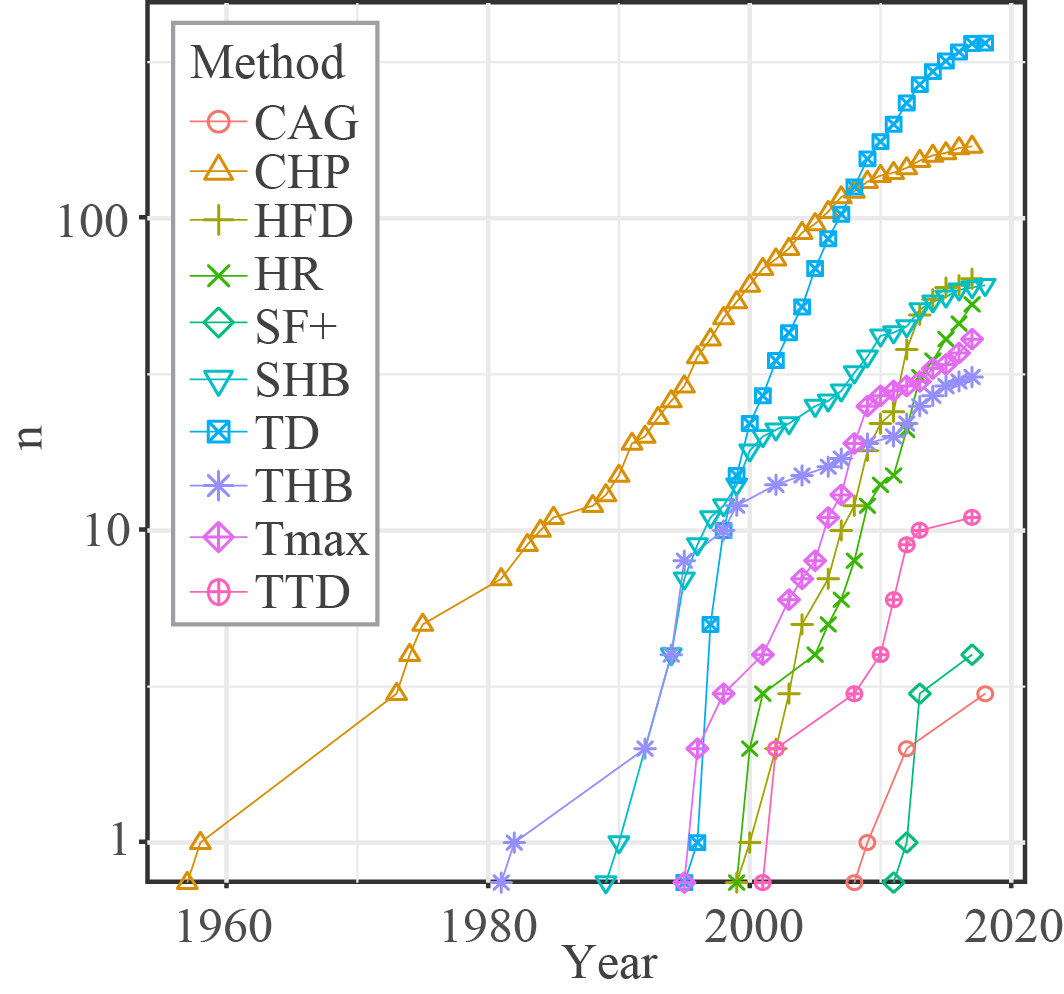
\includegraphics[width=0.8\linewidth]{figure/appendixA/fig1} 

}

\caption[Representation of the cumulative number of studies using different sap flow methods between 1957 and 2017]{Representation of the cumulative number of studies using different sap flow methods between 1957 and 2017 (adapted and updated from Poyatos et al. 2016). CAG: calibrated average gradient; CHP: compensation heat pulse (early heat pulse methods have been considered CHP, Edwards et al. 1997); HFD: head field deformation; HR: heat ratio, SF+: sapflow+; SHB: stem heat balance; TD: thermal dissipation; THB: trunk heat balance; Tmax: T-max heat pulse; TTD: transient thermal dissipation. Notice the logarithmic scale on the y-axis.}\label{fig:apa11}
\end{figure}
\setlength{\abovecaptionskip}{0pt} \newpage

\setlength{\abovecaptionskip}{15pt}
\begin{figure}[hbt!]

{\centering 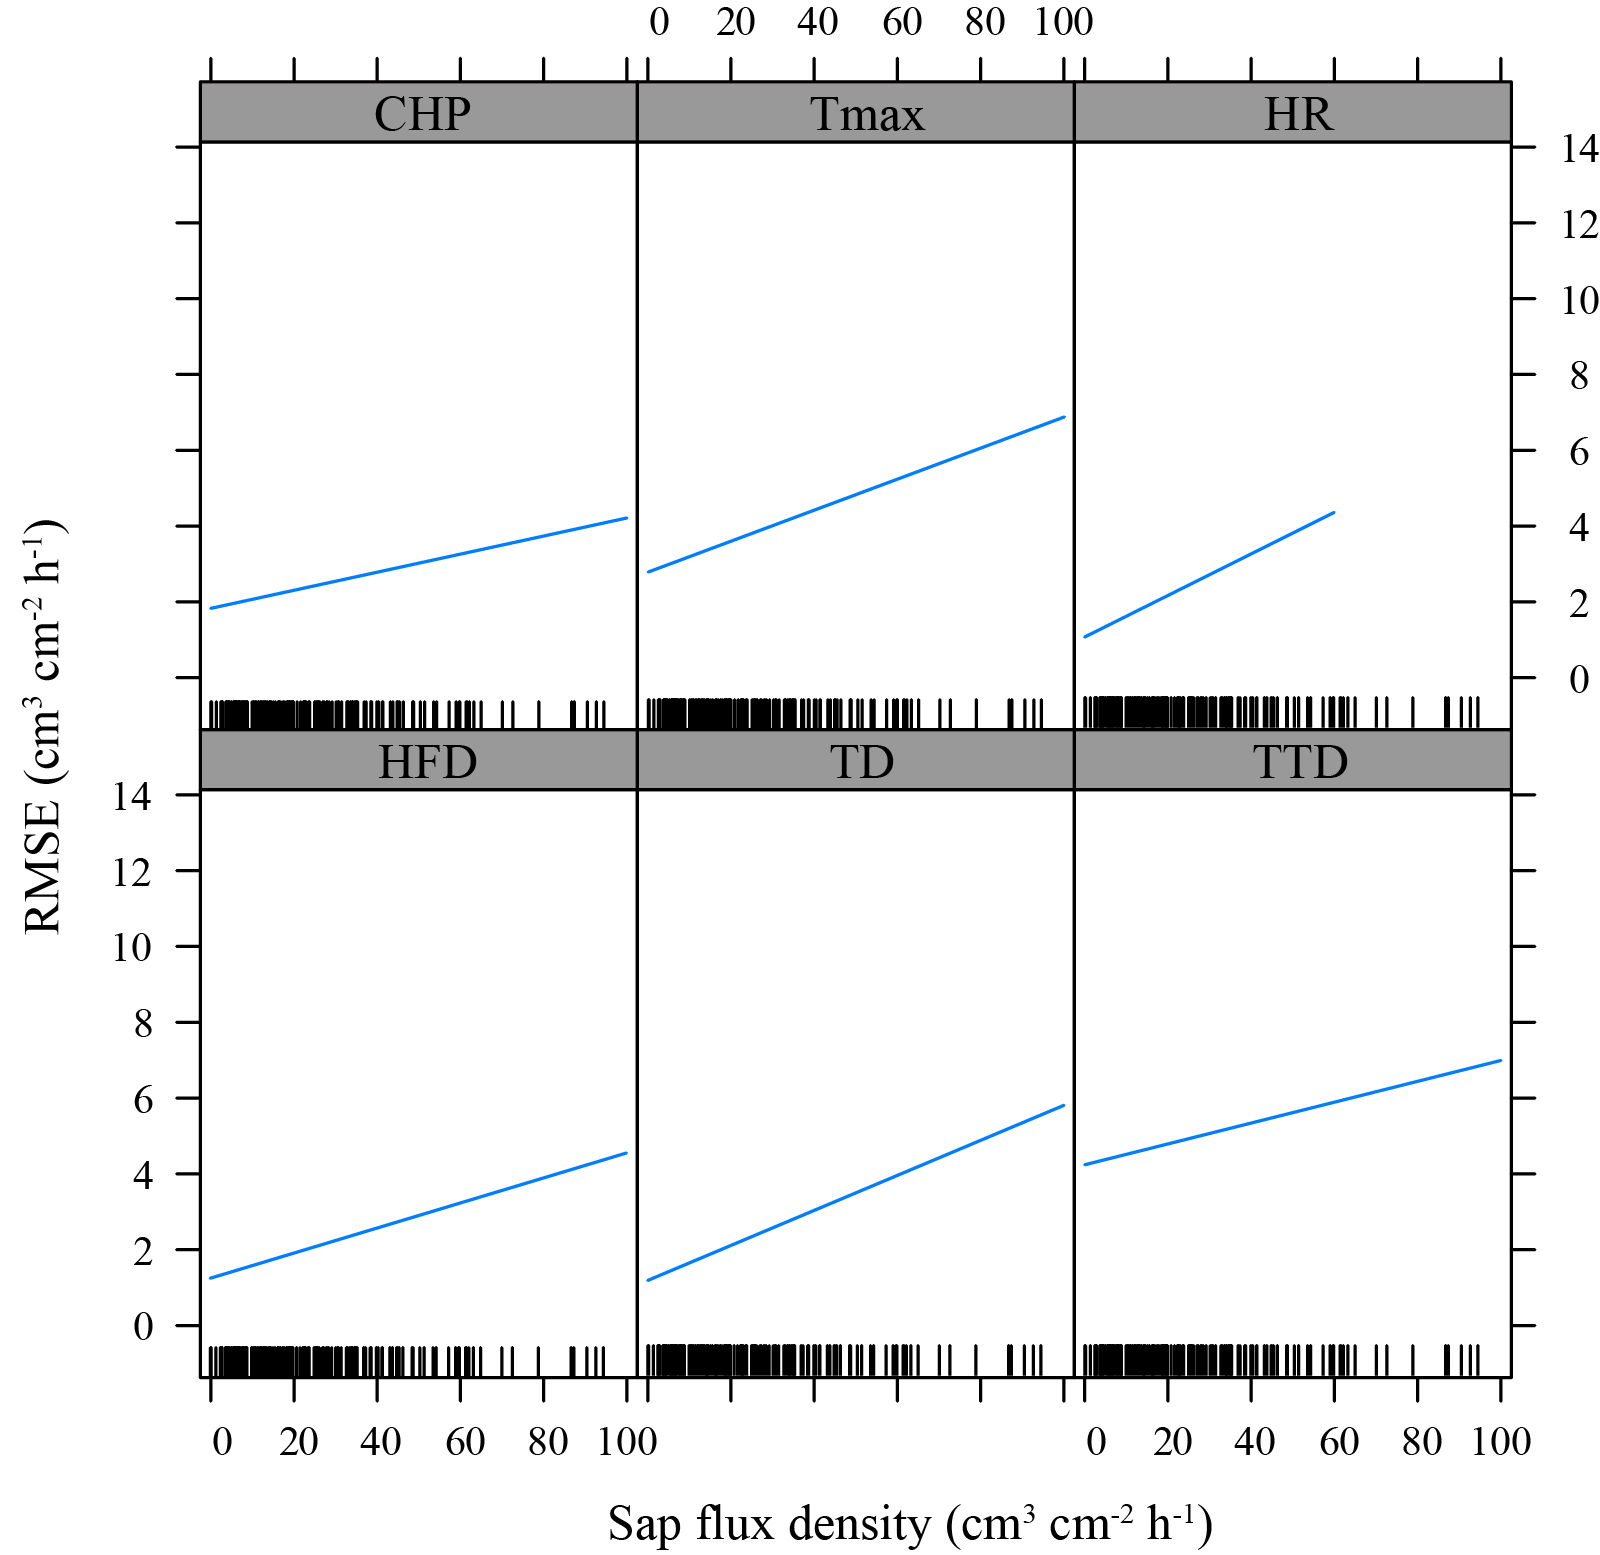
\includegraphics[width=1\linewidth]{figure/appendixA/fig2} 

}

\caption[Relationship between root mean square error (RMSE) and sap flux density.]{Relationship between root mean square error (RMSE) and sap flux density (mean calibration range) and for different sap flux density methods, as predicted by the LMM model presented in Table 3.}\label{fig:apa122}
\end{figure}
\setlength{\abovecaptionskip}{0pt}

\newpage
\begin{figure}[hbt!]

{\centering 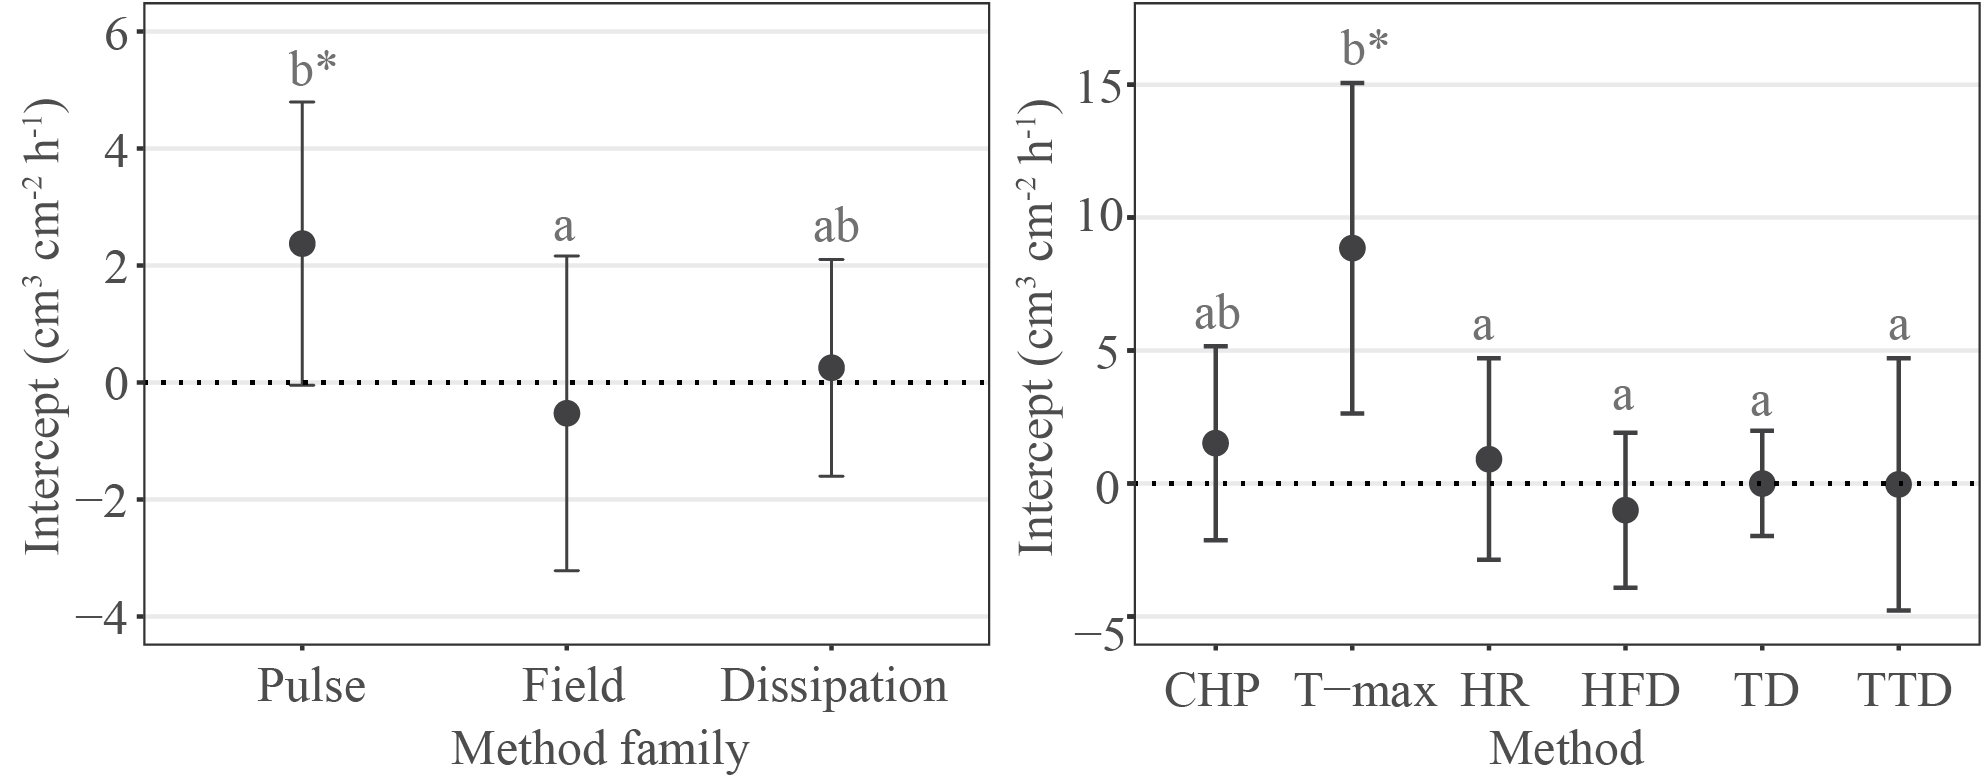
\includegraphics[width=1\linewidth]{figure/appendixA/fig3} 

}

\caption[Predictions of the LMM models calculated from least-squares means of the intercept ($\beta_{0}$) of the linear model.]{Predictions of the LMM models calculated from least-squares means of the intercept ($\beta_{0}$) of the linear model (Eq. 3). Different letters indicate significant differences between factors levels evaluated with Tukey’s test. Horizontal, dotted lines indicate reference, perfect calibration values for a given metric. Asterisks (*) indicate significant (p<0.05) departure from those reference values.}\label{fig:apa13}
\end{figure}\newpage
\section{Tables A}\label{tables-a}

\begingroup\fontsize{6}{8}\selectfont
\begin{longtable}[t]{>{\raggedright\arraybackslash}p{12em}>{\raggedright\arraybackslash}p{3em}l>{\raggedright\arraybackslash}p{6em}l>{\raggedleft\arraybackslash}p{3em}}
\caption[Summary table of the studies used in the analyses.]{\label{tab:unnamed-chunk-1}Summary table of the studies used in the analyses presented in the paper. Sap flow method, species, calibration material, porosity and average stem/tree diameter are reported.}\\
\toprule
Study & Method & Species & Calibration material & Wood porosity & Diameter (cm)\\
\midrule
\endfirsthead
\caption[]{\label{tab:unnamed-chunk-1}Summary table of the studies used in the analyses presented in the paper. Sap flow method, species, calibration material, porosity and average stem/tree diameter are reported. \textit{(continued)}}\\
\toprule
Study & Method & Species & Calibration material & Wood porosity & Diameter (cm)\\
\midrule
\endhead
\
\endfoot
\bottomrule
\endlastfoot
Alarcon $et\;\, al.$ 2005 & CHP & $Citrus\;\,limon$ & whole plant & Diffuse porous & 2.50\\
Ballester et al 2011 & CHP & $Citrus\;\,clementina$ & whole plant & Diffuse porous & NA\\
Barret $et\;\, al.$ 1995 & CHP & $Corymbia\;\,maculata$ & without roots & Diffuse porous & NA\\
Bleby $et\;\, al.$ 2004 & CHP & $Eucalyptus\;\,marginata$ & whole plant & Diffuse porous & 10.00\\
Bleby $et\;\, al.$ 2004 & HR & $Eucalyptus\;\,marginata$ & whole plant & Diffuse porous & 10.00\\
Braun and Schmid 1999 & TD & $Vitis\;\,vinifera$ & whole plant & Ring porous & 3.75\\
Burgess $et\;\, al.$ 2001 & HR & $Eucalyptus\;\,marginata$ & whole plant & Diffuse porous & NA\\
Bush $et\;\, al.$ 2010 & TD & $Populus\;\,fremontii$ & stem segment & Diffuse porous & 5.08\\
Bush $et\;\, al.$ 2010 & TD & $Tilia\;\,cordata$ & stem segment & Diffuse porous & 4.83\\
Cain 2009 & TD & $Macaranga\;\,hypoleuca$ & stem segment & Diffuse porous & 82.00\\
Cain 2009 & TD & $Macaranga\;\,pearsonii$ & stem segment & Diffuse porous & 67.00\\
Caspari $et\;\, al.$ 1993 & CHP & $Pyrus\;\,serotina$ & whole plant & Diffuse porous & 6.62\\
Caterina $et\;\, al.$ 2013 & TD & $Juniperus\;\,virginiana$ & stem segment & Tracheids & 8.00\\
Chan 2015 & TD & $Abies\;\,concolor$ & stem segment & Tracheids & 6.00\\
Cohen $et\;\, al.$ 1981 & T-max & $Platanus\;\,orientalis$ & stem segment & Diffuse porous & 6.70\\
Cohen $et\;\, al.$ 1981 & T-max & $Populus\;\,alba$ & stem segment & Diffuse porous & 6.70\\
Cohen $et\;\, al.$ 1998 & T-max & $Malus\;\,domestica$ & whole plant & Diffuse porous & NA\\
Dragoni $et\;\, al.$ 2005 & CHP & $Malus\;\,domestica$ & whole plant & Diffuse porous & 6.50\\
Dye $et\;\, al.$ 1996 & CHP & $Pinus\;\,patula$ & without roots & Tracheids & NA\\
Fernandez $et\;\, al.$ 1999 & CHP & $Olea\;\,europaea$ & stem segment & Diffuse porous & 8.80\\
Fernandez $et\;\, al.$ 1999 & CHP & $Olea\;\,europaea$ & without roots & Diffuse porous & NA\\
Fernandez $et\;\, al.$ 2006 & CHP & $Citrus\;\,sinensis$ & stem segment & Diffuse porous & 7.80\\
Fernandez $et\;\, al.$ 2006 & CHP & $Citrus\;\,sinensis$ & without roots & Diffuse porous & 10.40\\
Fernandez $et\;\, al.$ 2006 & CHP & $Olea\;\,europaea$ & stem segment & Diffuse porous & 8.20\\
Fernandez $et\;\, al.$ 2006 & CHP & $Olea\;\,europaea$ & without roots & Diffuse porous & 9.80\\
Fernandez $et\;\, al.$ 2006 & CHP & $Prunus\;\,domestica$ & stem segment & Diffuse porous & 8.00\\
Fernandez $et\;\, al.$ 2006 & CHP & $Prunus\;\,domestica$ & without roots & Diffuse porous & 7.00\\
Fuchs $et\;\, al.$ 2017 & HFD & $Acer\;\,pseudoplatanus$ & stem segment & Diffuse porous & 10.56\\
Fuchs $et\;\, al.$ 2017 & HFD & $Fagus\;\,sylvatica$ & stem segment & Diffuse porous & 9.42\\
Fuchs $et\;\, al.$ 2017 & HFD & $Tilia\;\,cordata$ & stem segment & Diffuse porous & 9.29\\
Fuchs $et\;\, al.$ 2017 & HR & $Acer\;\,pseudoplatanus$ & stem segment & Diffuse porous & NA\\
Fuchs $et\;\, al.$ 2017 & HR & $Fagus\;\,sylvatica$ & stem segment & Diffuse porous & NA\\
Fuchs $et\;\, al.$ 2017 & HR & $Tilia\;\,cordata$ & stem segment & Diffuse porous & NA\\
Fuchs $et\;\, al.$ 2017 & TD & $Acer\;\,campestre$ & stem segment & Diffuse porous & 11.81\\
Fuchs $et\;\, al.$ 2017 & TD & $Acer\;\,pseudoplatanus$ & stem segment & Diffuse porous & 10.80\\
Fuchs $et\;\, al.$ 2017 & TD & $Fagus\;\,sylvatica$ & stem segment & Diffuse porous & 9.83\\
Fuchs $et\;\, al.$ 2017 & TD & $Populus\;\,nigra$ & stem segment & Diffuse porous & 10.77\\
Fuchs $et\;\, al.$ 2017 & TD & $Tilia\;\,cordata$ & stem segment & Diffuse porous & 9.41\\
Gonzalez-Altozano $et\;\, al.$ 1998 & CHP & $Citrus\;\,reticulata$ & whole plant & Diffuse porous & 11.50\\
Gonzalez-Altozano $et\;\, al.$ 1998 & T-max & $Citrus\;\,reticulata$ & whole plant & Diffuse porous & 11.50\\
Granier 1985 & TD & $Pinus\;\,nigra$ & stem segment & Tracheids & 4.50\\
Granier 1985 & TD & $Pseudotzuga\;\,menziesii$ & stem segment & Tracheids & 4.50\\
Granier 1985 & TD & $Quercus\;\,pedunculata$ & stem segment & Ring porous & 4.50\\
Green $et\;\, al.$ 1988 & CHP & $Actinidia\;\,chinensis$ & stem segment & Diffuse porous & 5.25\\
Green $et\;\, al.$ 1988 & CHP & $Actinidia\;\,chinensis$ & whole plant & Diffuse porous & 5.40\\
Green $et\;\, al.$ 1988 & CHP & $Malus\;\,sylvestris$ & whole plant & Diffuse porous & 5.60\\
Gutierrez $et\;\, al.$ 1994 & SHB & $Acacia\;\,koa$ & whole plant & Diffuse porous & NA\\
Gutierrez $et\;\, al.$ 1994 & SHB & $Coffea\;\,arabica$ & whole plant & Diffuse porous & NA\\
Gutierrez Soto $et\;\, al.$ 2012 & HR & $Carica\;\,papaya$ & whole plant & Monocot & NA\\
Hatton $et\;\, al.$ 1995 & CHP & $Eucalyptus\;\,populnea$ & without roots & Diffuse porous & 5.40\\
Heilman $et\;\, al.$ 1990 & SHB & $Ligustrum\;\,japonicum$ & whole plant & Diffuse porous & 1.00\\
Herbs $et\;\, al.$ 2007 & TD & $Acer\;\,campestre$ & stem segment & Diffuse porous & NA\\
Herbs $et\;\, al.$ 2007 & TD & $Crataegus\;\,monogina$ & stem segment & Diffuse porous & NA\\
Hultine $et\;\, al.$ 2010 & TD & $Tamarix\;\,ramossisima$ & stem segment & Ring porous & 4.16\\
Intrigliolo $et\;\, al.$ 2009 & T-max & $Vitis\;\,vinifera$ & whole plant & Ring porous & NA\\
Isarangkool $et\;\, al.$ 2009 & TTD & $Abies\;\,concolor$ & stem segment & Diffuse porous & 5.14\\
Isarangkool $et\;\, al.$ 2009 & TTD & $Hevea\;\,brasiliensis$ & stem segment & Diffuse porous & 4.69\\
Isarangkool $et\;\, al.$ 2009 & TTD & $Mangifera\;\,indica$ & stem segment & Diffuse porous & 4.35\\
Johan Uddling $et\;\, al.$ 2009 & TD & $Betula\;\,papyrifera$ & stem segment & Diffuse porous & NA\\
Lu 2002 & TD & $Garcinia\;\,mangostana$ & whole plant & Diffuse porous & 4.00\\
Lu 2002 & TD & $Mangifera\;\,indica$ & whole plant & Diffuse porous & 2.30\\
Lu 2002 & TD & $Musa\;\,spp.$ & whole plant & Monocot & 12.00\\
Lu and Chacko 1998 & TD & $Mangifera\;\,indica$ & whole plant & Diffuse porous & 2.30\\
Madurapperuma $et\;\, al.$ 2009 & HR & $Syagrus\;\,romanzoffiana$ & whole plant & Monocot & NA\\
Michell $et\;\, al.$ 2009 & HR & $Eucalyptus\;\,capillosa$ & without roots & Diffuse porous & 6.50\\
Montague $et\;\, al.$ 2006 & TD & $Liquidambar\;\,styraciflua$ & whole plant & Diffuse porous & 5.30\\
Montague $et\;\, al.$ 2006 & TD & $Populus\;\,deltoides$ & whole plant & Diffuse porous & 5.60\\
Montague $et\;\, al.$ 2006 & TD & $Pyrus\;\,calleryana$ & whole plant & Diffuse porous & 6.60\\
Montague $et\;\, al.$ 2006 & TD & $Quercus\;\,robur\;\,x\;\,Q.\;\,Bicolor$ & whole plant & Ring porous & 5.70\\
Nadezhdina $et\;\, al.$ 1998 & HFD & $Tilia\;\,cordata$ & without roots & Diffuse porous & 12.00\\
Nortes $et\;\, al.$ 2009 & CHP & $Prunus\;\,dulcis$ & whole plant & Diffuse porous & 15.00\\
Paudel $et\;\, al.$ 2013 & TD & $Malus\;\,domestica$ & stem segment & Diffuse porous & 4.01\\
Paudel $et\;\, al.$ 2013 & TD & $Peltophorum\;\,dubium$ & stem segment & Diffuse porous & 3.70\\
Paudel $et\;\, al.$ 2013 & TD & $Prunus\;\,persica$ & stem segment & Diffuse porous & 4.00\\
Paudel $et\;\, al.$ 2013 & TTD & $Malus\;\,domestica$ & stem segment & Diffuse porous & 4.01\\
Paudel $et\;\, al.$ 2013 & TTD & $Peltophorum\;\,dubium$ & stem segment & Diffuse porous & 3.70\\
Paudel $et\;\, al.$ 2013 & TTD & $Prunus\;\,persica$ & stem segment & Diffuse porous & 4.00\\
Peters $et\;\, al.$ 2017 & TD & $Larix\;\,decidua$ & stem segment & Tracheids & 16.50\\
Peters $et\;\, al.$ 2017 & TD & $Picea\;\,abies$ & stem segment & Tracheids & 15.90\\
Prendergast $et\;\, al.$ 2007 & T-max & $Actinidia\;\,chinensis$ & stem segment & Diffuse porous & 9.50\\
Shackel $et\;\, al.$ 1992 & SHB & $Prunus\;\,persica$ & whole plant & Diffuse porous & 6.25\\
Smith $et\;\, al.$ 1995 & CHP & $Acacia\;\,holosericea$ & stem segment & Diffuse porous & NA\\
Smith $et\;\, al.$ 1995 & CHP & $Acacia\;\,holosericea$ & without roots & Diffuse porous & NA\\
Smith $et\;\, al.$ 1995 & CHP & $Acacia\;\,nilotica$ & stem segment & Diffuse porous & NA\\
Smith $et\;\, al.$ 1995 & CHP & $Azadirachta\;\,indica$ & stem segment & Diffuse porous & NA\\
Smith $et\;\, al.$ 1995 & CHP & $Azadirachta\;\,indica$ & without roots & Diffuse porous & NA\\
Sperling $et\;\, al.$ 2012 & TD & $Phoenix\;\,datylifera$ & whole plant & Monocot & 60.00\\
Steppe $et\;\, al.$ 2010 & CHP & $Fagus\;\,grandifolia$ & stem segment & Diffuse porous & 18.00\\
Steppe $et\;\, al.$ 2010 & HFD & $Fagus\;\,grandifolia$ & stem segment & Diffuse porous & 18.12\\
Steppe $et\;\, al.$ 2010 & TD & $Fagus\;\,grandifolia$ & stem segment & Diffuse porous & 18.00\\
Sun $et\;\, al.$ 2012 & TD & $Liquidambar\;\,styraciflua$ & without roots & Diffuse porous & 7.50\\
Sun $et\;\, al.$ 2012 & TD & $Pinus\;\,echinata$ & without roots & Tracheids & 7.50\\
Sun $et\;\, al.$ 2012 & TD & $Pinus\;\,taeda$ & without roots & Tracheids & 7.50\\
Sun $et\;\, al.$ 2012 & TD & $Populus\;\,deltoides$ & without roots & Diffuse porous & 7.50\\
Sun $et\;\, al.$ 2012 & TD & $Quercus\;\,alba$ & without roots & Ring porous & 7.50\\
Sun $et\;\, al.$ 2012 & TD & $Ulmus\;\,americana$ & without roots & Ring porous & 7.50\\
Swanson and Whitfield 1981 & CHP & $Nothofagus\;\,solandri$ & whole plant & Diffuse porous & 11.00\\
Swanson and Whitfield 1981 & CHP & $Pinus\;\,radiata$ & whole plant & Tracheids & 5.00\\
Urban $et\;\, al.$ 2012 & SHB & $Humulus\;\,lupulus$ & without roots & Ring porous & NA\\
Vellame $et\;\, al.$ 2010 & SHB & $Citrus\;\,sinensis$ & whole plant & Diffuse porous & 1.40\\*
\end{longtable}
\endgroup{}

\newpage
\begin{table}[!h]

\caption[Anova summary of the LMM models.]{\label{tab:unnamed-chunk-2}Anova summary of the LMM models, using the same structure as objective 1, comparing calibrations reported in SFD and SF units (Units) for CHP and TD. CM (Calibration material).}
\centering
\fontsize{6}{8}\selectfont
\begin{tabular}[t]{ccccccccc}
\toprule
Method & Calibration metric & Variable & Sum sq & Mean Sq & NumDF & DenDF & F.value & Pr(>F)\\
\midrule
 &  & Units & 0.09 & 0.09 & 1 & 52.05 & 1.09 & 0.302\\
\cmidrule{3-9}
 & \multirow[t]{-2}{*}{\centering\arraybackslash Ln-Ratio} & CM & 0.20 & 0.10 & 2 & 44.43 & 1.24 & 0.299\\
\cmidrule{2-9}
 &  & Units & 0.07 & 0.07 & 1 & 25.27 & 0.37 & 0.55\\
\cmidrule{3-9}
 & \multirow[t]{-2}{*}{\centering\arraybackslash Slope} & CM & 0.24 & 0.12 & 2 & 40.07 & 0.59 & 0.558\\
\cmidrule{2-9}
 &  & Units & 0.00 & 0.00 & 1 & 12.35 & 0.02 & 0.89\\
\cmidrule{3-9}
 & \multirow[t]{-2}{*}{\centering\arraybackslash Slope (ln-ln)} & CM & 0.14 & 0.07 & 2 & 22.13 & 0.91 & 0.416\\
\cmidrule{2-9}
 &  & Units & 1.07 & 1.07 & 1 & 20.77 & 4.30 & 0.051 .\\
\cmidrule{3-9}
\multirow[t]{-8}{*}{\centering\arraybackslash CHP} & \multirow[t]{-2}{*}{\centering\arraybackslash Z-Cor} & CM & 4.63 & 2.32 & 2 & 34.98 & 9.28 & 0.001 ***\\
\cmidrule{1-9}
 &  & Units & 0.05 & 0.05 & 1 & 26.72 & 0.41 & 0.529\\
\cmidrule{3-9}
 & \multirow[t]{-2}{*}{\centering\arraybackslash Ln-Ratio} & CM & 0.14 & 0.07 & 2 & 16.64 & 0.58 & 0.571\\
\cmidrule{2-9}
 &  & Units & 0.16 & 0.16 & 1 & 44.72 & 2.28 & 0.138\\
\cmidrule{3-9}
 & \multirow[t]{-2}{*}{\centering\arraybackslash Slope} & CM & 0.17 & 0.08 & 2 & 14.84 & 1.17 & 0.338\\
\cmidrule{2-9}
 &  & Units & 0.22 & 0.22 & 1 & 72.67 & 2.18 & 0.144\\
\cmidrule{3-9}
 & \multirow[t]{-2}{*}{\centering\arraybackslash Slope (ln-ln)} & CM & 0.14 & 0.07 & 2 & 29.27 & 0.71 & 0.501\\
\cmidrule{2-9}
 &  & Units & 0.08 & 0.08 & 1 & 26.07 & 0.28 & 0.598\\
\cmidrule{3-9}
\multirow[t]{-8}{*}{\centering\arraybackslash TD} & \multirow[t]{-2}{*}{\centering\arraybackslash Z-Cor} & CM & 0.02 & 0.01 & 2 & 17.41 & 0.03 & 0.969\\
\bottomrule
\end{tabular}
\end{table}
\newpage
\begin{landscape}
\begin{table}

\caption[Summary of the LMM models of Ln-Ratio (accuracy), Slope (proportional bias), Slope (ln-ln) (linearity) and Z-Cor (precision) as a function of Methods and Calibration material.]{\label{tab:unnamed-chunk-3}Summary of the LMM models of Ln-Ratio (accuracy), Slope (proportional bias), Slope (ln-ln) (linearity) and Z-Cor (precision) as a function of Methods and Calibration material (CM; Whole plant: whole plant on a container or lysimeter; No-roots: whole plant without roots). CHP is the reference level for the variable Method and Stem segment is the reference level for CM, corresponding to the model intercept. All other coefficient estimates indicate the difference relative to the intercept. $\sigma^{2}$ is the within-groups random variability (residuals of the model). $\tau_{00}$ is the between-group random variability. N is the number of levels within random groups. ICC is the Intraclass Correlation Coefficients of each random group. $R^{2}m$ and $R^{2}c$ are the variability explained by the fixed and the random factors, respectively.}
\centering
\resizebox{\linewidth}{!}{
\fontsize{5}{7}\selectfont
\begin{tabular}[t]{ccccccccccccc}
\toprule
Coefficients & Estimate & Conf. Int. & p-value & Estimate & Conf. Int. & p-value & Estimate & Conf. Int. & p-value & Estimate & Conf. Int. & p-value\\
\midrule
Fixed effects &  &  &  &  &  &  &  &  &  &  &  & \\
(Intercept) & 0.19 & -0.052\: , \:0.425 & 0.129 & 0.96 & 0.779\: , \:1.135 & <0.001 & 0.85 & 0.719\: , \:0.976 & <0.001 & 2.32 & 1.982\: , \:2.653 & 2.32\\
Method (T-max) & -0.19 & -0.611\: , \:0.240 & 0.395 & -0.27 & -0.584\: , \:0.038 & 0.089 & -0.08 & -0.312\: , \:0.142 & 0.463 & -0.08 & -0.669\: , \:0.506 & -0.08\\
Method (HR) & -0.28 & -0.510\: , \:-0.047 & 0.019 & -0.04 & -0.247\: , \:0.162 & 0.683 & 0.06 & -0.106\: , \:0.221 & 0.488 & 0.16 & -0.205\: , \:0.525 & 0.16\\
Method (HFD) & -0.21 & -0.409\: , \:-0.003 & 0.048 & 0.01 & -0.167\: , \:0.193 & 0.886 & 0.00 & -0.143\: , \:0.143 & 1 & 0.54 & 0.220\: , \:0.862 & 0.54\\
Method (SHB) & -0.37 & -0.843\: , \:0.095 & 0.124 & -0.04 & -0.365\: , \:0.285 & 0.809 & 0.18 & -0.058\: , \:0.427 & 0.139 & 0.45 & -0.170\: , \:1.070 & 0.45\\
Method (TD) & -0.65 & -0.847\: , \:-0.457 & <0.001 & -0.20 & -0.368\: , \:-0.041 & 0.015 & 0.28 & 0.160\: , \:0.406 & <0.001 & -0.12 & -0.423\: , \:0.173 & -0.12\\
Method (TTD) & -0.62 & -0.941\: , \:-0.310 & <0.001 & -0.22 & -0.503\: , \:0.066 & 0.134 & 0.20 & -0.016\: , \:0.421 & 0.072 & -0.37 & -0.877\: , \:0.133 & -0.37\\
CM (Whole plant) & -0.03 & -0.300\: , \:0.245 & 0.841 & -0.13 & -0.317\: , \:0.064 & 0.197 & -0.14 & -0.276\: , \:-0.003 & 0.05 & -0.67 & -1.034\: , \:-0.301 & -0.67\\
CM (No-roots) & -0.13 & -0.394\: , \:0.128 & 0.319 & -0.08 & -0.298\: , \:0.135 & 0.463 & -0.06 & -0.213\: , \:0.104 & 0.503 & -0.78 & -1.172\: , \:-0.379 & -0.78\\
Random effects &  &  &  &  &  &  &  &  &  &  &  & \\
$\sigma^{2}$ &  & 0.091 &  &  & 0.1 &  &  & 0.076 &  &  & 0.278 & \\
$\tau_{00}$ Species &  & 0.013 &  &  & 0.004 &  &  & 0.013 &  &  & 0.04 & \\
$\tau_{00}$ Study &  & 0.159 &  &  & 0.041 &  &  & 0.004 &  &  & 0.184 & \\
$N_{Species}$ &  & 65 &  &  & 65 &  &  & 65 &  &  & 65 & \\
$N_{Study}$ &  & 48 &  &  & 48 &  &  & 48 &  &  & 48 & \\
$ICC_{Species}$ &  & 0.049 &  &  & 0.029 &  &  & 0.137 &  &  & 0.08 & \\
$ICC_{Study}$ &  & 0.604 &  &  & 0.284 &  &  & 0.048 &  &  & 0.366 & \\
Observations &  & 290 &  &  & 290 &  &  & 290 &  &  & 290 & \\
\bottomrule
\end{tabular}}
\end{table}
\end{landscape}
\newpage

\chapter{Appendix Chapter 4}\label{appendix-chapter-4}

\newpage

\section{Figures C}\label{figures-c}

\setlength{\abovecaptionskip}{15pt}
\begin{figure}[H]

{\centering 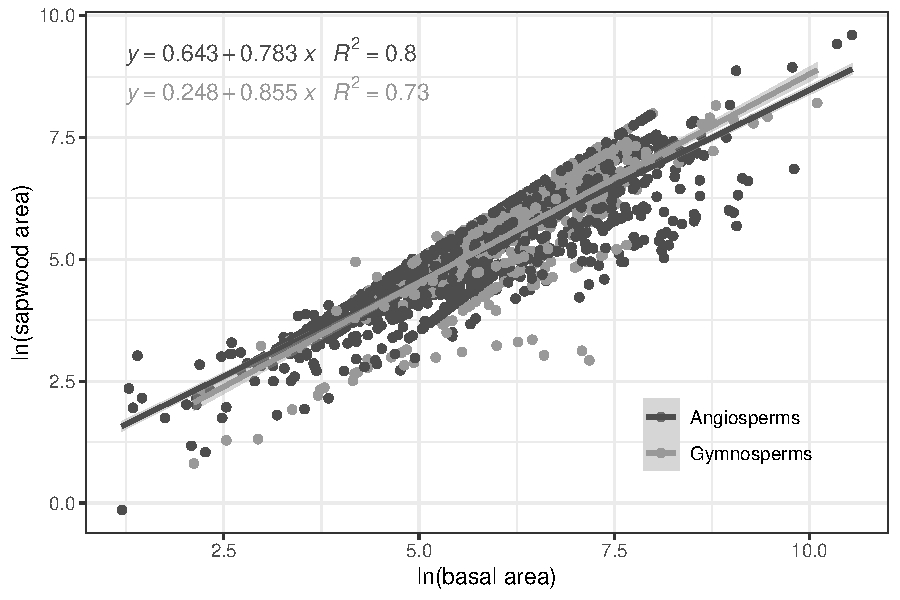
\includegraphics[width=1\linewidth]{figure/appendixC/dbh_sw} 

}

\caption[SAPFLUXNET global scaling relationship between basal area and sapwood area. Shaded areas are 95\% model confidence interval.]{SAPFLUXNET global scaling relationship between basal area and sapwood area. Shaded areas are 95\% model confidence interval.}\label{fig:unnamed-chunk-4}
\end{figure}
\setlength{\abovecaptionskip}{0pt}

\newpage

\setlength{\abovecaptionskip}{15pt}
\begin{figure}[H]

{\centering 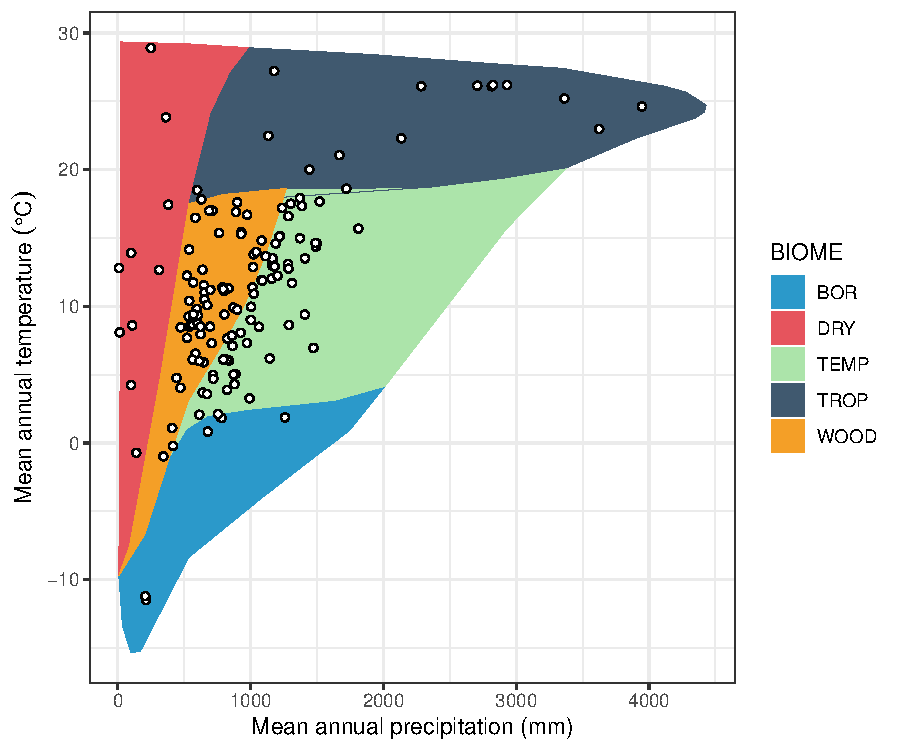
\includegraphics[width=1\linewidth]{figure/appendixC/gg_biomes} 

}

\caption[Bioclimatic distribution of the SAPFLUXNET datasets used in the study.]{Bioclimatic distribution of the SAPFLUXNET datasets used in the study. Points show the different datasets in a Whittaker diagram showing the classification of the aggregated biomes used in the study.}\label{fig:unnamed-chunk-5}
\end{figure}
\setlength{\abovecaptionskip}{0pt}

\newpage

\setlength{\abovecaptionskip}{15pt}
\begin{figure}[H]

{\centering \includegraphics[width=1\linewidth]{figure/appendixC/var_maps} 

}

\caption[Global projection of climatic, soil and stand structure variables.]{Global projection of climatic, soil and stand structure variables. log(PPET): logarithm of precipitation over potential evapotraspiration [log(mm \text{$mm^{-1}$})]; log(\text{$P-PET_{sd}$}): logarithm of the standard deviation of the difference between precipitation and potential evapotranspiration [log(mm)]; Clay: percentage of clay in the soil; Total N: total nitrogen in the soil [g \text{$kg^{-1}$}];  Bedrock [cm]; Stand height [m]; LAI: leaf area index [\text{$m^2$ $m^{-2}$}]. Total N values above 5 g \text{$kg^{-1}$} were truncated.}\label{fig:unnamed-chunk-6}
\end{figure}
\setlength{\abovecaptionskip}{0pt}

\newpage

\setlength{\abovecaptionskip}{15pt}
\begin{figure}[hbt!]

{\centering 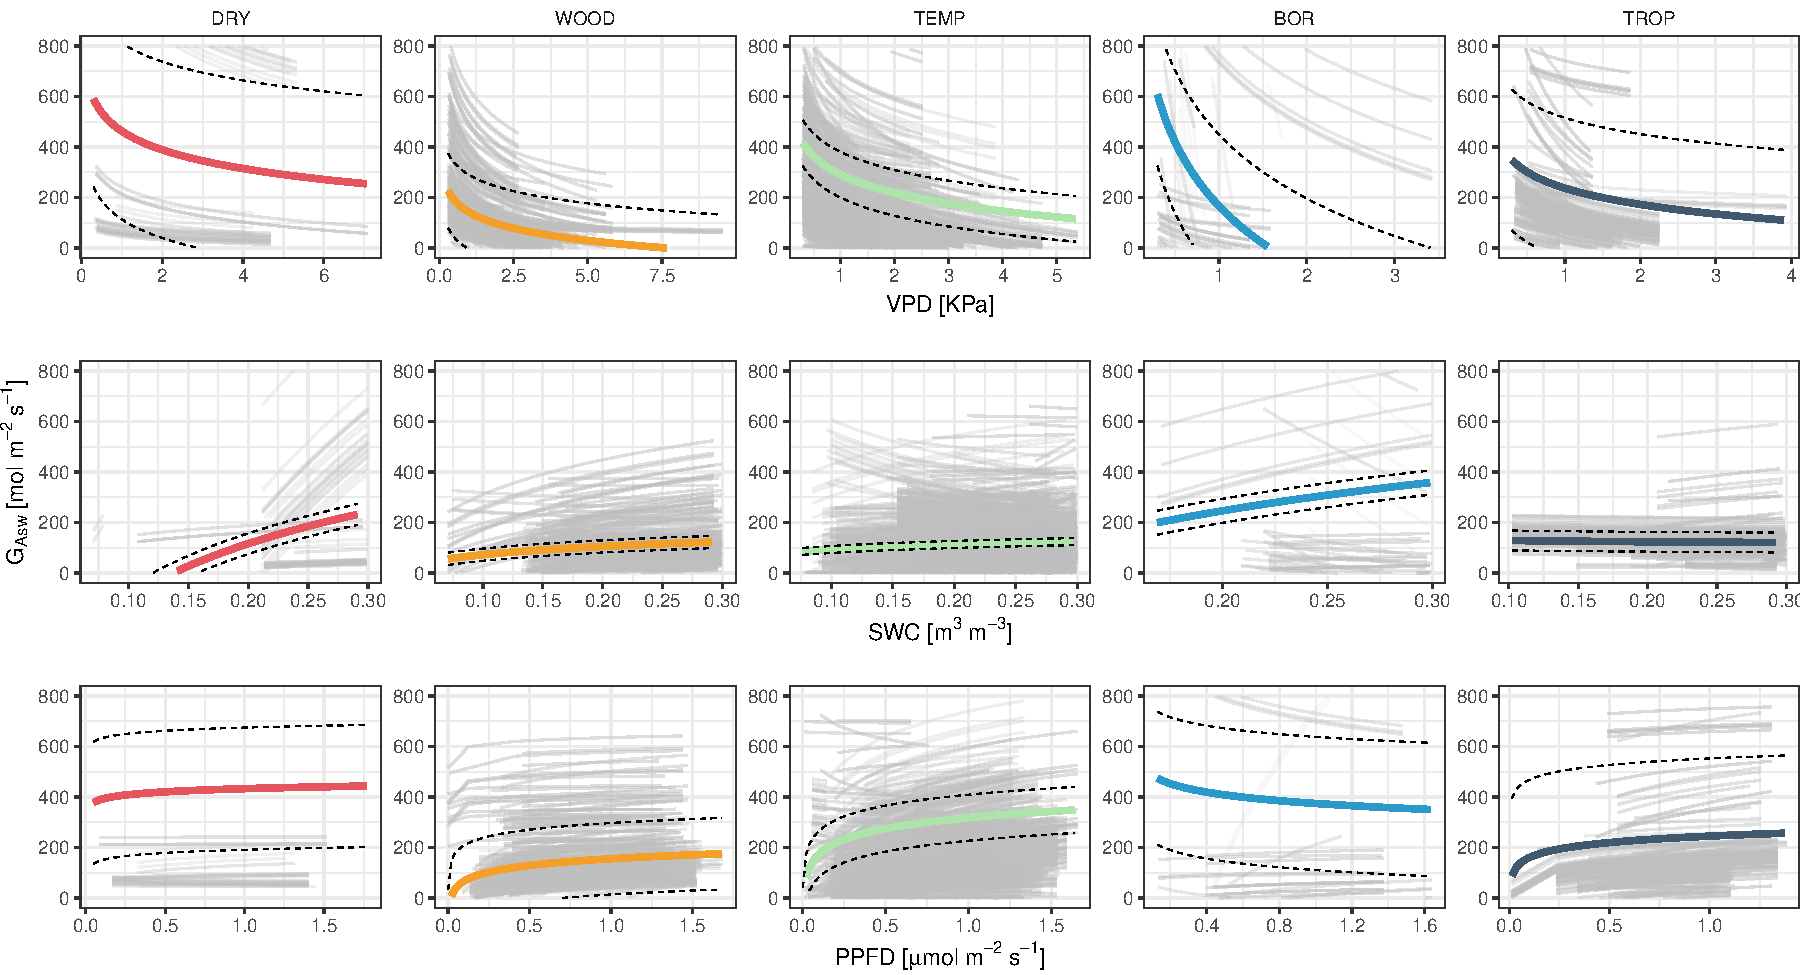
\includegraphics[width=1\linewidth]{figure/appendixC/spa_plots} 

}

\caption[Log relationships of the three environmental variables estimated with the TOTAL model (VPD + SWC + PPFD) and grouped by biome.]{Log relationships of the three environmental variables estimated with the TOTAL model (VPD + SWC + PPFD) and grouped by biome. Coloured lines are biome average models calculated from the Log-linear models predictions using LMM with Gs as response variable and the neperian logarithm of the environmental constrains as explanatory variables. Dashed line shows standard error of the average models calculated with bootstrap prediction using 100 simulations.}\label{fig:unnamed-chunk-7}
\end{figure}
\setlength{\abovecaptionskip}{0pt} \newpage

\section{Tables C}\label{tables-c}

\begingroup\fontsize{6}{8}\selectfont
\begin{longtable}[t]{ccccccc}
\caption[SAPFLUXNET sites included in the study. Biome was calculated using Whittaker diagram.]{\label{tab:unnamed-chunk-8}SAPFLUXNET sites included in the study. Biome was calculated using Whittaker diagram. *Indicates that the biome was manually adjusted and confirmed by SAPFLUXNET contributors.}\\
\toprule
Site code & Latitude & Longitude & Biome & \# Tree-days & \# Species & \# Trees\\
\midrule
\endfirsthead
\caption[]{\label{tab:unnamed-chunk-8}SAPFLUXNET sites included in the study. Biome was calculated using Whittaker diagram. *Indicates that the biome was manually adjusted and confirmed by SAPFLUXNET contributors. \textit{(continued)}}\\
\toprule
Site code & Latitude & Longitude & Biome & \# Tree-days & \# Species & \# Trees\\
\midrule
\endhead
\
\endfoot
\bottomrule
\endlastfoot
AUS\_CAN\_ST1\_EUC & -37.58 & 149.17 & WOOD & 337 & 1 & 12\\
AUS\_CAN\_ST2\_MIX & -37.58 & 149.17 & WOOD & 712 & 2 & 22\\
AUS\_CAN\_ST3\_ACA & -37.58 & 149.17 & WOOD & 409 & 1 & 12\\
AUS\_CAR\_THI\_CON & -38.38 & 146.68 & TEMP & 54 & 1 & 7\\
AUS\_ELL\_UNB & -36.78 & 146.58 & TEMP & 105 & 1 & 2\\
AUS\_MAR\_UBD & -37.69 & 145.56 & TEMP & 50 & 3 & 5\\
AUS\_MAR\_UBW & -37.89 & 145.57 & TEMP & 105 & 3 & 5\\
AUS\_WOM & -37.42 & 144.09 & TEMP & 2130 & 2 & 11\\
AUT\_PAT\_FOR & 47.21 & 11.45 & BOR & 149 & 1 & 3\\
AUT\_PAT\_KRU & 47.21 & 11.45 & BOR & 70 & 1 & 3\\
AUT\_PAT\_TRE & 47.21 & 11.45 & BOR & 81 & 1 & 3\\
BRA\_CAM & -22.69 & -45.52 & TROP & 79 & 1 & 5\\
BRA\_CAX\_CON & -1.79 & -51.43 & TROP & 525 & 8 & 15\\
CAN\_TUR\_P39\_PRE & 42.71 & -80.36 & TEMP & 1021 & 1 & 18\\
CAN\_TUR\_P74 & 42.71 & -80.35 & TEMP & 1997 & 1 & 16\\
CHN\_ARG\_GWS & 41.38 & 89.94 & DRY & 174 & 1 & 2\\
CHN\_HOR\_AFF & 42.72 & 122.37 & WOOD & 1366 & 1 & 16\\
CHN\_YIN\_ST1 & 42.45 & 85.72 & DRY & 105 & 1 & 5\\
CRI\_TAM\_TOW & 10.39 & -84.63 & TROP & 666 & 17 & 26\\
CZE\_BIL\_BIL & 49.25 & 16.69 & TEMP & 238 & 1 & 6\\
CZE\_KRT\_KRT & 49.32 & 16.75 & TEMP & 238 & 1 & 6\\
CZE\_LAN & 48.68 & 16.95 & TEMP & 1093 & 3 & 17\\
CZE\_RAJ\_RAJ & 49.44 & 16.70 & TEMP & 274 & 1 & 6\\
CZE\_SOB\_SOB & 49.25 & 16.69 & TEMP & 655 & 1 & 6\\
CZE\_STI & 49.04 & 17.97 & TEMP & 263 & 1 & 8\\
CZE\_UTE\_BPO & 49.28 & 16.65 & TEMP & 234 & 1 & 6\\
DEU\_HIN\_OAK & 53.33 & 13.19 & TEMP & 482 & 1 & 8\\
DEU\_HIN\_TER & 53.33 & 13.19 & TEMP & 1052 & 2 & 16\\
DEU\_MER\_BEE\_NON & 49.27 & 7.81 & TEMP & 495 & 1 & 8\\
DEU\_MER\_DOU\_NON & 49.27 & 7.81 & TEMP & 491 & 1 & 7\\
DEU\_MER\_MIX\_NON & 49.27 & 7.81 & TEMP & 1108 & 2 & 17\\
DEU\_STE\_2P3 & 53.10 & 13.00 & TEMP & 722 & 1 & 10\\
DEU\_STE\_4P5 & 53.10 & 13.00 & TEMP & 327 & 1 & 10\\
ESP\_ALT\_ARM & 40.78 & -2.33 & WOOD & 1990 & 3 & 15\\
ESP\_ALT\_HUE & 40.79 & -2.29 & WOOD & 967 & 2 & 8\\
ESP\_ALT\_TRI & 40.80 & -2.23 & WOOD & 1522 & 2 & 12\\
ESP\_CAN & 41.43 & 2.07 & WOOD & 2317 & 4 & 21\\
ESP\_GUA\_VAL & 40.90 & -4.03 & WOOD & 2100 & 1 & 24\\
ESP\_LAS & 28.31 & -16.57 & WOOD & 1778 & 1 & 10\\
ESP\_MAJ\_MAI & 39.94 & -5.77 & WOOD & 978 & 1 & 6\\
ESP\_MON\_SIE\_NAT & 41.12 & -3.50 & WOOD & 1250 & 3 & 20\\
ESP\_RIN & 40.60 & -6.02 & WOOD & 502 & 1 & 8\\
ESP\_RON\_PIL & 36.69 & -5.02 & TEMP & 911 & 2 & 12\\
ESP\_TIL\_MIX & 41.33 & 1.01 & WOOD & 3434 & 2 & 32\\
ESP\_TIL\_OAK & 41.33 & 1.01 & WOOD & 717 & 1 & 10\\
ESP\_TIL\_PIN & 41.33 & 1.01 & WOOD & 589 & 1 & 9\\
ESP\_VAL\_BAR & 42.20 & 1.82 & WOOD & 837 & 1 & 12\\
ESP\_VAL\_SOR & 42.20 & 1.81 & WOOD & 1109 & 1 & 13\\
ESP\_YUN\_C1 & 36.72 & -4.97 & WOOD & 619 & 1 & 6\\
ESP\_YUN\_C2 & 36.72 & -4.97 & WOOD & 288 & 1 & 6\\
FIN\_HYY\_SME & 61.85 & 24.29 & TEMP & 34 & 2 & 4\\
FIN\_PET & 69.49 & 27.23 & BOR & 118 & 1 & 7\\
FRA\_FON & 48.48 & 2.78 & TEMP & 276 & 1 & 3\\
FRA\_HES\_HE1\_NON & 48.67 & 7.06 & TEMP & 620 & 1 & 10\\
FRA\_HES\_HE2\_NON & 48.67 & 7.06 & TEMP & 1347 & 1 & 10\\
FRA\_PUE & 43.74 & 3.60 & WOOD & 5229 & 1 & 25\\
GBR\_ABE\_PLO & 56.62 & -3.80 & TEMP & 486 & 1 & 15\\
GBR\_DEV\_CON & 56.03 & -3.72 & TEMP & 133 & 1 & 4\\
GBR\_GUI\_ST1 & 57.27 & -4.82 & TEMP & 398 & 1 & 15\\
GBR\_GUI\_ST2 & 57.27 & -4.82 & TEMP & 298 & 1 & 9\\
GBR\_GUI\_ST3 & 57.27 & -4.82 & TEMP & 249 & 1 & 8\\
GUF\_GUY\_GUY & 5.28 & -52.92 & TROP & 246 & 6 & 6\\
GUF\_GUY\_ST2 & 5.28 & -52.91 & TROP & 369 & 7 & 11\\
GUF\_NOU\_PET & 4.08 & -52.68 & TROP & 562 & 10 & 22\\
HUN\_SIK & 47.93 & 20.44 & WOOD & 365 & 2 & 4\\
ISR\_YAT\_YAT & 31.34 & 35.05 & DRY & 3704 & 1 & 24\\
ITA\_FEI\_S17 & 46.69 & 10.61 & TEMP & 244 & 1 & 6\\
ITA\_KAE\_S20 & 46.70 & 10.61 & BOR & 325 & 1 & 6\\
ITA\_MUN & 46.68 & 10.58 & TEMP & 384 & 1 & 6\\
ITA\_REN & 46.59 & 11.43 & TEMP & 247 & 3 & 8\\
ITA\_RUN\_N20 & 46.70 & 10.64 & BOR & 331 & 2 & 8\\
MEX\_COR\_YP & 19.49 & -97.04 & TEMP & 119 & 1 & 8\\
NLD\_LOO & 52.17 & 5.74 & TEMP & 621 & 1 & 6\\
NLD\_SPE\_DOU & 52.25 & 5.69 & TEMP & 107 & 1 & 3\\
NZL\_HUA\_HUA & -36.80 & 174.49 & TEMP & 243 & 1 & 6\\
PRT\_LEZ\_ARN & 38.83 & -8.82 & WOOD & 403 & 1 & 4\\
PRT\_MIT & 38.54 & -8.00 & WOOD & 494 & 1 & 4\\
PRT\_PIN & 38.25 & -8.76 & WOOD & 1233 & 2 & 20\\
RUS\_CHE\_Y4 & 68.74 & 161.41 & BOR & 447 & 1 & 11\\
RUS\_FYO & 56.46 & 32.92 & TEMP & 1132 & 3 & 17\\
RUS\_POG\_VAR & 56.36 & 92.95 & TEMP & 603 & 3 & 9\\
SEN\_SOU\_PRE & 16.34 & -15.43 & DRY & 466 & 1 & 3\\
SWE\_NOR\_ST1\_BEF & 60.09 & 17.48 & TEMP & 653 & 2 & 22\\
SWE\_NOR\_ST2 & 60.09 & 17.48 & TEMP & 175 & 2 & 12\\
SWE\_NOR\_ST3 & 60.09 & 17.48 & TEMP & 810 & 2 & 37\\
SWE\_NOR\_ST5\_REF & 60.08 & 17.48 & TEMP & 712 & 3 & 35\\
SWE\_SKO\_MIN & 58.36 & 12.15 & TEMP & 533 & 1 & 11\\
SWE\_SKY\_38Y & 60.13 & 17.84 & TEMP & 326 & 1 & 12\\
SWE\_SKY\_68Y & 60.10 & 17.83 & TEMP & 664 & 2 & 12\\
SWE\_SVA\_MIX\_NON & 64.26 & 19.77 & TEMP & 861 & 2 & 20\\
THA\_KHU & 15.27 & 103.08 & TROP & 411 & 1 & 6\\
USA\_BNZ\_BLA & 64.70 & -148.32 & BOR & 797 & 1 & 6\\
USA\_CHE\_ASP & 45.94 & -90.27 & TEMP & 3548 & 6 & 149\\
USA\_CHE\_MAP & 45.95 & -90.26 & TEMP & 2651 & 2 & 153\\
USA\_DUK\_HAR & 36.98 & -79.09 & TEMP & 495 & 6 & 34\\
USA\_HIL\_HF2 & 36.22 & -78.86 & TEMP & 228 & 5 & 23\\
USA\_INM & 39.32 & -86.41 & TEMP & 766 & 6 & 9\\
USA\_MOR\_SF & 39.32 & -86.41 & TEMP & 285 & 4 & 6\\
USA\_NWH & 34.58 & -91.26 & TEMP & 248 & 2 & 10\\
USA\_ORN\_ST1\_AMB & 35.90 & -84.33 & TEMP & 247 & 1 & 8\\
USA\_PAR\_FER & 35.80 & -76.67 & TEMP & 467 & 1 & 8\\
USA\_PER\_PER & 30.21 & -83.87 & TROP & 6269 & 1 & 80\\
USA\_PJS\_P04\_AMB & 34.39 & -106.53 & DRY & 2313 & 2 & 10\\
USA\_PJS\_P08\_AMB & 34.39 & -106.53 & DRY & 2262 & 2 & 10\\
USA\_PJS\_P12\_AMB & 34.39 & -106.53 & DRY & 2350 & 2 & 10\\
USA\_SIL\_OAK\_1PR & 39.92 & -74.60 & TEMP & 1210 & 4 & 18\\
USA\_SIL\_OAK\_2PR & 39.92 & -74.60 & TEMP & 2275 & 4 & 22\\
USA\_SMI\_SER & 38.89 & -76.56 & TEMP & 1045 & 5 & 31\\
USA\_SWH & 34.11 & -91.13 & TEMP & 511 & 2 & 16\\
USA\_SYL\_HL1 & 46.24 & -89.35 & TEMP & 3130 & 3 & 48\\
USA\_SYL\_HL2 & 46.24 & -89.35 & TEMP & 1631 & 4 & 20\\
USA\_TNB & 36.47 & -84.70 & TEMP & 583 & 4 & 8\\
USA\_TNO & 35.97 & -84.28 & TEMP & 680 & 5 & 9\\
USA\_TNP & 35.96 & -84.29 & TEMP & 806 & 5 & 9\\
USA\_UMB\_CON & 45.56 & -84.71 & TEMP & 5840 & 5 & 57\\
USA\_UMB\_GIR & 45.56 & -84.70 & TEMP & 5867 & 4 & 57\\
USA\_WIL\_WC1 & 45.81 & -90.09 & TEMP & 639 & 5 & 16\\
USA\_WVF & 39.06 & -79.69 & TEMP & 488 & 5 & 8\\
ZAF\_FRA\_FRA & -33.88 & 19.06 & WOOD & 220 & 1 & 3\\
ZAF\_RAD & -34.08 & 19.11 & WOOD & 303 & 1 & 3\\
ZAF\_SOU\_SOU & -34.09 & 19.09 & WOOD & 198 & 1 & 2\\
ZAF\_WEL\_SOR & -33.48 & 18.96 & WOOD & 356 & 1 & 3\\*
\end{longtable}
\endgroup{} \newpage
\begin{table}

\caption[SAPFLUXNET stand treatments included in the this study (Poyatos $et al.$ 2020).]{\label{tab:unnamed-chunk-9}SAPFLUXNET stand treatments included in the this study (Poyatos $et al.$ 2020).}
\centering
\fontsize{6}{8}\selectfont
\begin{tabular}[t]{c}
\toprule
Plot treatment\\
\midrule
\\
None\\
Control\\
control\\
Ambient Control\\
Control - Unthinned\\
natural conditions\\
Reference\\
1Premortality\\
2premortality\\
distructive sampling\\
Girdling early successional\\
Pre-thinning\\
Before thinning\\
Before Thinning\\
non thinned\\
none (periodict thinning every 5-6 years  20 to 25\% of basal area)\\
Radiation Level\\
AMBIENT CO2 FACE rings\\
fertilization at plantation\\
AcaciaMonoculture\\
MixtureEucalyptusAndAcacia\\
EucalyptusMonoculture\\
Pre Irrigation\\
\bottomrule
\end{tabular}
\end{table}\newpage
\begin{landscape}
\begingroup\fontsize{5}{7}\selectfont
\begin{longtable}[t]{>{\centering\arraybackslash}p{8em}>{\centering\arraybackslash}p{3.5em}>{\centering\arraybackslash}p{3.5em}>{\centering\arraybackslash}p{3.5em}>{\centering\arraybackslash}p{3.5em}>{\centering\arraybackslash}p{3.5em}>{\centering\arraybackslash}p{3.5em}>{\centering\arraybackslash}p{3.5em}>{\centering\arraybackslash}p{3.5em}>{\centering\arraybackslash}p{3.5em}>{\centering\arraybackslash}p{3.5em}>{\centering\arraybackslash}p{3.5em}>{\centering\arraybackslash}p{3.5em}>{\centering\arraybackslash}p{3.5em}c}
\caption[Summary table of plot level.]{\label{tab:unnamed-chunk-10}Summary table of site level \text{$R^2_{VPD}$}, \text{$R^2_{SWC}$}, \text{$R^2_{PPFD}$}, climate, soil properties and vegetation structure data. PPET is in [mm \text{$mm^{-1}$}]; \text{$P-PET_{sd}$} is in [mm]; Clay and Sand are in [\%]; Total N is in [g \text{$kg^{-1}$}]; Stand height is in [m]; LAI is in [\text{$m^2_{leaves}\;m^2_{soil}$}]. Letters show data source: a = SAPFLUXNET, b = Global rasters, c = SAPFLUXNET plant height.}\\
\toprule
\rotatebox{45}{Site code} & \rotatebox{45}{\text{$R^2_{vpd}$}} & \rotatebox{45}{\text{$R^2_{swc}$}} & \rotatebox{45}{\text{$R^2_{ppfd}$}} & \rotatebox{45}{Relimp VPD} & \rotatebox{45}{Relimp SWC} & \rotatebox{45}{Relimp PPFD} & \rotatebox{45}{PPET} & \rotatebox{45}{\text{$P-PET_{sd}$}} & \rotatebox{45}{Clay} & \rotatebox{45}{Sand} & \rotatebox{45}{Total N} & \rotatebox{45}{Bedrock} & \rotatebox{45}{Stand height} & \rotatebox{45}{LAI}\\
\midrule
\endfirsthead
\caption[]{\label{tab:unnamed-chunk-10}Summary table of site level \text{$R^2_{VPD}$}, \text{$R^2_{SWC}$}, \text{$R^2_{PPFD}$}, climate, soil properties and vegetation structure data. PPET is in [mm \text{$mm^{-1}$}]; \text{$P-PET_{sd}$} is in [mm]; Clay and Sand are in [\%]; Total N is in [g \text{$kg^{-1}$}]; Stand height is in [m]; LAI is in [\text{$m^2_{leaves}\;m^2_{soil}$}]. Letters show data source: a = SAPFLUXNET, b = Global rasters, c = SAPFLUXNET plant height. \textit{(continued)}}\\
\toprule
\rotatebox{45}{Site code} & \rotatebox{45}{\text{$R^2_{vpd}$}} & \rotatebox{45}{\text{$R^2_{swc}$}} & \rotatebox{45}{\text{$R^2_{ppfd}$}} & \rotatebox{45}{Relimp VPD} & \rotatebox{45}{Relimp SWC} & \rotatebox{45}{Relimp PPFD} & \rotatebox{45}{PPET} & \rotatebox{45}{\text{$P-PET_{sd}$}} & \rotatebox{45}{Clay} & \rotatebox{45}{Sand} & \rotatebox{45}{Total N} & \rotatebox{45}{Bedrock} & \rotatebox{45}{Stand height} & \rotatebox{45}{LAI}\\
\midrule
\endhead
\
\endfoot
\bottomrule
\endlastfoot
AUS\_CAN\_ST1\_EUC & 0.74 & 0.44 & 0.54 & 0.65 & 0.35 & 0.00 & 1.23 & 47.52 & 26.30 b & 45.10 b & 1.02 & 184 & 22.00 a & 1.39 a\\
AUS\_CAN\_ST2\_MIX & 0.91 & 0.65 & 0.76 & 0.87 & 0.13 & 0.00 & 1.23 & 47.52 & 26.30 b & 45.10 b & 1.02 & 184 & 21.80 a & 2.07 a\\
AUS\_CAN\_ST3\_ACA & 0.85 & 0.67 & 0.74 & 0.87 & 0.12 & 0.01 & 1.23 & 47.52 & 26.30 b & 45.10 b & 1.02 & 184 & 11.80 a & 1.35 a\\
AUS\_CAR\_THI\_CON & 0.67 & 0.00 & 0.00 & 0.99 & 0.00 & 0.01 & 1.36 & 49.01 & 27.20 b & 44.30 b & 2.34 & 111 & 17.21 a & 4.80 a\\
AUS\_ELL\_UNB & 0.87 & 0.44 & 0.76 & 0.97 & 0.00 & 0.03 & 1.08 & 67.16 & 26.70 b & 48.50 b & 1.95 & 63 & 25.00 a & 6.20 b\\
AUS\_MAR\_UBD & 0.79 & 0.53 & 0.69 & 0.71 & 0.29 & 0.00 & 1.35 & 70.37 & 26.60 b & 44.60 b & 1.90 & 89 & 25.00 a & 2.10 a\\
AUS\_MAR\_UBW & 0.90 & 0.81 & 0.82 & 0.90 & 0.00 & 0.09 & 1.21 & 65.38 & 27.90 b & 43.90 b & 2.00 & 173 & 40.00 a & 2.30 a\\
AUS\_WOM & 0.82 & 0.52 & 0.49 & 0.79 & 0.00 & 0.20 & 1.09 & 69.35 & 25.90 b & 52.90 b & 1.97 & 172 & 22.00 a & 2.20 a\\
AUT\_PAT\_FOR & 0.78 & 0.73 & 0.68 & 0.82 & 0.09 & 0.09 & 2.17 & 16.78 & 5.00 a & 60.00 a & 3.94 & 180 & 12.00 a & 4.30 b\\
AUT\_PAT\_KRU & 0.61 & 0.45 & 0.50 & 0.77 & 0.06 & 0.17 & 2.17 & 16.78 & 5.00 a & 60.00 a & 3.94 & 180 & 0.75 a & 4.30 b\\
AUT\_PAT\_TRE & 0.58 & 0.27 & 0.19 & 0.70 & 0.30 & 0.00 & 2.17 & 16.78 & 5.00 a & 60.00 a & 3.94 & 180 & 4.00 a & 4.30 b\\
BRA\_CAM & 0.83 & 0.68 & 0.69 & 0.65 & 0.28 & 0.07 & 1.66 & 88.82 & 27.60 b & 52.00 b & 2.26 & 200 & 12.00 a & 5.30 a\\
BRA\_CAX\_CON & 0.79 & 0.74 & 0.73 & 0.70 & 0.00 & 0.30 & 1.90 & 122.90 & 8.00 a & 79.00 a & 1.45 & 197 & 38.00 b & 5.30 a\\
CAN\_TUR\_P39\_PRE & 0.59 & 0.37 & 0.34 & 0.71 & 0.08 & 0.21 & 1.39 & 42.08 & 1.00 a & 98.00 a & 1.58 & 200 & 23.40 a & 5.30 a\\
CAN\_TUR\_P74 & 0.26 & 0.47 & 0.14 & 0.32 & 0.38 & 0.30 & 1.39 & 41.87 & 1.00 a & 98.00 a & 1.60 & 200 & 16.20 a & 6.70 a\\
CHN\_ARG\_GWS & 0.42 & 0.32 & 0.27 & 0.51 & 0.47 & 0.01 & 0.01 & 63.51 & 17.70 b & 46.00 b & 0.70 & 172 & 7.90 a & 0.36 a\\
CHN\_HOR\_AFF & 0.39 & 0.38 & 0.34 & 0.25 & 0.75 & 0.00 & 0.59 & 31.24 & 8.00 a & 83.00 a & 1.00 & 200 & 9.05 a & 1.61 a\\
CHN\_YIN\_ST1 & 0.47 & 0.45 & 0.44 & 0.63 & 0.18 & 0.20 & 0.19 & 35.09 & 20.80 b & 32.90 b & 2.41 & 148 & 10.60 a & 0.50 b\\
CRI\_TAM\_TOW & 0.73 & 0.73 & 0.73 & 0.46 & 0.11 & 0.44 & 3.57 & 159.99 & 36.10 b & 34.70 b & 2.75 & 200 & 30.60 a & 3.30 a\\
CZE\_BIL\_BIL & 0.54 & 0.50 & 0.41 & 0.57 & 0.20 & 0.23 & 0.71 & 28.98 & 29.60 b & 27.40 b & 1.91 & 200 & 14.00 a & 6.00 b\\
CZE\_KRT\_KRT & 0.57 & 0.45 & 0.30 & 0.58 & 0.03 & 0.39 & 0.85 & 27.00 & 26.00 b & 27.40 b & 2.10 & 200 & 17.00 a & 5.70 b\\
CZE\_LAN & 0.79 & 0.76 & 0.72 & 0.67 & 0.08 & 0.25 & 0.66 & 37.49 & 17.80 a & 71.80 a & 2.46 & 200 & 36.00 a & 6.04 a\\
CZE\_RAJ\_RAJ & 0.38 & 0.40 & 0.43 & 0.33 & 0.07 & 0.60 & 0.99 & 26.14 & 21.80 b & 33.90 b & 1.96 & 200 & 18.00 a & 4.60 b\\
CZE\_SOB\_SOB & 0.48 & 0.45 & 0.14 & 0.52 & 0.25 & 0.23 & 0.71 & 28.98 & 29.60 b & 27.40 b & 1.91 & 200 & 21.00 a & 6.00 b\\
CZE\_STI & 0.54 & 0.32 & 0.39 & 0.70 & 0.18 & 0.12 & 1.13 & 27.10 & 34.20 a & 47.60 a & 1.65 & 200 & 31.00 a & 5.50 a\\
CZE\_UTE\_BPO & 0.62 & 0.65 & 0.52 & 0.46 & 0.16 & 0.38 & 0.75 & 29.86 & 26.70 b & 23.80 b & 2.71 & 200 & 18.00 a & 6.10 b\\
DEU\_HIN\_OAK & 0.43 & 0.19 & 0.33 & 0.92 & 0.07 & 0.01 & 0.95 & 35.10 & 17.90 b & 49.90 b & 2.42 & 200 & 31.45 c & 5.70 b\\
DEU\_HIN\_TER & 0.31 & 0.22 & 0.24 & 0.76 & 0.01 & 0.24 & 0.95 & 35.10 & 18.00 b & 50.50 b & 2.05 & 200 & 24.43 c & 5.60 b\\
DEU\_MER\_BEE\_NON & 0.47 & 0.27 & 0.29 & 0.76 & 0.06 & 0.18 & 1.48 & 47.33 & 4.00 a & 71.00 a & 2.56 & 200 & 23.00 a & 5.90 a\\
DEU\_MER\_DOU\_NON & 0.45 & 0.25 & 0.22 & 0.60 & 0.31 & 0.10 & 1.48 & 47.33 & 4.00 a & 71.00 a & 2.56 & 200 & 29.00 a & 5.30 a\\
DEU\_MER\_MIX\_NON & 0.41 & 0.23 & 0.26 & 0.82 & 0.02 & 0.16 & 1.48 & 47.33 & 4.00 a & 71.00 a & 2.56 & 200 & 30.00 a & 6.10 a\\
DEU\_STE\_2P3 & 0.56 & 0.15 & 0.30 & 0.86 & 0.09 & 0.05 & 0.90 & 37.45 & 2.50 a & 92.50 a & 3.28 & 200 & 27.20 a & 4.30 b\\
DEU\_STE\_4P5 & 0.48 & 0.27 & 0.31 & 0.64 & 0.28 & 0.09 & 0.90 & 37.45 & 2.50 a & 92.50 a & 3.28 & 200 & 27.20 a & 4.30 b\\
ESP\_ALT\_ARM & 0.51 & 0.30 & 0.29 & 0.91 & 0.01 & 0.09 & 0.66 & 65.80 & 21.90 b & 41.50 b & 1.27 & 187 & 19.00 b & 1.09 a\\
ESP\_ALT\_HUE & 0.47 & 0.22 & 0.18 & 0.78 & 0.02 & 0.21 & 0.51 & 63.08 & 21.60 b & 35.90 b & 1.46 & 200 & 8.64 c & 1.50 b\\
ESP\_ALT\_TRI & 0.58 & 0.44 & 0.31 & 0.80 & 0.07 & 0.12 & 0.57 & 63.48 & 21.00 b & 40.00 b & 1.31 & 196 & 4.89 a & 1.60 b\\
ESP\_CAN & 0.55 & 0.40 & 0.34 & 0.74 & 0.02 & 0.24 & 0.94 & 46.91 & 32.90 b & 28.30 b & 1.76 & 179 & 10.80 a & 3.30 a\\
ESP\_GUA\_VAL & 0.51 & 0.28 & 0.23 & 0.69 & 0.00 & 0.31 & 0.68 & 69.09 & 24.80 b & 40.90 b & 1.27 & 200 & 12.00 a & 3.80 a\\
ESP\_LAS & 0.37 & 0.25 & 0.07 & 0.57 & 0.37 & 0.06 & 1.63 & 37.89 & 1.00 a & 70.00 a & 1.65 & 197 & 10.30 a & 3.60 a\\
ESP\_MAJ\_MAI & 0.56 & 0.43 & 0.28 & 0.73 & 0.14 & 0.12 & 0.76 & 97.45 & 9.00 a & 80.00 a & 1.18 & 200 & 7.00 a & 0.30 a\\
ESP\_MON\_SIE\_NAT & 0.25 & 0.20 & 0.22 & 0.49 & 0.09 & 0.42 & 0.62 & 63.05 & 20.80 b & 41.90 b & 1.45 & 200 & 22.00 a & 3.30 b\\
ESP\_RIN & 0.83 & 0.61 & 0.59 & 0.97 & 0.00 & 0.03 & 0.85 & 76.30 & 15.00 a & 9.00 a & 2.17 & 200 & 7.40 a & 3.40 a\\
ESP\_RON\_PIL & 0.37 & 0.25 & 0.17 & 0.60 & 0.07 & 0.33 & 1.05 & 93.66 & 18.00 a & 30.00 a & 1.86 & 200 & 2.60 a & 0.90 b\\
ESP\_TIL\_MIX & 0.45 & 0.36 & 0.22 & 0.55 & 0.09 & 0.36 & 0.77 & 48.10 & 20.00 a & 60.00 a & 1.44 & 162 & 14.20 a & 3.27 a\\
ESP\_TIL\_OAK & 0.31 & 0.38 & 0.18 & 0.45 & 0.15 & 0.40 & 0.77 & 48.10 & 20.00 a & 60.00 a & 1.44 & 162 & 5.00 a & 4.59 a\\
ESP\_TIL\_PIN & 0.37 & 0.45 & 0.08 & 0.43 & 0.37 & 0.20 & 0.79 & 48.10 & 20.00 a & 60.00 a & 1.78 & 188 & 18.30 a & 1.02 a\\
ESP\_VAL\_BAR & 0.61 & 0.22 & 0.29 & 0.90 & 0.00 & 0.10 & 0.70 & 34.07 & 32.63 a & 9.81 a & 1.94 & 200 & 10.60 a & 2.10 a\\
ESP\_VAL\_SOR & 0.58 & 0.36 & 0.26 & 0.73 & 0.14 & 0.13 & 0.78 & 32.15 & 20.00 a & 60.00 a & 2.04 & 200 & 11.00 a & 2.40 a\\
ESP\_YUN\_C1 & 0.37 & 0.50 & 0.24 & 0.28 & 0.56 & 0.16 & 0.83 & 93.65 & 29.00 a & 22.00 a & 1.37 & 197 & 10.60 a & 2.20 b\\
ESP\_YUN\_C2 & 0.28 & 0.62 & 0.27 & 0.21 & 0.43 & 0.37 & 0.78 & 91.33 & 29.00 a & 22.00 a & 1.37 & 188 & 11.60 a & 2.50 b\\
FIN\_HYY\_SME & 0.57 & 0.49 & 0.62 & 0.12 & 0.86 & 0.02 & 1.20 & 38.32 & 6.50 a & 37.00 a & 1.67 & 200 & 18.00 a & 1.30 a\\
FIN\_PET & 0.59 & 0.50 & 0.58 & 0.47 & 0.37 & 0.16 & 1.13 & 26.34 & 7.30 b & 60.80 b & 5.08 & 200 & 3.76 a & 0.61 a\\
FRA\_FON & 0.78 & 0.68 & 0.68 & 0.70 & 0.17 & 0.13 & 0.89 & 45.10 & 19.00 a & 37.00 a & 1.26 & 200 & 28.00 a & 6.00 a\\
FRA\_HES\_HE1\_NON & 0.46 & 0.57 & 0.41 & 0.45 & 0.25 & 0.30 & 1.31 & 47.72 & 25.00 a & 8.00 a & 1.41 & 200 & 12.80 a & 6.00 a\\
FRA\_HES\_HE2\_NON & 0.33 & 0.50 & 0.16 & 0.42 & 0.27 & 0.31 & 1.31 & 47.72 & 25.00 a & 8.00 a & 1.41 & 200 & 13.00 a & 6.00 a\\
FRA\_PUE & 0.49 & 0.52 & 0.33 & 0.51 & 0.18 & 0.30 & 1.27 & 70.16 & 39.00 a & 26.00 a & 1.69 & 195 & 5.00 a & 2.40 a\\
GBR\_ABE\_PLO & 0.40 & 0.37 & 0.35 & 0.51 & 0.22 & 0.27 & 1.92 & 47.48 & 10.00 a & 60.00 a & 3.70 & 179 & 10.00 a & 6.00 a\\
GBR\_DEV\_CON & 0.89 & 0.45 & 0.58 & 0.95 & 0.01 & 0.04 & 1.43 & 44.38 & 14.80 b & 56.90 b & 3.44 & 200 & 15.00 a & 1.92 a\\
GBR\_GUI\_ST1 & 0.84 & 0.79 & 0.78 & 0.68 & 0.00 & 0.32 & 3.19 & 68.11 & 3.70 b & 80.40 b & 14.26 & 197 & 11.00 a & 0.92 a\\
GBR\_GUI\_ST2 & 0.64 & 0.55 & 0.49 & 0.59 & 0.03 & 0.38 & 3.19 & 68.11 & 3.70 b & 80.40 b & 14.26 & 197 & 13.30 a & 0.94 a\\
GBR\_GUI\_ST3 & 0.86 & 0.82 & 0.79 & 0.73 & 0.03 & 0.24 & 3.19 & 68.11 & 3.70 b & 80.40 b & 14.26 & 197 & 14.30 a & 1.57 a\\
GUF\_GUY\_GUY & 0.97 & 0.89 & 0.94 & 0.82 & 0.05 & 0.12 & 2.88 & 135.18 & 43.00 a & 48.00 a & 1.53 & 200 & 35.00 a & 7.00 a\\
GUF\_GUY\_ST2 & 0.80 & 0.77 & 0.76 & 0.61 & 0.30 & 0.09 & 3.02 & 141.34 & 43.20 a & 47.80 a & 1.66 & 200 & 35.00 a & 6.70 a\\
GUF\_NOU\_PET & 0.76 & 0.53 & 0.66 & 1.00 & 0.00 & 0.00 & 2.69 & 158.16 & 59.20 a & 33.20 a & 2.22 & 200 & 35.00 a & 5.50 a\\
HUN\_SIK & 0.86 & 0.42 & 0.56 & 0.90 & 0.00 & 0.09 & 0.70 & 39.64 & 30.40 b & 44.00 b & 1.64 & 200 & 20.00 a & 7.00 a\\
ISR\_YAT\_YAT & 0.40 & 0.32 & 0.18 & 0.62 & 0.37 & 0.01 & 0.28 & 83.43 & 28.00 a & 31.00 a & 0.71 & 178 & 11.00 a & 1.70 a\\
ITA\_FEI\_S17 & 0.53 & 0.37 & 0.30 & 0.66 & 0.14 & 0.19 & 1.08 & 22.97 & 8.00 a & 76.00 a & 3.11 & 117 & 20.00 a & 3.10 b\\
ITA\_KAE\_S20 & 0.68 & 0.45 & 0.46 & 0.75 & 0.07 & 0.18 & 1.24 & 22.97 & 17.00 a & 50.00 a & 3.64 & 121 & 14.00 a & 2.60 b\\
ITA\_MUN & 0.63 & 0.48 & 0.42 & 0.62 & 0.31 & 0.06 & 0.80 & 29.87 & 7.00 a & 55.00 a & 1.93 & 188 & 18.00 a & 2.20 b\\
ITA\_REN & 0.85 & 0.77 & 0.79 & 0.95 & 0.02 & 0.04 & 1.61 & 12.59 & 17.70 b & 47.90 b & 2.73 & 143 & 27.00 b & 4.60 b\\
ITA\_RUN\_N20 & 0.84 & 0.73 & 0.74 & 0.94 & 0.02 & 0.04 & 1.39 & 15.28 & 14.00 a & 54.00 a & 3.33 & 123 & 18.70 a & 5.70 b\\
MEX\_COR\_YP & 0.68 & 0.24 & 0.31 & 0.78 & 0.05 & 0.18 & 1.42 & 81.77 & 22.20 b & 46.40 b & 2.94 & 200 & 7.00 a & 5.20 a\\
NLD\_LOO & 0.55 & 0.31 & 0.27 & 0.74 & 0.02 & 0.24 & 1.33 & 41.67 & 1.00 a & 99.00 a & 2.61 & 200 & 18.00 a & 2.20 a\\
NLD\_SPE\_DOU & 0.76 & 0.60 & 0.63 & 0.81 & 0.09 & 0.11 & 1.42 & 39.80 & 4.80 b & 80.70 b & 1.62 & 200 & 30.00 a & 4.50 a\\
NZL\_HUA\_HUA & 0.71 & 0.62 & 0.61 & 0.75 & 0.17 & 0.08 & 2.62 & 42.52 & 71.20 a & 13.20 a & 1.73 & 200 & 27.00 a & 6.60 b\\
PRT\_LEZ\_ARN & 0.70 & 0.23 & 0.25 & 0.77 & 0.02 & 0.21 & 0.72 & 77.42 & 5.04 a & 90.38 a & 1.52 & 200 & 12.00 a & 1.50 a\\
PRT\_MIT & 0.76 & 0.47 & 0.36 & 0.78 & 0.18 & 0.04 & 0.51 & 80.80 & 16.10 b & 64.50 b & 1.33 & 200 & 7.50 a & 0.55 a\\
PRT\_PIN & 0.65 & 0.50 & 0.36 & 0.66 & 0.33 & 0.01 & 0.76 & 74.76 & 16.60 b & 61.20 b & 1.26 & 200 & 12.60 a & 1.10 b\\
RUS\_CHE\_Y4 & 0.31 & 0.21 & 0.23 & 0.95 & 0.01 & 0.04 & 0.62 & 34.23 & 21.10 b & 23.20 b & 4.96 & 200 & 7.00 a & 1.30 b\\
RUS\_FYO & 0.72 & 0.62 & 0.62 & 0.88 & 0.00 & 0.12 & 1.24 & 30.87 & 18.20 b & 48.80 b & 3.77 & 198 & 23.50 a & 3.50 a\\
RUS\_POG\_VAR & 0.78 & 0.49 & 0.61 & 0.89 & 0.00 & 0.11 & 0.70 & 33.02 & 28.60 b & 37.50 b & 2.64 & 200 & 22.00 a & 2.80 b\\
SEN\_SOU\_PRE & 0.75 & 0.35 & 0.16 & 0.79 & 0.21 & 0.00 & 0.13 & 43.94 & 6.00 a & 90.00 a & 0.23 & 200 & 7.00 a & 0.22 a\\
SWE\_NOR\_ST1\_BEF & 0.75 & 0.62 & 0.62 & 0.68 & 0.19 & 0.13 & 1.07 & 36.70 & 5.80 a & 58.60 a & 2.63 & 185 & 28.70 a & 4.18 a\\
SWE\_NOR\_ST2 & 0.26 & 0.21 & 0.17 & 0.56 & 0.00 & 0.44 & 1.07 & 36.70 & 5.80 a & 58.60 a & 2.63 & 185 & 27.70 a & 6.15 a\\
SWE\_NOR\_ST3 & 0.62 & 0.61 & 0.60 & 0.67 & 0.08 & 0.25 & 1.07 & 36.70 & 5.80 a & 58.60 a & 2.63 & 185 & 27.20 a & 4.55 a\\
SWE\_NOR\_ST5\_REF & 0.59 & 0.62 & 0.57 & 0.50 & 0.20 & 0.30 & 1.07 & 36.55 & 19.20 b & 43.50 b & 2.83 & 190 & 20.00 a & 5.00 a\\
SWE\_SKO\_MIN & 0.76 & 0.74 & 0.70 & 0.55 & 0.04 & 0.41 & 1.60 & 45.86 & 17.30 b & 52.00 b & 2.48 & 133 & 28.00 a & 6.50 a\\
SWE\_SKY\_38Y & 0.38 & 0.46 & 0.40 & 0.12 & 0.88 & 0.00 & 1.39 & 33.61 & 21.70 b & 43.80 b & 3.93 & 184 & 13.60 a & 3.98 a\\
SWE\_SKY\_68Y & 0.38 & 0.57 & 0.37 & 0.10 & 0.76 & 0.14 & 1.30 & 33.80 & 18.90 b & 46.50 b & 4.15 & 184 & 20.30 a & 3.83 a\\
SWE\_SVA\_MIX\_NON & 0.64 & 0.47 & 0.54 & 0.88 & 0.11 & 0.00 & 1.33 & 34.34 & 0.50 a & 92.50 a & 1.67 & 200 & 15.00 a & 3.80 b\\
THA\_KHU & 0.51 & 0.38 & 0.39 & 0.71 & 0.25 & 0.05 & 0.83 & 84.24 & 10.00 a & 65.00 a & 0.75 & 200 & 15.00 a & 3.90 a\\
USA\_BNZ\_BLA & 0.66 & 0.43 & 0.56 & 0.78 & 0.17 & 0.06 & 0.69 & 33.86 & 10.30 b & 36.80 b & 2.57 & 200 & 3.00 a & 3.60 b\\
USA\_CHE\_ASP & 0.69 & 0.34 & 0.30 & 0.92 & 0.02 & 0.06 & 1.23 & 20.06 & 12.00 a & 74.00 a & 1.52 & 200 & 10.00 a & 4.50 a\\
USA\_CHE\_MAP & 0.71 & 0.62 & 0.65 & 0.81 & 0.02 & 0.17 & 1.22 & 19.85 & 6.63 a & 59.31 a & 2.54 & 200 & 18.00 a & 3.90 a\\
USA\_DUK\_HAR & 0.72 & 0.62 & 0.68 & 0.86 & 0.03 & 0.10 & 1.12 & 41.33 & 33.90 b & 31.00 b & 0.76 & 200 & 25.00 a & 7.03 a\\
USA\_HIL\_HF2 & 0.72 & 0.67 & 0.71 & 0.59 & 0.00 & 0.41 & 1.14 & 37.46 & 26.00 a & 43.00 a & 0.71 & 200 & 15.00 a & 5.50 a\\
USA\_INM & 0.52 & 0.42 & 0.47 & 0.53 & 0.00 & 0.47 & 1.18 & 39.20 & 26.70 b & 8.00 b & 1.05 & 200 & 30.00 a & 4.90 a\\
USA\_MOR\_SF & 0.73 & 0.52 & 0.50 & 0.89 & 0.10 & 0.01 & 1.18 & 39.20 & 30.00 a & 10.00 a & 1.05 & 200 & 27.00 a & 5.00 a\\
USA\_NWH & 0.87 & 0.82 & 0.70 & 0.84 & 0.03 & 0.14 & 1.05 & 59.56 & 36.70 b & 4.90 b & 0.80 & 200 & 22.70 a & 5.60 b\\
USA\_ORN\_ST1\_AMB & 0.64 & 0.62 & 0.56 & 0.52 & 0.08 & 0.41 & 1.14 & 61.36 & 24.00 a & 21.00 a & 0.85 & 200 & 17.90 a & 5.50 a\\
USA\_PAR\_FER & 0.49 & 0.16 & 0.23 & 0.68 & 0.03 & 0.29 & 1.32 & 25.96 & 10.00 a & 60.00 a & 1.75 & 200 & 18.00 a & 4.20 a\\
USA\_PER\_PER & 0.61 & 0.30 & 0.33 & 0.80 & 0.01 & 0.19 & 1.32 & 34.41 & 3.40 b & 89.20 b & 6.13 & 200 & 12.00 a & 4.10 a\\
USA\_PJS\_P04\_AMB & 0.46 & 0.15 & 0.31 & 0.78 & 0.12 & 0.10 & 0.25 & 49.32 & 6.00 a & 52.00 a & 0.82 & 186 & 4.20 a & 0.71 a\\
USA\_PJS\_P08\_AMB & 0.50 & 0.16 & 0.26 & 0.93 & 0.07 & 0.00 & 0.25 & 49.32 & 3.00 a & 49.00 a & 0.82 & 186 & 4.10 a & 0.90 a\\
USA\_PJS\_P12\_AMB & 0.36 & 0.17 & 0.11 & 0.65 & 0.30 & 0.05 & 0.25 & 49.32 & 6.00 a & 54.00 a & 0.82 & 186 & 4.00 a & 0.72 a\\
USA\_SIL\_OAK\_1PR & 0.44 & 0.49 & 0.41 & 0.33 & 0.49 & 0.18 & 1.36 & 38.70 & 1.00 a & 98.00 a & 0.74 & 200 & 9.50 a & 3.60 a\\
USA\_SIL\_OAK\_2PR & 0.43 & 0.33 & 0.39 & 0.94 & 0.06 & 0.00 & 1.36 & 38.70 & 1.00 a & 98.00 a & 0.74 & 200 & 9.50 a & 3.60 a\\
USA\_SMI\_SER & 0.58 & 0.46 & 0.39 & 0.64 & 0.29 & 0.06 & 1.03 & 40.05 & 28.70 b & 30.90 b & 0.82 & 200 & 40.00 a & 5.80 b\\
USA\_SWH & 0.82 & 0.56 & 0.52 & 0.92 & 0.02 & 0.06 & 1.09 & 62.29 & 43.10 b & 6.30 b & 0.69 & 200 & 24.20 a & 4.00 b\\
USA\_SYL\_HL1 & 0.57 & 0.42 & 0.44 & 0.92 & 0.08 & 0.00 & 1.27 & 25.01 & 8.90 b & 51.00 b & 1.41 & 200 & 27.00 a & 5.40 b\\
USA\_SYL\_HL2 & 0.53 & 0.50 & 0.50 & 0.66 & 0.02 & 0.31 & 1.27 & 25.01 & 8.90 b & 51.00 b & 1.41 & 200 & 27.00 a & 5.40 b\\
USA\_TNB & 0.31 & 0.33 & 0.30 & 0.37 & 0.13 & 0.50 & 1.39 & 48.33 & 21.60 b & 34.90 b & 0.84 & 200 & 25.00 a & 4.70 a\\
USA\_TNO & 0.38 & 0.39 & 0.37 & 0.41 & 0.22 & 0.38 & 1.41 & 60.02 & 29.60 b & 30.20 b & 0.83 & 200 & 30.00 a & 6.60 a\\
USA\_TNP & 0.34 & 0.38 & 0.31 & 0.50 & 0.18 & 0.32 & 1.41 & 61.60 & 31.60 b & 26.60 b & 0.81 & 200 & 25.00 a & 4.50 a\\
USA\_UMB\_CON & 0.61 & 0.46 & 0.44 & 0.76 & 0.02 & 0.22 & 1.30 & 30.60 & 1.00 a & 92.00 a & 2.02 & 200 & 29.00 a & 3.50 a\\
USA\_UMB\_GIR & 0.57 & 0.43 & 0.39 & 0.76 & 0.05 & 0.19 & 1.25 & 30.69 & 1.00 a & 92.00 a & 2.49 & 200 & 29.00 a & 3.50 a\\
USA\_WIL\_WC1 & 0.54 & 0.30 & 0.23 & 0.81 & 0.18 & 0.01 & 1.19 & 20.23 & 6.90 b & 53.20 b & 1.01 & 200 & 24.30 a & 6.20 b\\
USA\_WVF & 0.43 & 0.35 & 0.35 & 0.65 & 0.02 & 0.33 & 1.63 & 30.35 & 24.90 b & 29.90 b & 1.37 & 200 & 30.00 a & 6.90 a\\
ZAF\_FRA\_FRA & 0.61 & 0.08 & 0.24 & 0.96 & 0.01 & 0.03 & 0.90 & 99.17 & 20.00 b & 69.90 b & 0.95 & 200 & 20.00 a & 1.80 a\\
ZAF\_RAD & 0.45 & 0.33 & 0.32 & 0.58 & 0.06 & 0.37 & 0.95 & 82.73 & 21.30 b & 61.40 b & 1.18 & 200 & 3.50 a & 2.70 a\\
ZAF\_SOU\_SOU & 0.43 & 0.18 & 0.17 & 0.58 & 0.05 & 0.38 & 0.97 & 86.39 & 23.00 b & 61.90 b & 1.13 & 200 & 4.00 a & 3.00 a\\
ZAF\_WEL\_SOR & 0.63 & 0.29 & 0.32 & 0.66 & 0.05 & 0.29 & 0.50 & 79.71 & 20.00 a & 60.00 a & 0.81 & 179 & 25.00 a & 1.80 a\\*
\end{longtable}
\endgroup{}
\end{landscape}\newpage
\begin{table}

\caption[Table of equivalence between Whittaker biomes and the groups of biomes used in the study.]{\label{tab:unnamed-chunk-11}Table of equivalence between Whittaker biomes and the groups of biomes used in the study.}
\centering
\fontsize{6}{8}\selectfont
\begin{tabular}[t]{cc}
\toprule
Original biome name & Study biome group\\
\midrule
Desert & DRY\\
Temperate grassland desert & DRY\\
Subtropical desert & DRY\\
Woodland/shrubland & WOOD\\
Temperate forest & TEMP\\
Boreal forest & BOR\\
Tundra & BOR\\
Tropical rainforest & TROP\\
Tropical seasonal forest/savanna & TROP\\
\bottomrule
\end{tabular}
\end{table}\newpage
\begin{table}

\caption[Table of equivalence between Whittaker biomes and the groups of biomes used in the study.]{\label{tab:unnamed-chunk-12}Average contribution of the predictors in models of individual coupling (\text{$R^2_{VPD}$}, \text{$R^2_{swc}$}, \text{$R^2_{PPFD}$} and \text{$R^2_{TOTAL}$}) estimated using dominance analysis. log(PPET): logarithm of precipitation over potential evapotraspiration; log(\text{$P-PET_{sd}$}): logarithm of the standard deviation of the difference between precipitation and potential evapotranspiration; LAI: leaf area index. NI means that the variable was not included in the model after model selection.}
\centering
\fontsize{6}{8}\selectfont
\begin{tabular}[t]{cccccccc}
\toprule
$G_{\text{Asw}}$ coupling & log(PPET) & log(\text{$P-PET_{sd}$}) & Clay & Total Nitrogen & Bedrock depth & Stand Height & LAI\\
\midrule
R2VPD & 0.04 & 0.003 & 0.04 & 0.029 & NI & 0.06 & 0.015\\
R2SWC & 0.11 & NI & 0.05 & NI & 0.002 & 0.05 & NI\\
R2PPFD & 0.08 & 0.002 & 0.04 & 0.052 & NI & 0.11 & 0.017\\
R2TOTAL & 0.04 & NI & 0.06 & 0.031 & NI & 0.01 & NI\\
\bottomrule
\end{tabular}
\end{table}\newpage
\chapter{Appendix Chapter 5}\label{appendix-chapter-5}

\newpage

\section{Notes D}\label{notes-d}

\normalsize

Notes S1: Whole-tree stomatal conductance (\(G'_{Asw}\)) calculation
procedure.

To account for aerodynamic effect on whole-tree canopy conductance
(\(G_{Asw}\)) in trees were wind speed was available, we substracted
from \(G_{Asw}\) (calculated with eq. 2 of the main text) the
aerodynamic conductance calculated following Tan \emph{et al}. 2019. We
first calculate the aerodynamic conductance for momentum (eq. 14 in Tan
\emph{et al.} 2019):
\begin{equation}
g_{aM} = {{\kappa^{2}\ u} \over{ln[(z-d)/z_{0M}]\ ln[(z-d)/z_{0H}]}}
\end{equation}
Where \(\kappa\) is the Von Karman constant and equivalent to 0.41 and
\(u\) is wind speed {[}\(m\ s^{-1}\){]} and:
\begin{equation}
z = tree\ height\ + 2,\ d = 0.6(tree\ height),\ z_{0M}= 0.1(tree\ height),\ z_{0H}= 0.135(z_{0M})
\end{equation}
Lately, we calculated the boundary layer conductance following eq. 10 in
Tan \emph{et al.} (2019):
\begin{equation}
g_{bN} = {\kappa\ u* \over ln\left({z_{0M} \over z_{0H}}\right)}
\end{equation}
Where \(u*\) {[}\(m\ s^{-1}\){]} is the friction velocity calculated
inverting eq. 2 in Chu \emph{et al.} 2018:
\begin{equation}
u* = {\kappa \ u \over {ln[(z-d)/z_{0M}] + ln(1.25)}}
\end{equation}
Ultimately, \(G'_{Asw}\) was calculated as:
\begin{equation}
G'_{Asw}=G_{Asw} \ - \left({1 \over 1/g_{aM} + 1/g_{bN}}\right)
\end{equation}
Being \(G_{Asw}\) in {[}\(m \ s^{-1}\){]}. Finally, \(G'_{Asw}\) was
transformed to {[}\(mol \ m^{-2}_{Asw} \ s^{-1}\){]}.

\newpage

\section{Figures D}\label{figures-d}
\begin{figure}[H]

{\centering 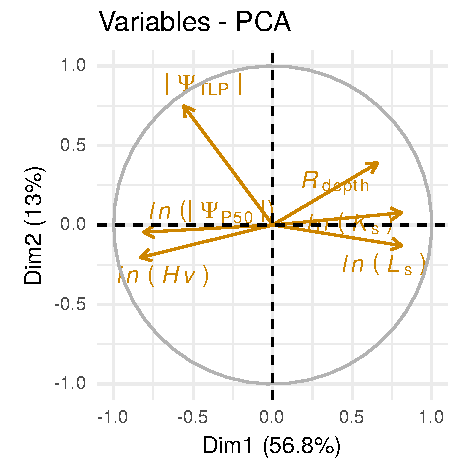
\includegraphics{figure/appendixD/figpca} 

}

\caption{PCA plot of water relations traits using imputations. $ln(|\Psi_{\text{P50}}|)$: logarithm of absolute water potential at 50\% water conductivity loss; $ln(K_{\text{s}})$: logarithm of maximum sapwood water conductivity; $ln(Hv)$: logarithm of Huber value; $|\Psi_{\text{TLP}}|$: absolute water potential at turgor-loss point; $R_{\text{depth}}$: rooting depth; $ln(L_{\text{s}})$: logarithm of individual leaf area.}\label{fig:unnamed-chunk-14}
\end{figure}
\newgeometry{layout=a4paper,left=1in,right=0.2in,top=0.2in,bottom=0.2in,nohead}
\begin{landscape}
\begin{figure}[H]

{\centering 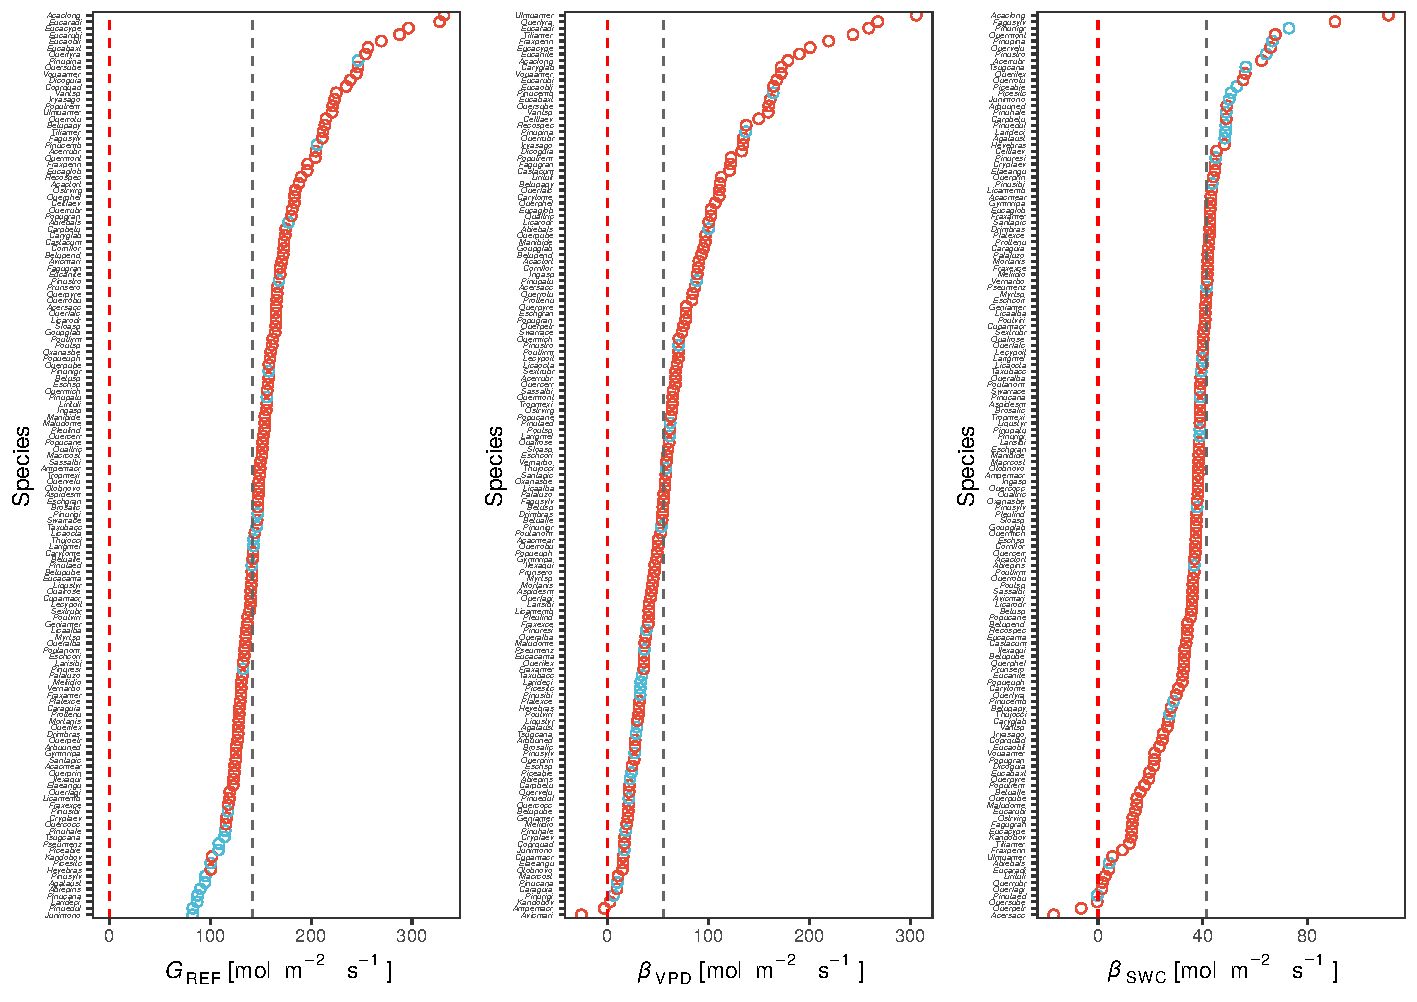
\includegraphics{figure/appendixD/fig17} 

}

\caption{Water use parameters at the species level. Grey dashed lines are the weighted mean of the parameters}\label{fig:spparamplot}
\end{figure}

\end{landscape}
\restoregeometry
\begin{figure}[H]

{\centering 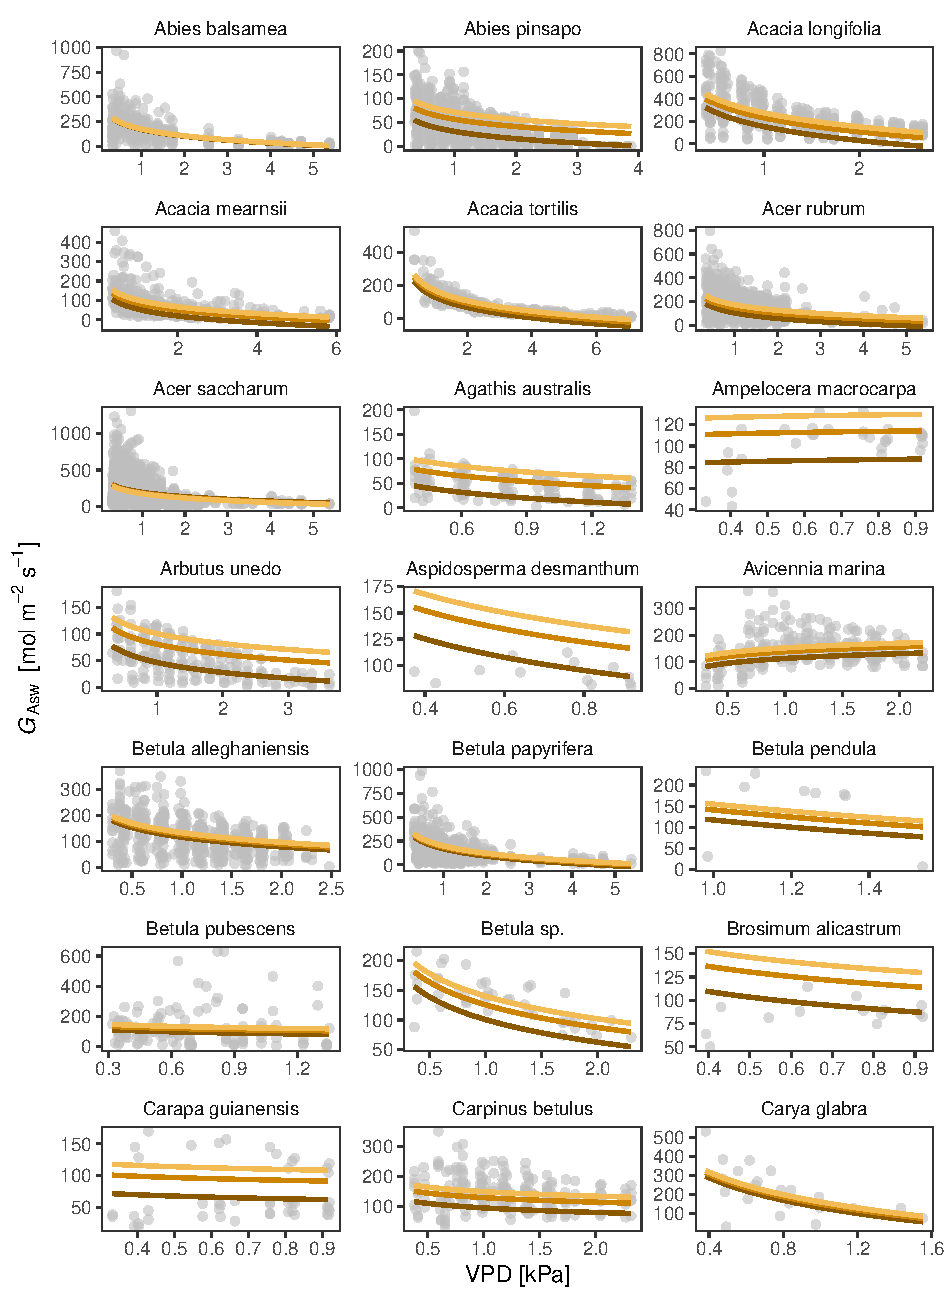
\includegraphics[width=1\linewidth]{figure/appendixD/ggg1} 

}

\end{figure}
\begin{figure}[H]

{\centering 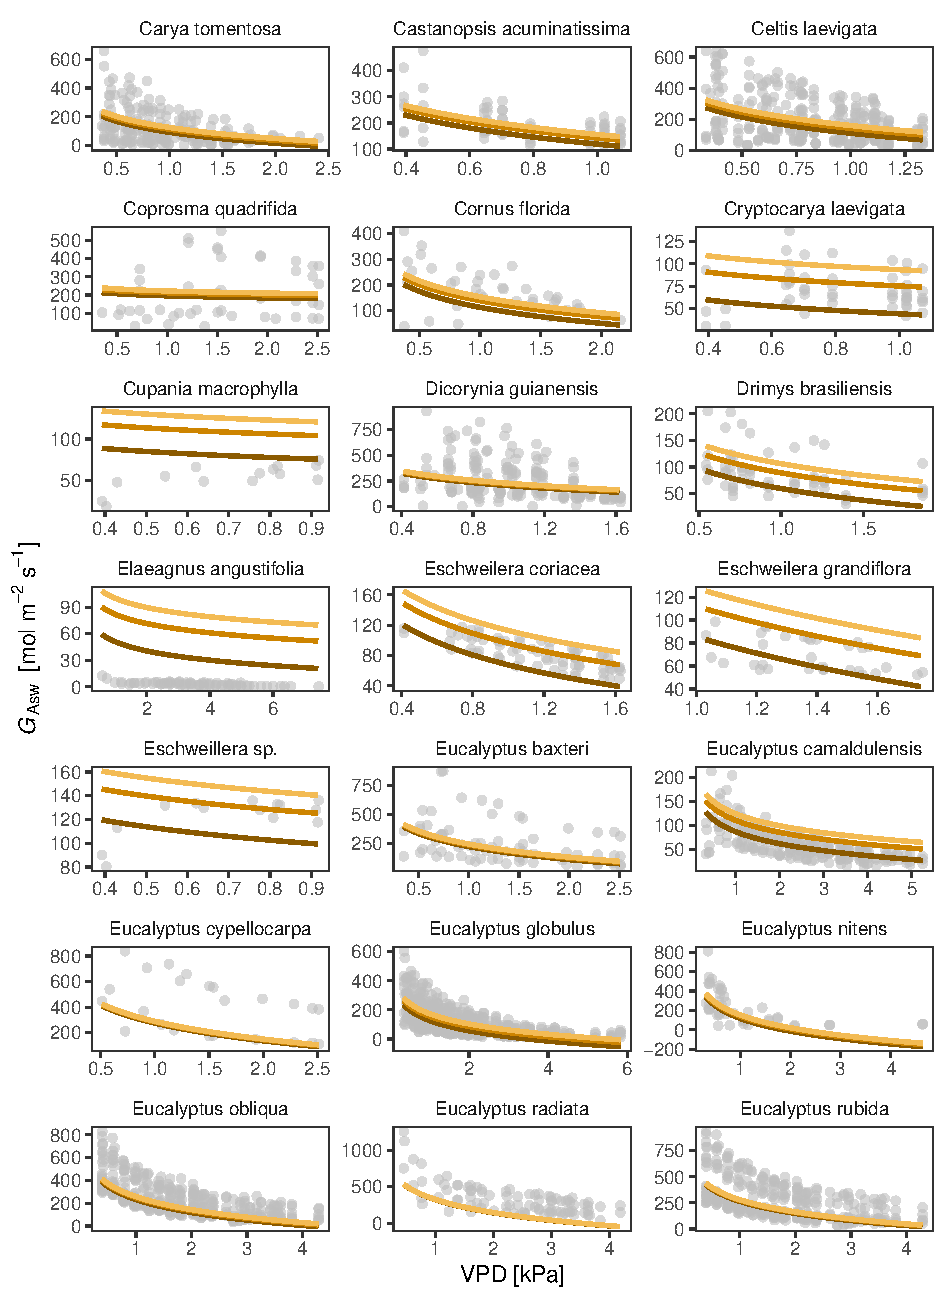
\includegraphics[width=1\linewidth]{figure/appendixD/ggg2} 

}

\end{figure}
\begin{figure}[H]

{\centering 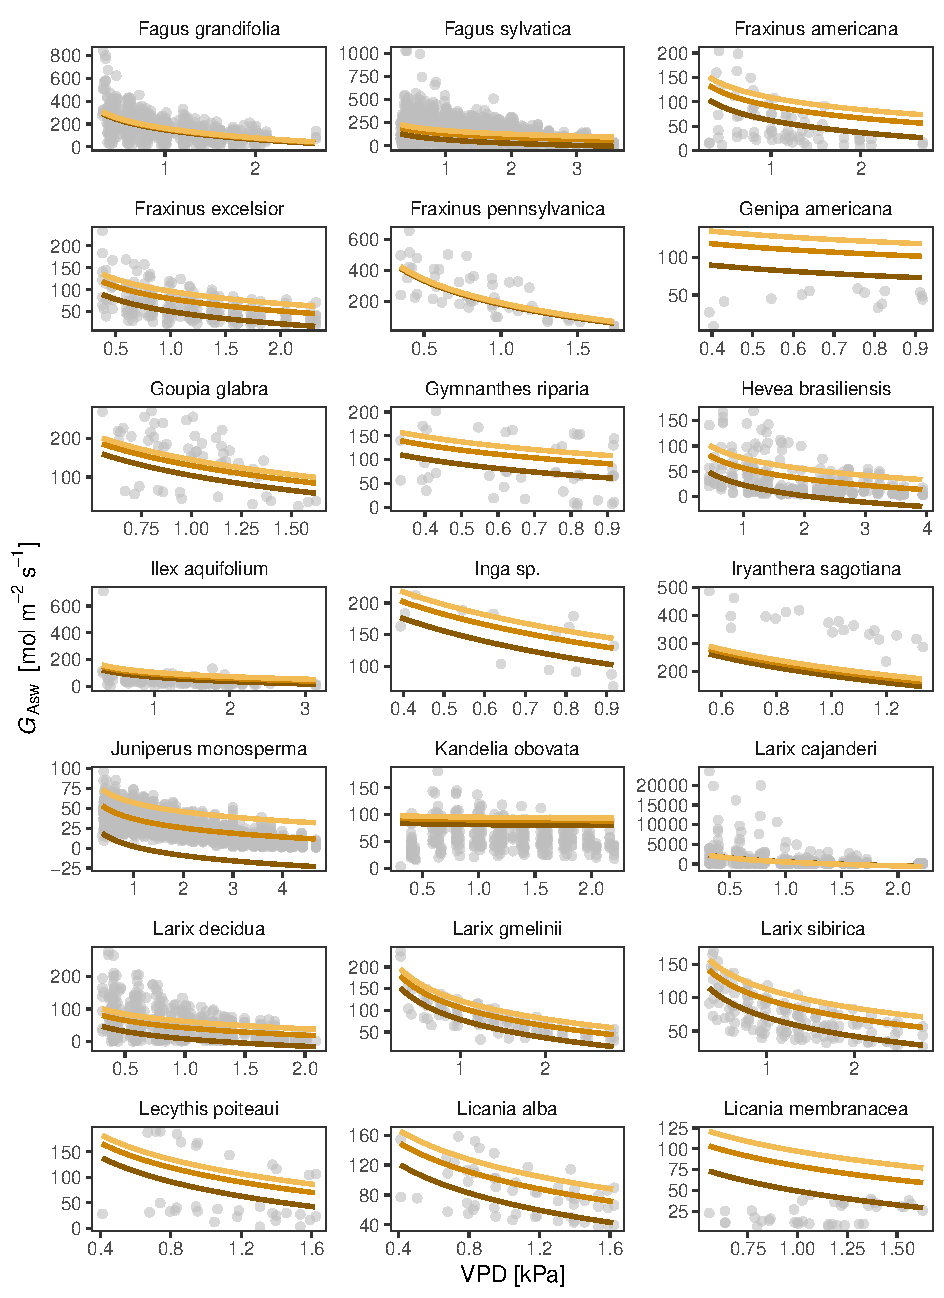
\includegraphics[width=1\linewidth]{figure/appendixD/ggg3} 

}

\end{figure}
\begin{figure}[H]

{\centering 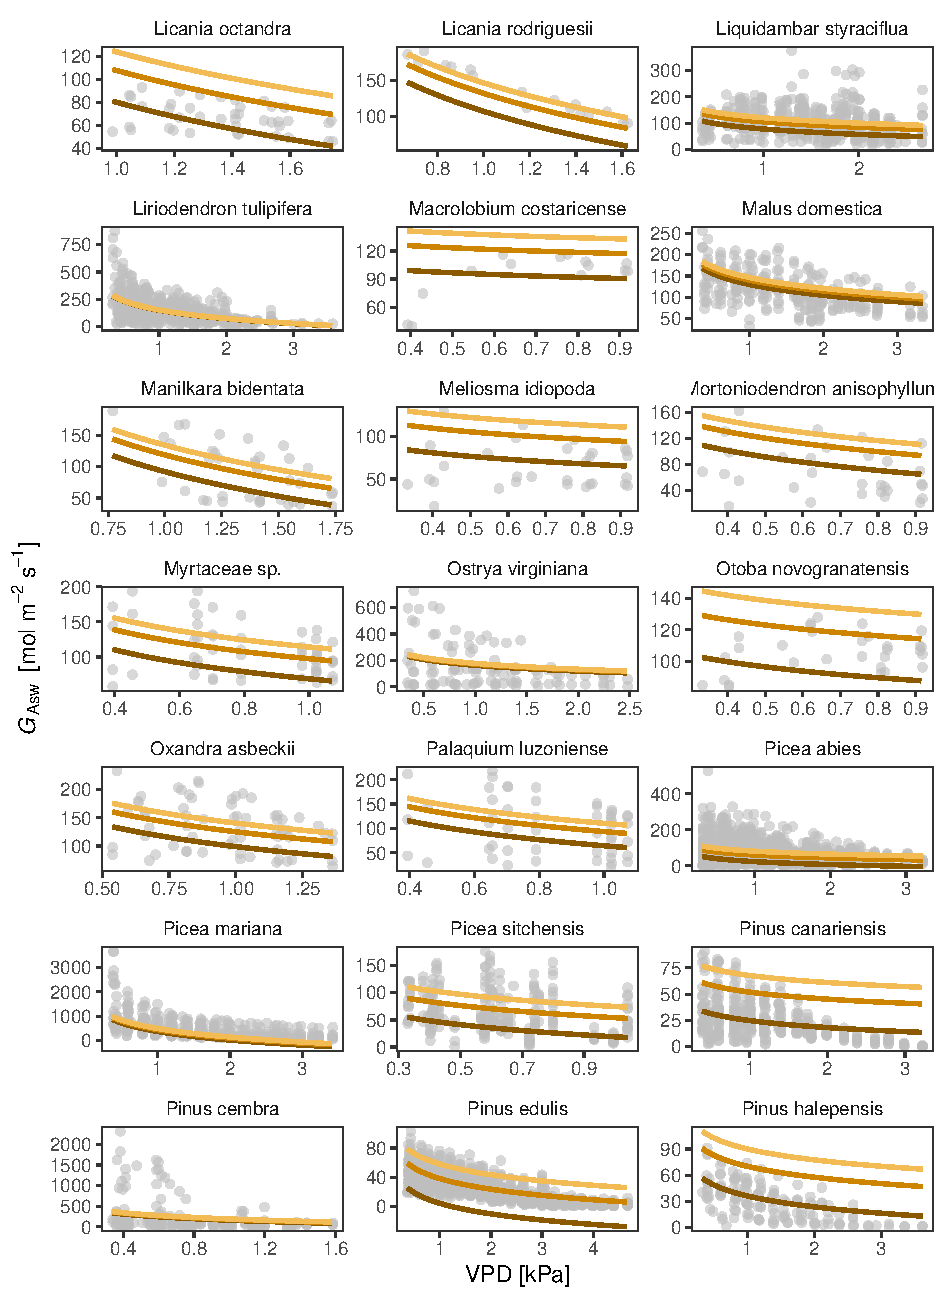
\includegraphics[width=1\linewidth]{figure/appendixD/ggg4} 

}

\end{figure}
\begin{figure}[H]

{\centering 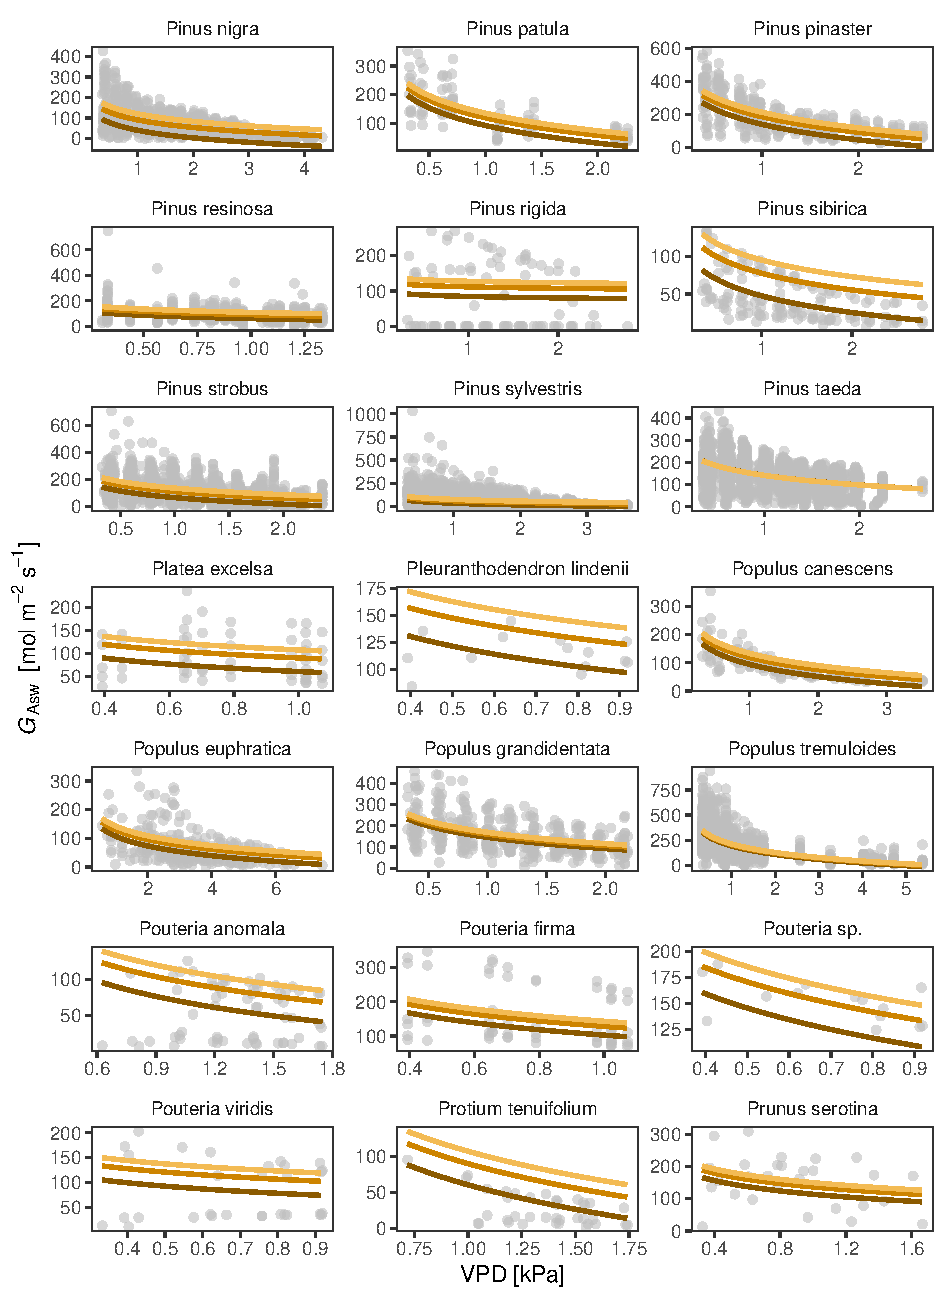
\includegraphics[width=1\linewidth]{figure/appendixD/ggg5} 

}

\end{figure}
\begin{figure}[H]

{\centering 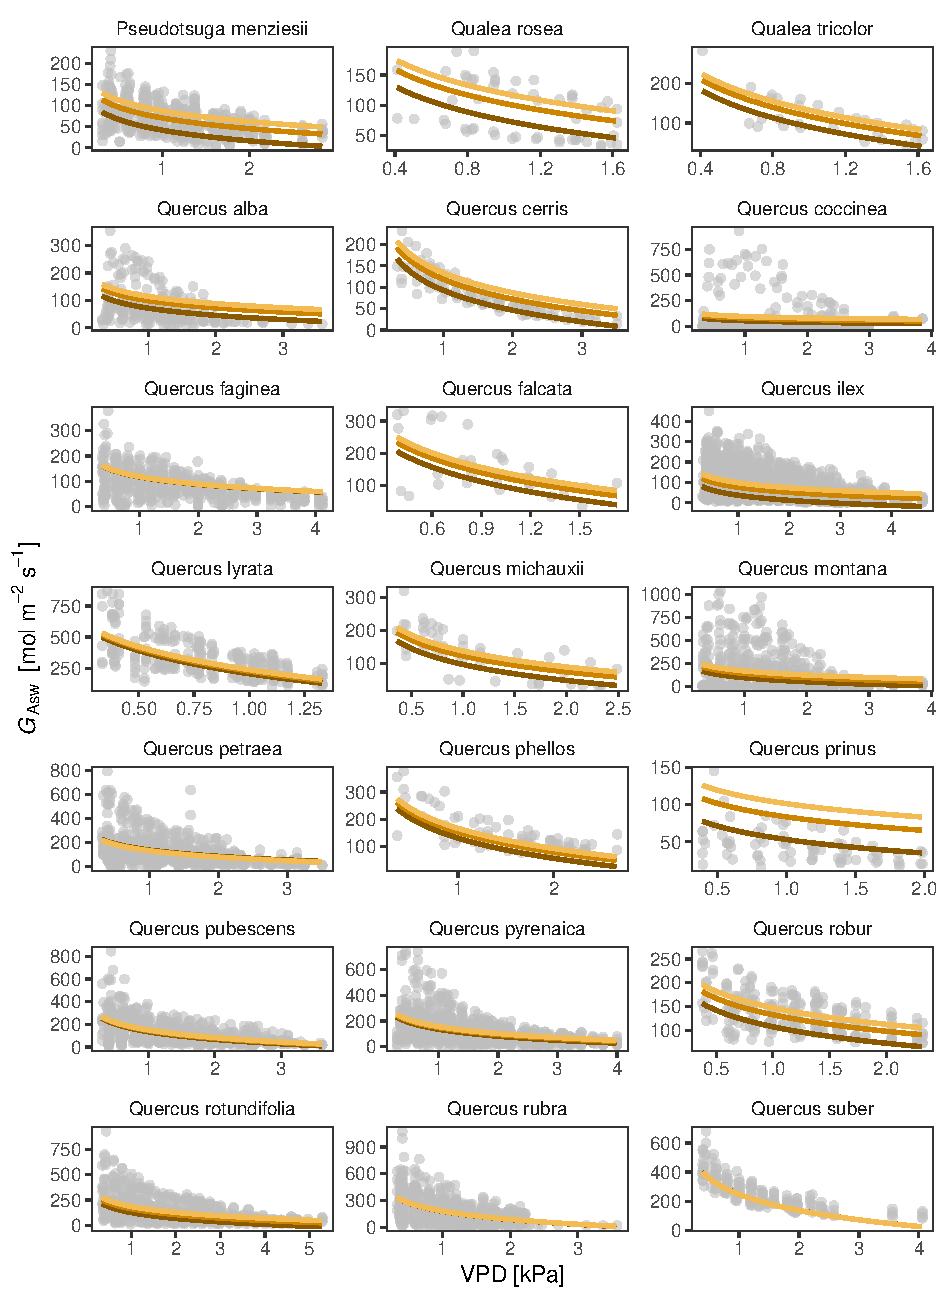
\includegraphics[width=1\linewidth]{figure/appendixD/ggg6} 

}

\end{figure}
\begin{figure}[H]

{\centering 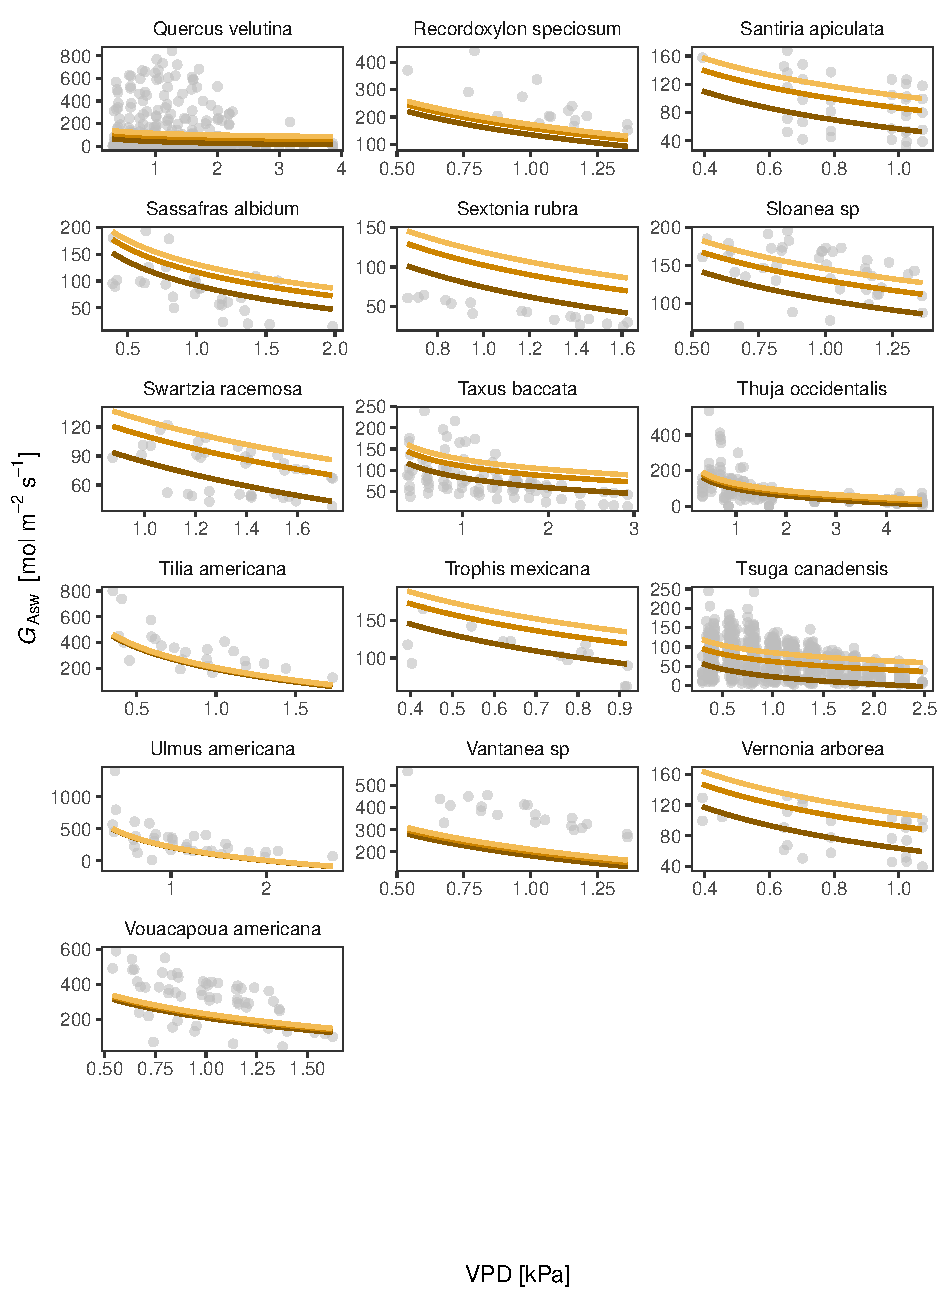
\includegraphics[width=1\linewidth]{figure/appendixD/ggg7} 

}

\caption{Species $G_{Asw}$ responses to VPD. Each species have different curves representing distinct levels of SWC (from dark to light, 0.1, 0.2, 0.3 [$m^3 m^{-3}$]).}\label{fig:unnamed-chunk-21}
\end{figure}
\begin{figure}[H]

{\centering 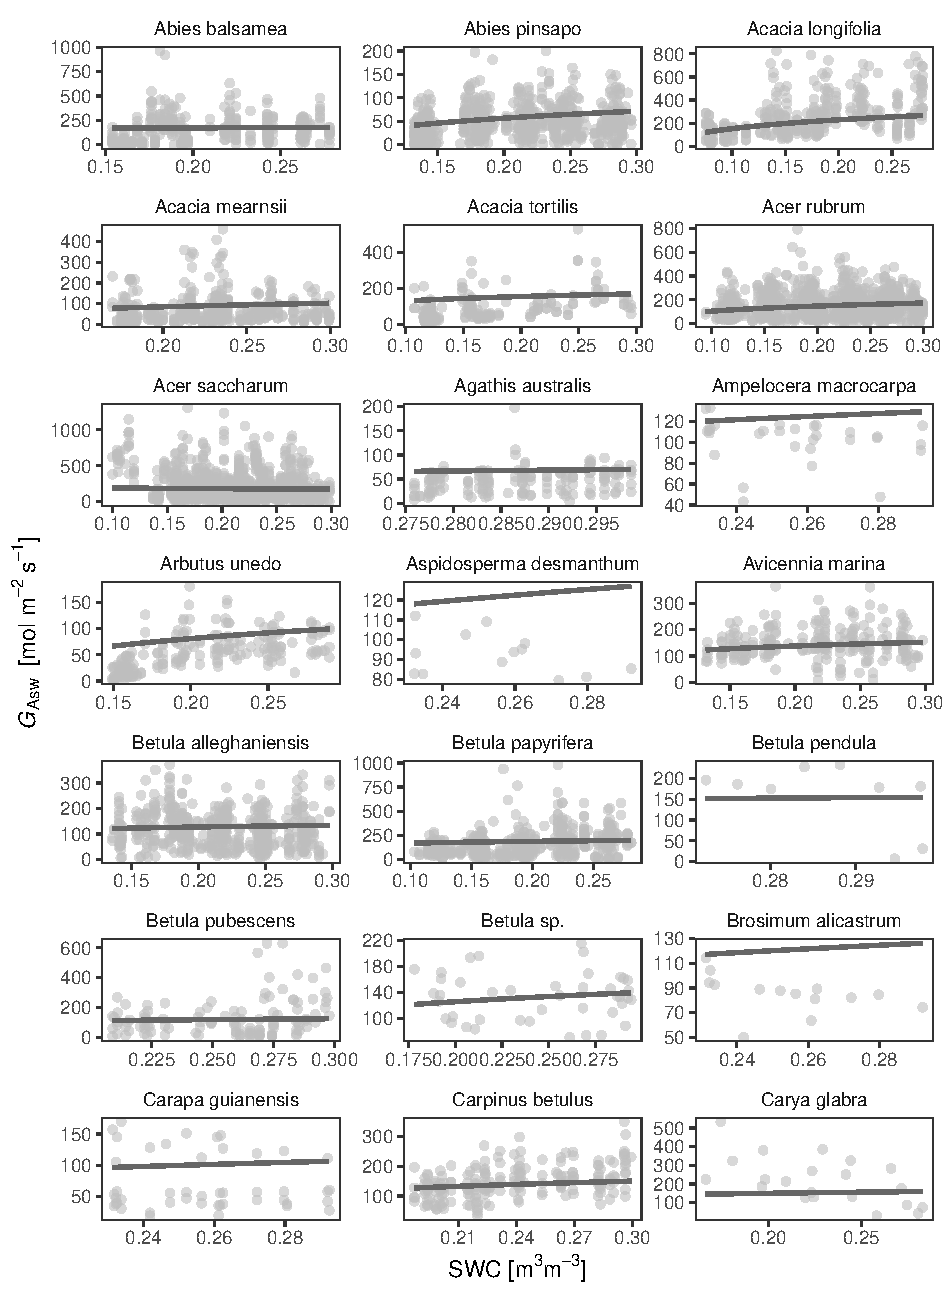
\includegraphics[width=1\linewidth]{figure/appendixD/ggg9} 

}

\end{figure}
\begin{figure}[H]

{\centering 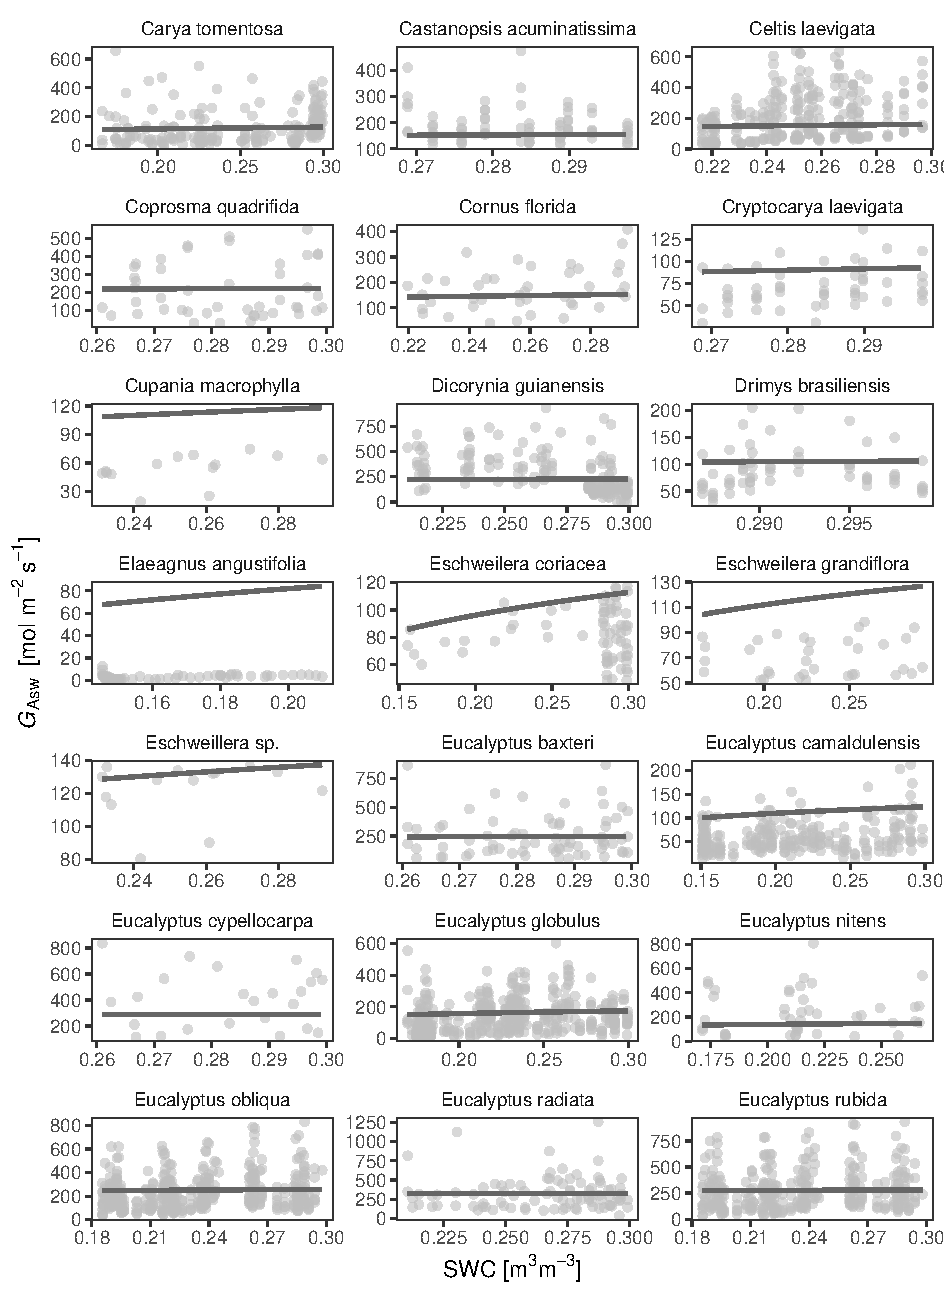
\includegraphics[width=1\linewidth]{figure/appendixD/ggg10} 

}

\end{figure}
\begin{figure}[H]

{\centering 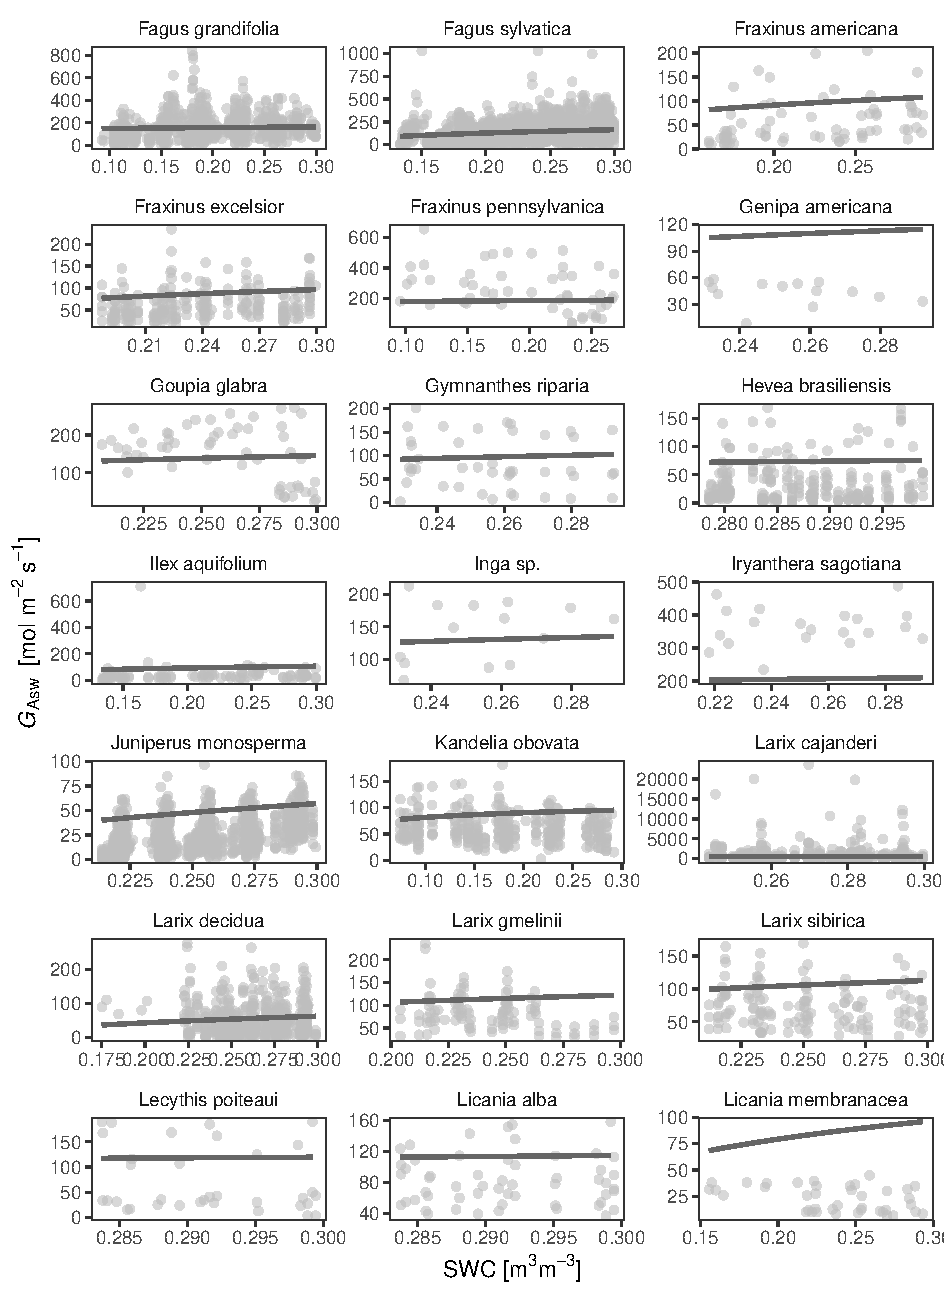
\includegraphics[width=1\linewidth]{figure/appendixD/ggg11} 

}

\end{figure}
\begin{figure}[H]

{\centering 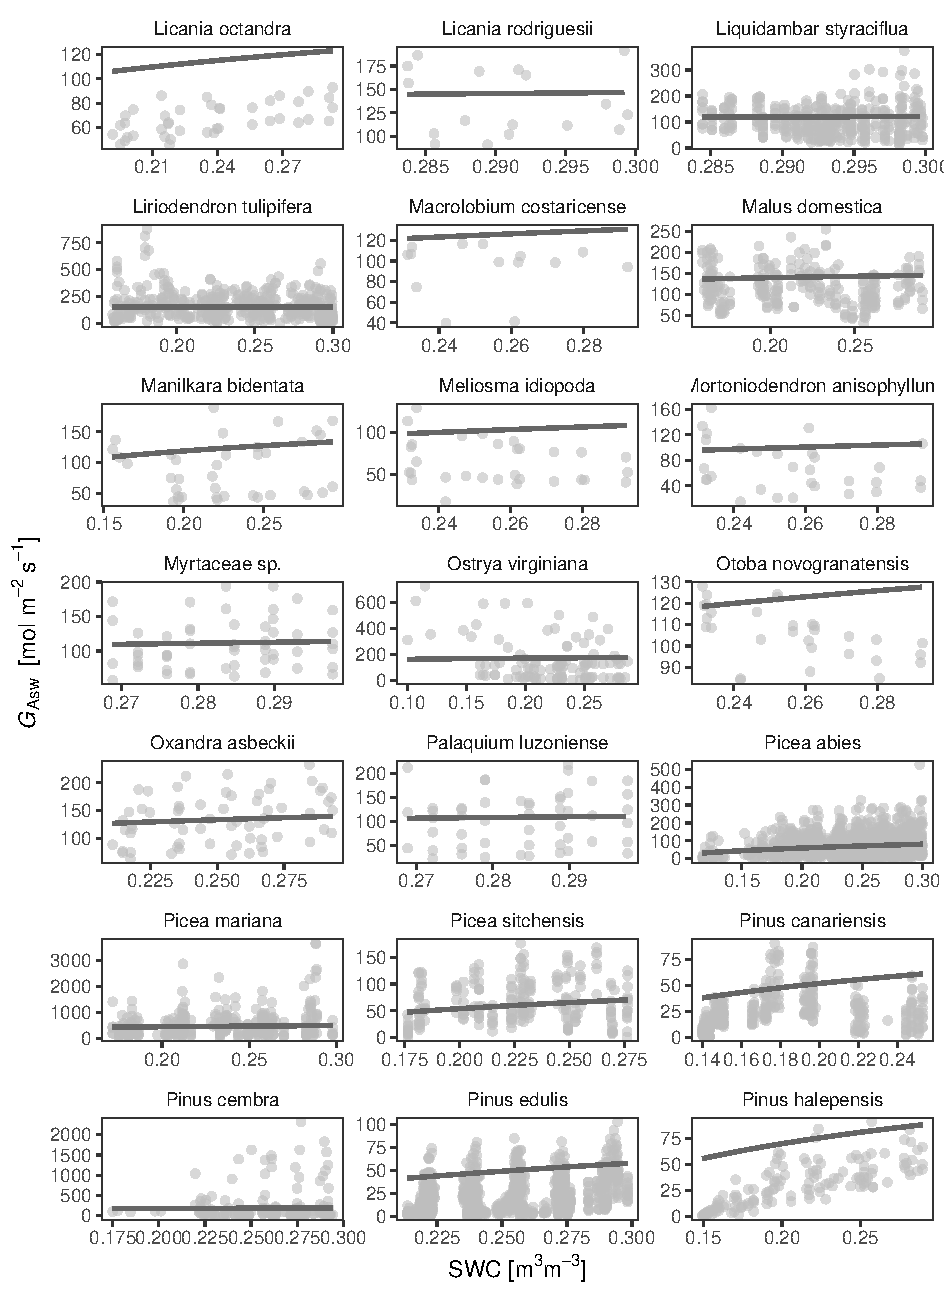
\includegraphics[width=1\linewidth]{figure/appendixD/ggg12} 

}

\end{figure}
\begin{figure}[H]

{\centering 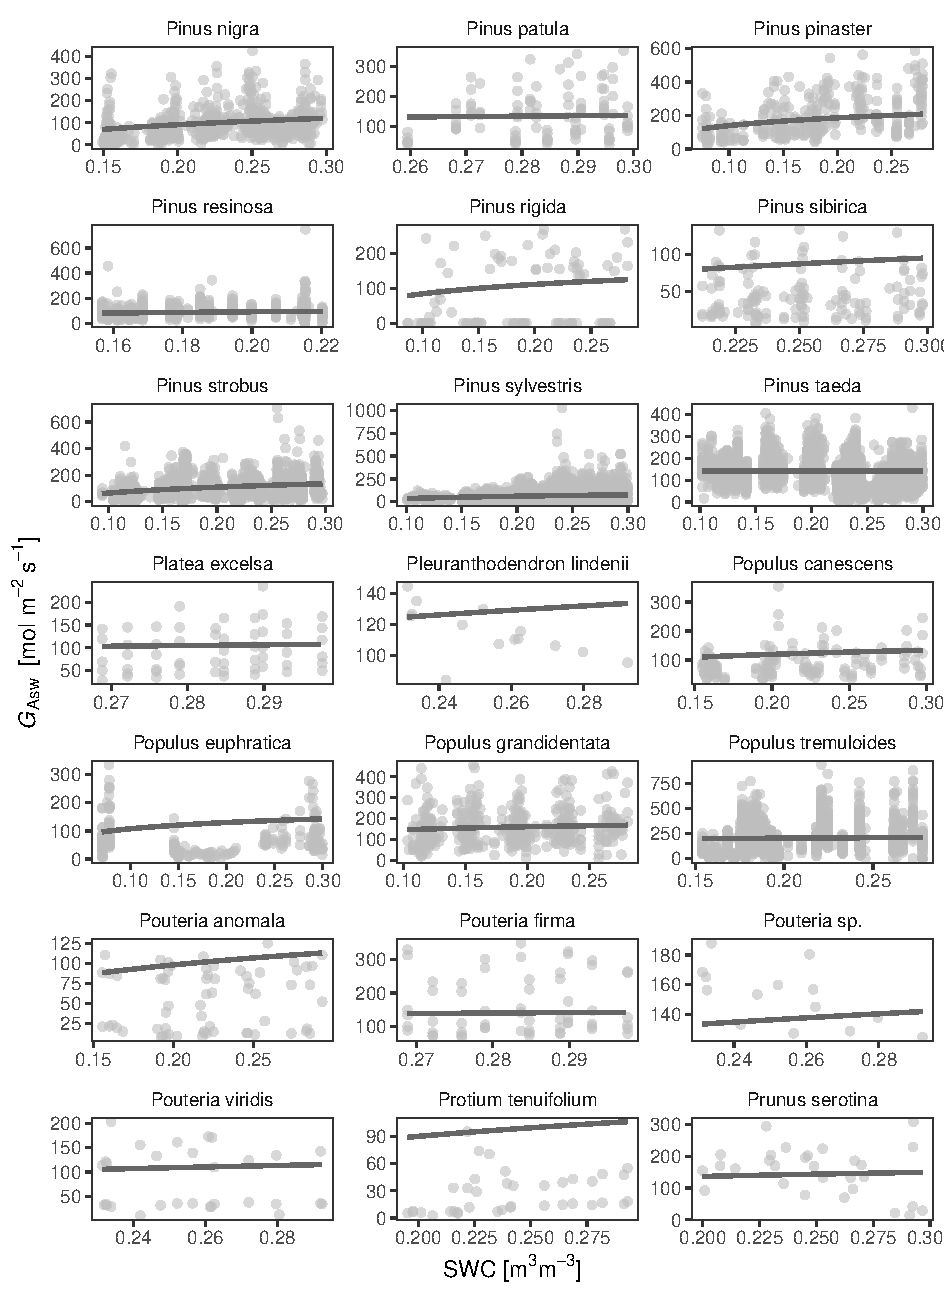
\includegraphics[width=1\linewidth]{figure/appendixD/ggg13} 

}

\end{figure}
\begin{figure}[H]

{\centering 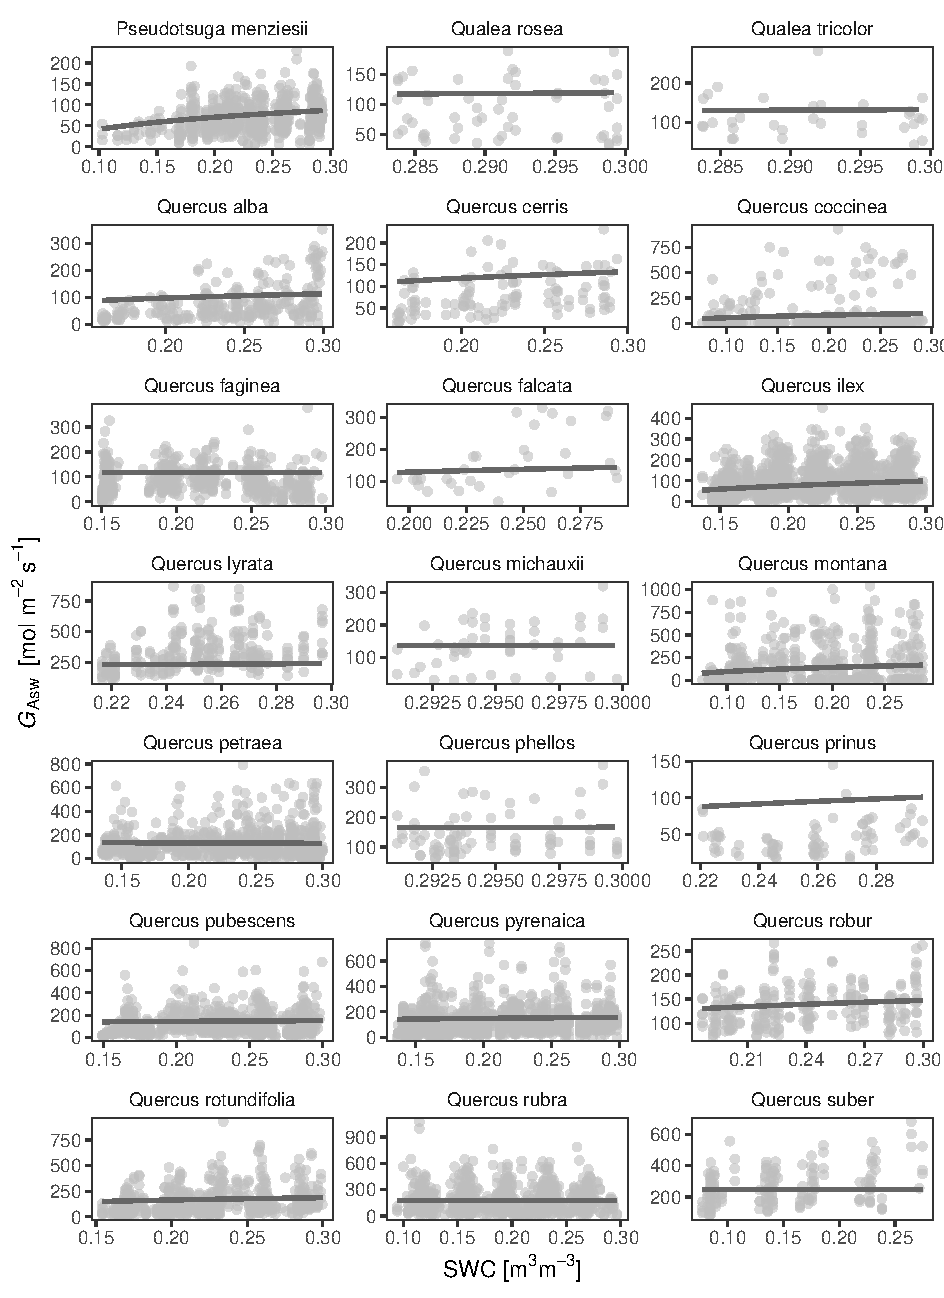
\includegraphics[width=1\linewidth]{figure/appendixD/ggg14} 

}

\end{figure}
\begin{figure}[H]

{\centering 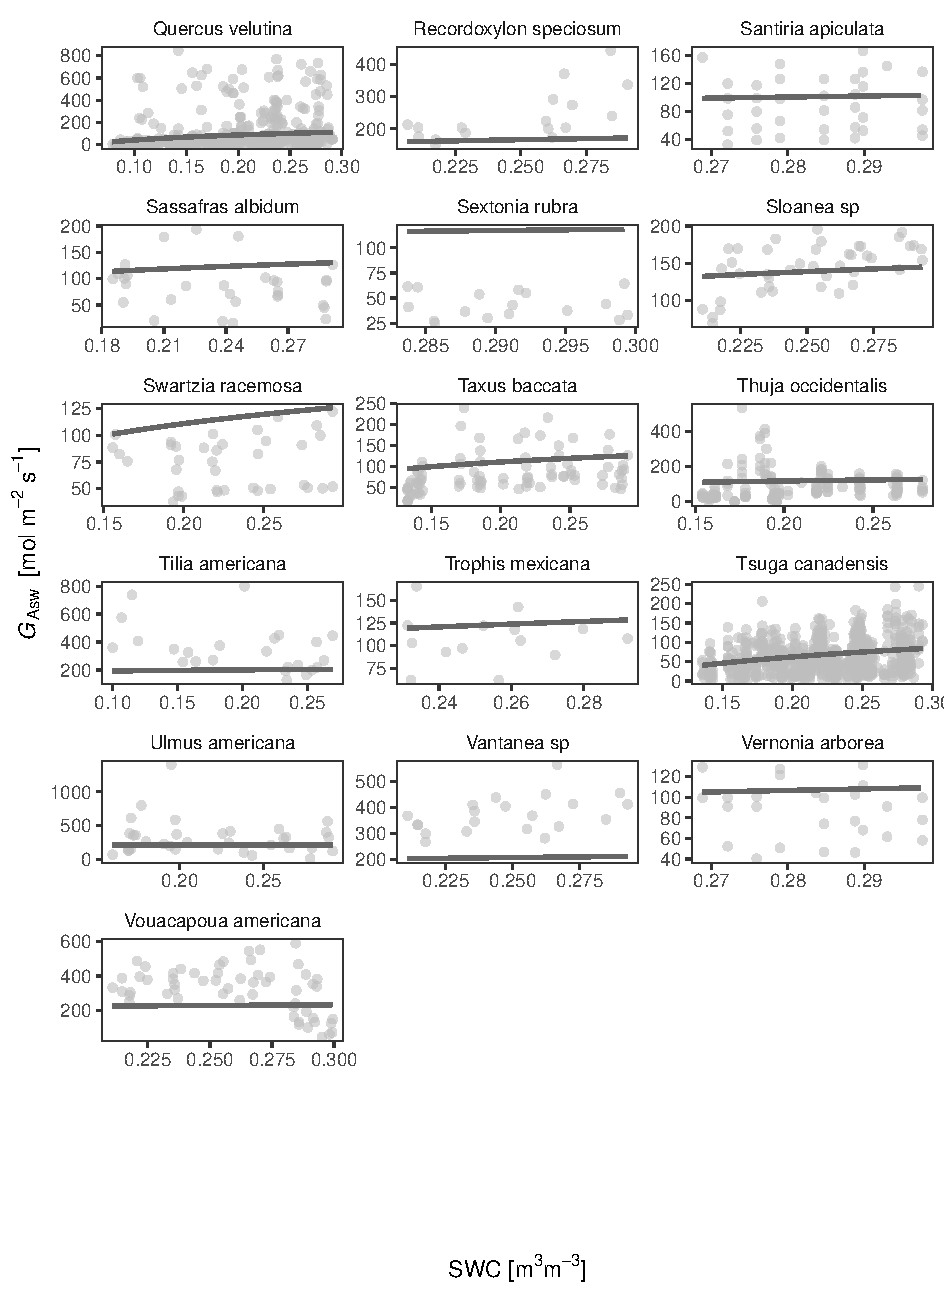
\includegraphics[width=1\linewidth]{figure/appendixD/ggg15} 

}

\caption{Species $G_{Asw}$ responses to SWC. Curves are fitted using a VPD reference level of 1 kPa.}\label{fig:unnamed-chunk-28}
\end{figure}
\begin{figure}[H]

{\centering 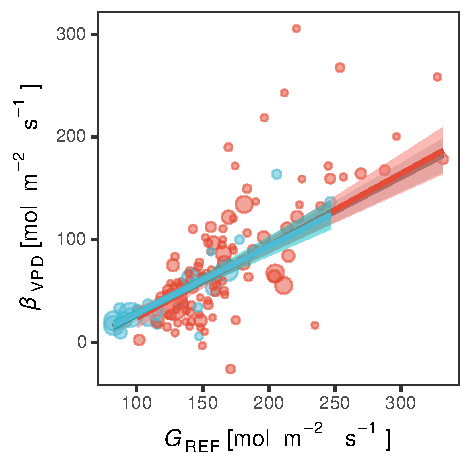
\includegraphics[width=1\linewidth]{figure/appendixD/fig_Gref_b1} 

}

\caption{Scatterplot between $G_{\text{REF}}$ and $\beta_{\text{VPD}}$ parameters. Grey line is global relationship. Blue and red lines are angiosperms and gymnosperms relationships, respectively. Shadow areas are 95\% confidence interval.}\label{fig:corrplot}
\end{figure}
\begin{figure}[H]

{\centering 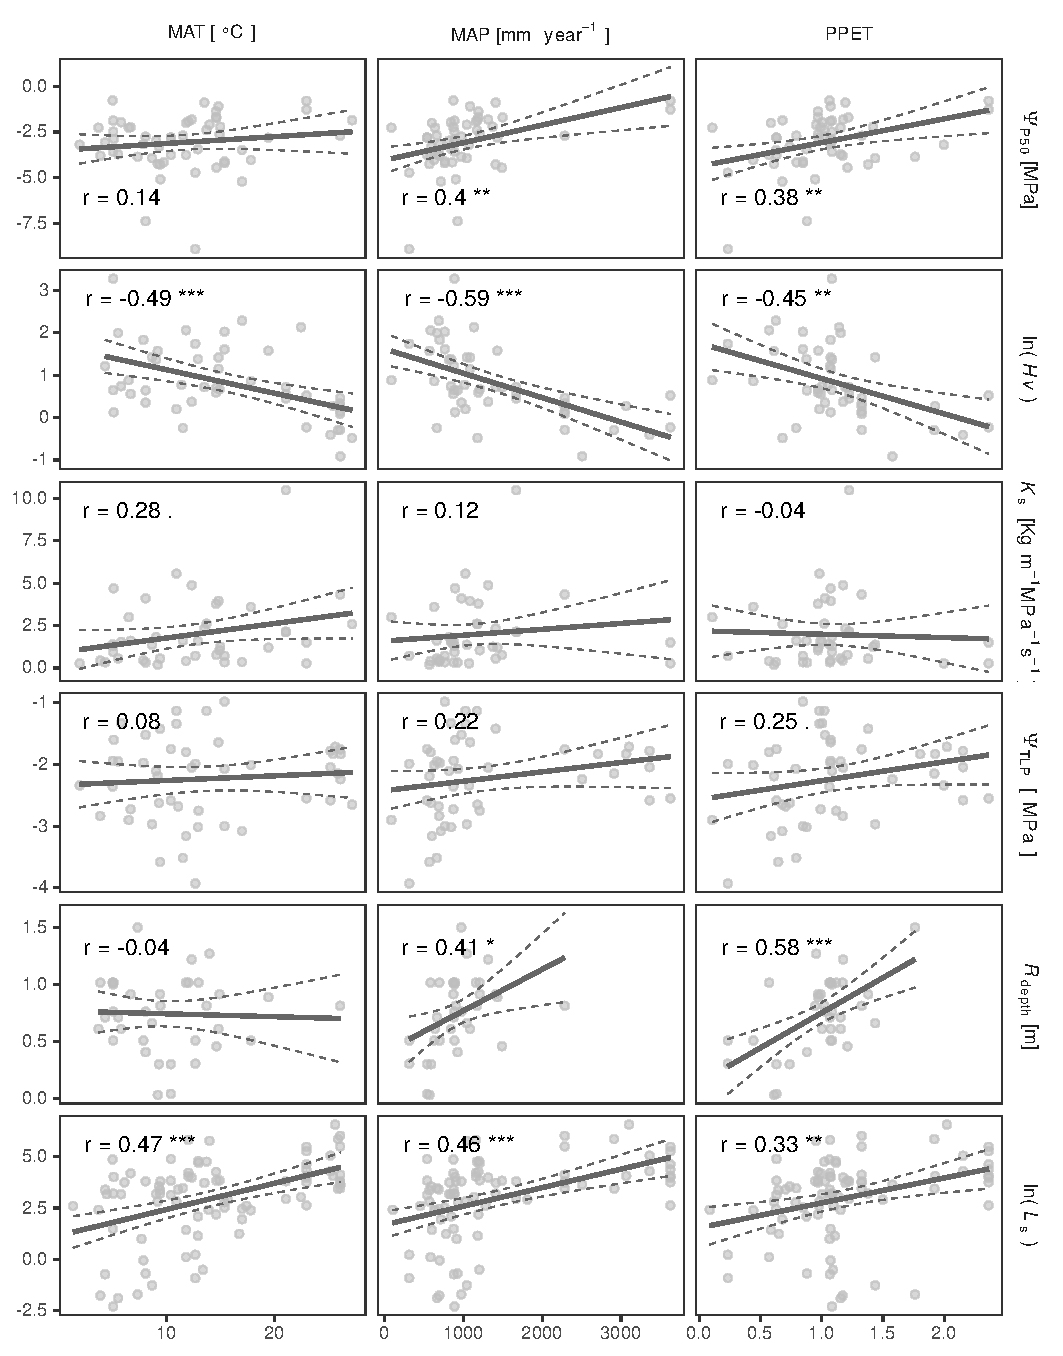
\includegraphics[width=1\linewidth]{figure/appendixD/fig7} 

}

\caption{Species' climatic variables and water relations traits relationships. MAP: mean annual precipitation, MAT: mean annual temperature, PPET: mean annual precipitation over potential evapotranspiration. All climatic variables were calculated as the weighted average of the characteristic plots of the trees of each species, using tree-days as weighting factor.}\label{fig:climatetraitsplot}
\end{figure}
\begin{figure}[H]

{\centering 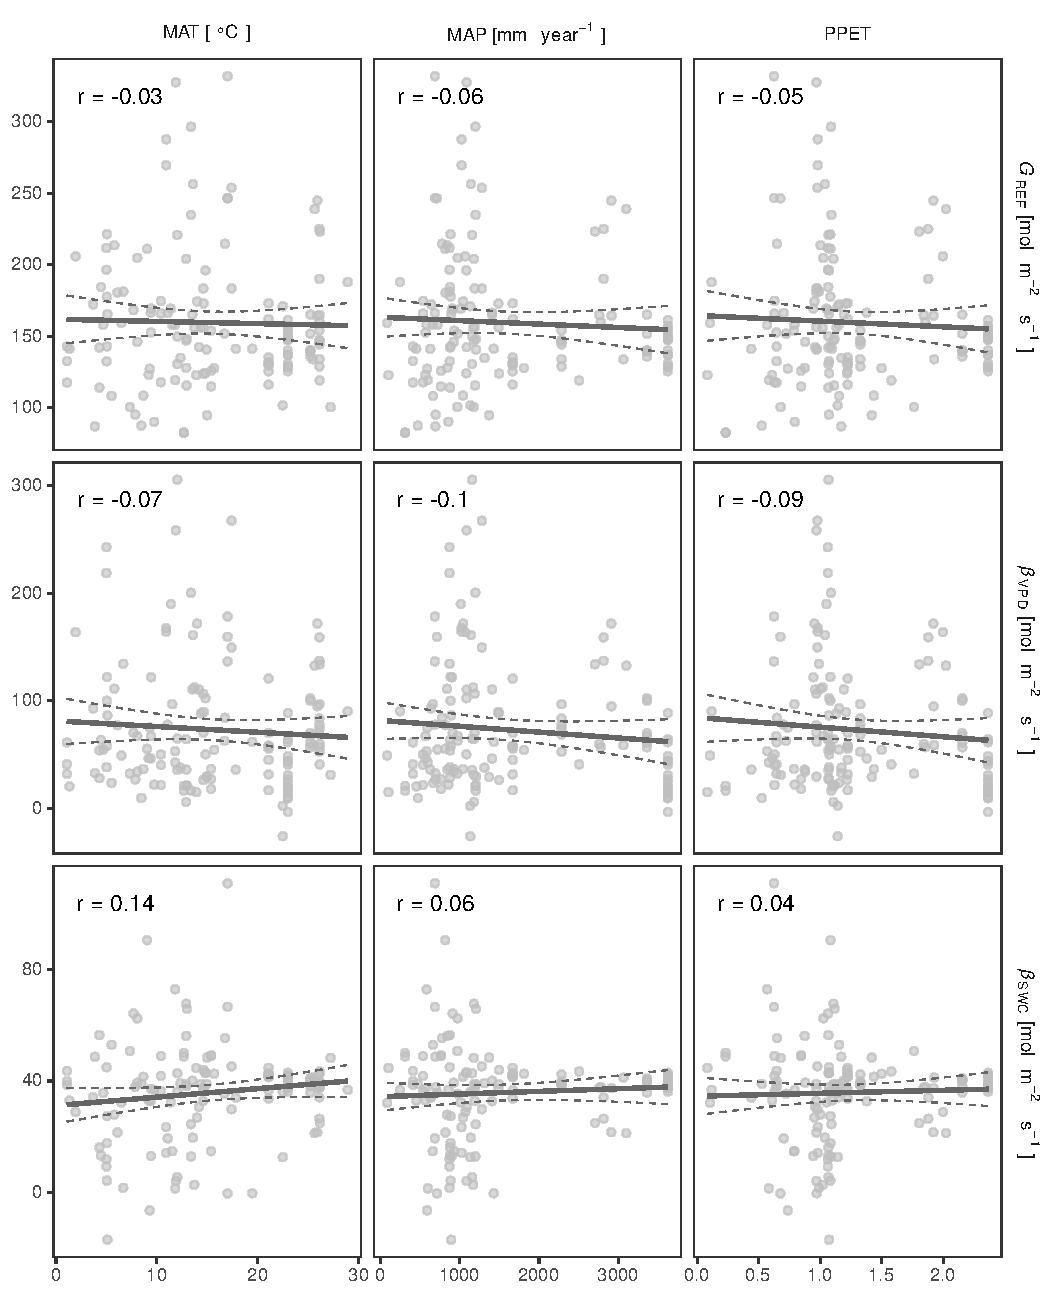
\includegraphics[width=1\linewidth]{figure/appendixD/fig22} 

}

\caption{Species' climatic variables and water use parameters relationships. MAP: mean annual precipitation, MAT: mean annual temperature, PPET: mean annual precipitation over potential evapotranspiration. All climatic variables were calculated as the weighted average of the characteristic plots of the trees of each species, using tree-days as weighting factor.}\label{fig:climateparamplot}
\end{figure}
\begin{figure}[H]

{\centering 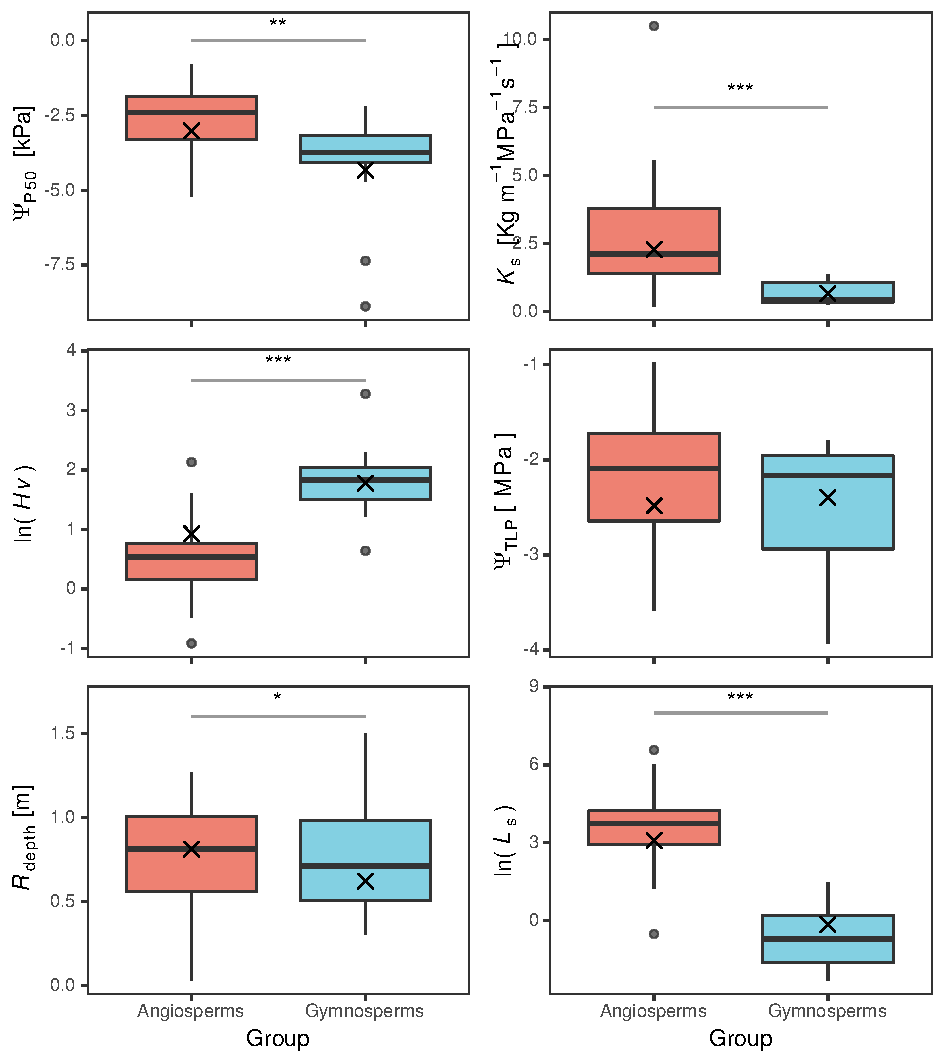
\includegraphics[width=1\linewidth]{figure/appendixD/figanggym} 

}

\caption{Boxplots of water relations traits for angiosperms and gymnosperms. Statistical significance level is showed as symbols: ., P < 0.1; *, P < 0.05; **, P < 0.01; ***, P < 0.001. Crosses are weighted means of each trait by groups}\label{fig:angiogymnoplotsAOVplot}
\end{figure}
\newpage

\section{Tables D}\label{tables-d}
\begin{table}[H]

\caption{\label{tab:plottreatment}SAPFLUXNET plot treatments included in this study (Poyatos $et al.$ 2020).}
\centering
\begin{tabular}[t]{l}
\toprule
Plot treatment\\
\midrule
\\
None\\
Control\\
control\\
Ambient Control\\
Control - Unthinned\\
natural conditions\\
Reference\\
1Premortality\\
2premortality\\
distructive sampling\\
Girdling early successional\\
Pre-thinning\\
Before thinning\\
Before Thinning\\
non thinned\\
none (periodict thinning every 5-6 years  20 to 25\% of basal area)\\
Radiation Level\\
AMBIENT CO2 FACE rings\\
fertilization at plantation\\
AcaciaMonoculture\\
MixtureEucalyptusAndAcacia\\
EucalyptusMonoculture\\
Pre Irrigation\\
\bottomrule
\end{tabular}
\end{table}
\begingroup\fontsize{4.5}{6.5}\selectfont
\begin{longtable}[t]{>{\em\raggedright\arraybackslash}p{10em}>{\raggedright\arraybackslash}p{4em}>{\raggedright\arraybackslash}p{4em}>{\raggedleft\arraybackslash}p{3em}>{\raggedleft\arraybackslash}p{2em}>{\raggedleft\arraybackslash}p{2em}>{\raggedleft\arraybackslash}p{3em}>{\raggedleft\arraybackslash}p{3em}>{\raggedleft\arraybackslash}p{3em}>{\raggedleft\arraybackslash}p{3em}>{\raggedleft\arraybackslash}p{3em}>{\raggedleft\arraybackslash}p{3em}}
\caption{\label{tab:tabledata}Species resume table. CEP names are Cornell Ecology Programs species names. $\Psi_{\text{P50}}$: water potential at 50\% water conductivity loss [\text{$MPa$}]; $K_\text{s}$: maximum sapwood water conductivity[\text{$Kg\;m^{-1}\;MPa^{-1}\;s^{-1}$}]; $Hv$: Huber value [\text{$cm^2_{Asw}\;m^{-2}_{leaf\;area}$}]; $\Psi_{\text{TLP}}$: water potential at turgor-loss point[\text{$MPa$}]; $R_{\text{depth}}$: rooting depth [\text{$m$}]; $L_{\text{s}}$: individual leaf area [\text{$cm^2$}].}\\
\toprule
\rotatebox{45}{$\text{Species}$} & \rotatebox{45}{$\text{CEP names}$} & \rotatebox{45}{$\text{Group}$} & \rotatebox{45}{$\# \; \text{tree-days}$} & \rotatebox{45}{$\# \; \text{trees}$} & \rotatebox{45}{$\# \; \text{plots}$} & \rotatebox{45}{$\Psi_{\text{P50}}$} & \rotatebox{45}{$K_{\text{s}}$} & \rotatebox{45}{$\Psi_{\text{TLP}}$} & \rotatebox{45}{$Hv$} & \rotatebox{45}{$R_{\text{depth}}$} & \rotatebox{45}{$L_{\text{s}}$}\\
\midrule
\endfirsthead
\caption[]{\label{tab:tabledata}Species resume table. CEP names are Cornell Ecology Programs species names. $\Psi_{\text{P50}}$: water potential at 50\% water conductivity loss [\text{$MPa$}]; $K_\text{s}$: maximum sapwood water conductivity[\text{$Kg\;m^{-1}\;MPa^{-1}\;s^{-1}$}]; $Hv$: Huber value [\text{$cm^2_{Asw}\;m^{-2}_{leaf\;area}$}]; $\Psi_{\text{TLP}}$: water potential at turgor-loss point[\text{$MPa$}]; $R_{\text{depth}}$: rooting depth [\text{$m$}]; $L_{\text{s}}$: individual leaf area [\text{$cm^2$}]. \textit{(continued)}}\\
\toprule
\rotatebox{45}{$\text{Species}$} & \rotatebox{45}{$\text{CEP names}$} & \rotatebox{45}{$\text{Group}$} & \rotatebox{45}{$\# \; \text{tree-days}$} & \rotatebox{45}{$\# \; \text{trees}$} & \rotatebox{45}{$\# \; \text{plots}$} & \rotatebox{45}{$\Psi_{\text{P50}}$} & \rotatebox{45}{$K_{\text{s}}$} & \rotatebox{45}{$\Psi_{\text{TLP}}$} & \rotatebox{45}{$Hv$} & \rotatebox{45}{$R_{\text{depth}}$} & \rotatebox{45}{$L_{\text{s}}$}\\
\midrule
\endhead
\
\endfoot
\bottomrule
\endlastfoot
Abies balsamea & Abiebals & Gymnosperms & 855 & 19 & 1 & -2.479 & 1.292 &  & 26.600 & 0.508 & \\
Abies pinsapo & Abiepins & Gymnosperms & 11822 & 22 & 3 & -4.150 &  &  &  &  & \\
Acacia longifolia & Acaclong & Angiosperms & 2130 & 10 & 1 &  &  &  &  &  & 11.715\\
Acacia mearnsii & Acacmear & Angiosperms & 4555 & 23 & 2 &  &  &  & 4.134 &  & \\
Acacia tortilis & Acactort & Angiosperms & 1740 & 3 & 1 &  &  &  &  &  & \\
Acer rubrum & Acerrubr & Angiosperms & 17230 & 49 & 9 & -2.755 & 4.108 & -1.520 & 1.422 & 0.762 & 44.983\\
Acer saccharum & Acersacc & Angiosperms & 10928 & 156 & 8 & -2.873 & 4.695 & -1.600 & 1.134 & 1.016 & 55.675\\
Agathis australis & Agataust & Gymnosperms & 1272 & 6 & 1 & -2.210 & 1.250 &  &  &  & \\
Ampelocera macrocarpa & Ampemacr & Angiosperms & 100 & 2 & 1 &  &  &  &  &  & 103.560\\
Arbutus unedo & Arbuuned & Angiosperms & 1900 & 4 & 1 & -4.198 & 0.714 & -0.980 & 5.017 &  & 12.470\\
Aspidosperma desmanthum & Aspidesm & Angiosperms & 35 & 1 & 1 &  &  &  &  &  & 42.925\\
Avicennia marina & Avicmari & Angiosperms & 828 & 6 & 1 &  &  &  & 8.435 &  & 20.800\\
Betula alleghaniensis & Betualle & Angiosperms & 3750 & 16 & 2 &  &  &  &  &  & 29.938\\
Betula papyrifera & Betupapy & Angiosperms & 3869 & 21 & 2 & -1.966 & 1.538 & -1.330 & 2.096 & 0.610 & 23.942\\
Betula pendula & Betupend & Angiosperms & 9 & 1 & 1 & -2.265 &  &  &  & 0.610 & 11.177\\
Betula pubescens & Betupube & Angiosperms & 397 & 9 & 2 &  &  &  &  &  & 13.510\\
Betula sp. & Betusp & Angiosperms & 204 & 2 & 1 &  &  &  &  &  & \\
Brosimum alicastrum & Brosalic & Angiosperms & 40 & 1 & 1 &  &  &  & 1.685 &  & 58.953\\
Carapa guianensis & Caraguia & Angiosperms & 150 & 3 & 1 & -0.800 & 0.270 &  & 0.793 &  & \\
Carpinus betulus & Carpbetu & Angiosperms & 530 & 5 & 1 & -3.750 &  &  &  &  & 23.160\\
Carya glabra & Caryglab & Angiosperms & 47 & 1 & 1 & -2.100 &  &  &  & 1.270 & 324.425\\
Carya tomentosa & Carytome & Angiosperms & 645 & 10 & 2 &  &  &  &  &  & \\
Castanopsis acuminatissima & Castacum & Angiosperms & 96 & 8 & 1 &  & 10.490 &  & 1.570 &  & 45.000\\
Celtis laevigata & Celtlaev & Angiosperms & 745 & 13 & 2 &  &  &  &  &  & 13.580\\
Coprosma quadrifida & Coprquad & Angiosperms & 57 & 4 & 2 &  &  &  &  &  & 0.600\\
Cornus florida & Cornflor & Angiosperms & 126 & 1 & 1 & -4.442 & 0.768 &  & 2.034 & 0.457 & 46.343\\
Cryptocarya laevigata & Cryplaev & Angiosperms & 72 & 6 & 1 &  & 2.140 &  & 1.750 &  & 19.075\\
Cupania macrophylla & Cupamacr & Angiosperms & 40 & 1 & 1 &  &  &  &  &  & \\
Dicorynia guianensis & Dicoguia & Angiosperms & 596 & 9 & 2 &  &  & -1.712 &  &  & 717.500\\
Drimys brasiliensis & Drimbras & Angiosperms & 90 & 5 & 1 &  &  &  &  &  & 18.420\\
Elaeagnus angustifolia & Elaeangu & Angiosperms & 402 & 2 & 1 &  &  &  &  &  & 11.200\\
Eschweilera coriacea & Eschcori & Angiosperms & 249 & 4 & 2 &  &  & -1.828 & 1.312 &  & 58.654\\
Eschweilera grandiflora & Eschgran & Angiosperms & 378 & 2 & 1 &  &  & -1.754 & 0.746 &  & 62.085\\
Eschweillera sp. & Eschsp & Angiosperms & 40 & 1 & 1 &  &  &  &  &  & \\
Eucalyptus baxteri & Eucabaxt & Angiosperms & 112 & 4 & 2 &  &  &  &  &  & \\
Eucalyptus camaldulensis & Eucacama & Angiosperms & 564 & 3 & 1 & -4.025 & 3.600 & -2.010 & 2.364 & 0.508 & 10.910\\
Eucalyptus cypellocarpa & Eucacype & Angiosperms & 29 & 2 & 2 &  &  &  &  &  & \\
Eucalyptus globulus & Eucaglob & Angiosperms & 4555 & 23 & 2 & -1.100 & 3.950 & -1.640 & 3.155 & 0.610 & \\
Eucalyptus nitens & Eucanite & Angiosperms & 378 & 7 & 1 &  &  &  & 2.163 &  & \\
Eucalyptus obliqua & Eucaobli & Angiosperms & 2466 & 6 & 1 &  &  & -1.340 &  &  & 16.790\\
Eucalyptus radiata & Eucaradi & Angiosperms & 170 & 2 & 1 &  &  &  &  &  & \\
Eucalyptus rubida & Eucarubi & Angiosperms & 2055 & 5 & 1 &  & 5.560 & -1.130 & 1.222 &  & \\
Fagus grandifolia & Fagugran & Angiosperms & 6815 & 32 & 3 & -5.080 &  &  &  & 0.813 & 45.167\\
Fagus sylvatica & Fagusylv & Angiosperms & 15075 & 93 & 12 & -2.972 & 1.830 & -2.107 & 3.934 &  & 24.030\\
Fraxinus americana & Fraxamer & Angiosperms & 378 & 2 & 1 & -1.920 &  &  &  & 1.016 & 339.552\\
Fraxinus excelsior & Fraxexce & Angiosperms & 636 & 6 & 1 & -2.805 &  & -1.750 &  & 0.040 & 133.800\\
Fraxinus pennsylvanica & Fraxpenn & Angiosperms & 178 & 2 & 1 & -0.777 & 1.397 & -2.360 &  & 1.016 & \\
Genipa americana & Geniamer & Angiosperms & 40 & 1 & 1 & -1.270 & 1.500 & -2.550 &  &  & 242.210\\
Goupia glabra & Goupglab & Angiosperms & 172 & 3 & 3 &  &  &  &  &  & 31.288\\
Gymnanthes riparia & Gymnripa & Angiosperms & 150 & 3 & 1 &  &  &  &  &  & \\
Hevea brasiliensis & Hevebras & Angiosperms & 1302 & 6 & 1 & -1.859 & 2.582 & -2.650 & 0.618 &  & \\
Ilex aquifolium & Ilexaqui & Angiosperms & 567 & 3 & 1 & -4.241 & 0.186 & -2.190 & 4.825 & 0.030 & 16.770\\
Inga sp. & Ingasp & Angiosperms & 40 & 1 & 1 &  &  &  &  &  & \\
Iryanthera sagotiana & Iryasago & Angiosperms & 72 & 1 & 1 &  &  & -1.830 &  &  & \\
Juniperus monosperma & Junimono & Gymnosperms & 23650 & 15 & 3 & -8.882 & 0.710 & -3.930 & 5.700 & 0.305 & 0.400\\
Kandelia obovata & Kandobov & Angiosperms & 2584 & 8 & 1 &  &  &  &  &  & \\
Larix decidua & Larideci & Gymnosperms & 3127 & 23 & 5 & -3.791 & 0.434 & -2.835 &  & 1.016 & 0.170\\
Larix gmelinii & Larigmel & Gymnosperms & 303 & 3 & 1 &  &  &  &  &  & \\
Larix sibirica & Larisibi & Angiosperms & 516 & 3 & 1 &  &  &  &  &  & \\
Lecythis poiteaui & Lecypoit & Angiosperms & 90 & 2 & 1 &  &  & -2.581 &  &  & \\
Licania alba & Licaalba & Angiosperms & 141 & 3 & 1 &  &  & -2.044 & 0.664 &  & 157.435\\
Licania membranacea & Licamemb & Angiosperms & 217 & 2 & 2 &  &  & -2.239 & 0.401 &  & 38.313\\
Licania octandra & Licaocta & Angiosperms & 256 & 2 & 1 &  &  &  & 1.088 &  & 32.005\\
Licania rodriguesii & Licarodr & Angiosperms & 34 & 1 & 1 &  &  &  &  &  & \\
Liquidambar styraciflua & Liqustyr & Angiosperms & 742 & 23 & 3 & -2.622 & 1.042 &  & 1.949 & 0.914 & 47.104\\
Liriodendron tulipifera & Lirituli & Angiosperms & 2246 & 27 & 7 & -2.390 & 2.610 & -1.130 &  & 0.813 & 116.933\\
Macrolobium costaricense & Macrcost & Angiosperms & 40 & 1 & 1 &  &  &  &  &  & 79.840\\
Malus domestica & Maludome & Angiosperms & 1175 & 5 & 2 &  &  & -2.070 &  &  & 16.200\\
Manilkara bidentata & Manibide & Angiosperms & 500 & 2 & 1 & -2.700 & 4.333 &  & 1.309 & 0.813 & 45.229\\
Meliosma idiopoda & Meliidio & Angiosperms & 100 & 2 & 1 &  &  &  &  &  & \\
Mortoniodendron anisophyllum & Mortanis & Angiosperms & 100 & 2 & 1 &  &  &  &  &  & \\
Myrtaceae sp. & Myrtsp & Angiosperms & 72 & 6 & 1 &  &  &  &  &  & \\
Ostrya virginiana & Ostrvirg & Angiosperms & 549 & 3 & 2 &  &  &  &  &  & 23.994\\
Otoba novogranatensis & Otobnovo & Angiosperms & 100 & 2 & 1 &  &  &  &  &  & 196.140\\
Oxandra asbeckii & Oxanasbe & Angiosperms & 263 & 3 & 2 &  &  &  &  &  & \\
Palaquium luzoniense & Palaluzo & Angiosperms & 72 & 6 & 1 &  &  &  &  &  & \\
Picea abies & Piceabie & Gymnosperms & 11873 & 109 & 11 & -3.714 & 0.558 & -1.950 & 7.375 & 0.711 & 0.150\\
Picea sitchensis & Picesitc & Gymnosperms & 990 & 15 & 1 & -3.850 &  &  &  & 1.500 & 0.180\\
Pinus canariensis & Pinucana & Gymnosperms & 4890 & 10 & 1 &  &  &  &  &  & \\
Pinus cembra & Pinucemb & Gymnosperms & 1151 & 14 & 5 & -3.192 & 0.267 & -2.340 &  &  & \\
Pinus edulis & Pinuedul & Gymnosperms & 23715 & 15 & 3 & -4.718 &  & -1.990 &  & 0.508 & 1.250\\
Pinus halepensis & Pinuhale & Gymnosperms & 1329 & 3 & 1 & -4.105 & 0.335 & -3.000 & 7.590 &  & \\
Pinus nigra & Pinunigr & Gymnosperms & 11246 & 15 & 3 & -3.753 & 0.407 & -1.800 & 7.860 & 1.016 & 1.110\\
Pinus patula & Pinupatu & Gymnosperms & 152 & 8 & 1 &  &  &  &  &  & \\
Pinus pinaster & Pinupina & Gymnosperms & 2130 & 10 & 1 & -3.489 & 0.352 &  & 9.870 &  & \\
Pinus resinosa & Pinuresi & Gymnosperms & 1176 & 42 & 1 &  &  & -1.940 &  & 1.016 & 4.400\\
Pinus rigida & Pinurigi & Gymnosperms & 489 & 2 & 2 &  &  &  &  &  & 3.150\\
Pinus sibirica & Pinusibi & Gymnosperms & 516 & 3 & 1 &  &  &  &  &  & \\
Pinus strobus & Pinustro & Gymnosperms & 32538 & 60 & 4 &  &  &  &  &  & 2.700\\
Pinus sylvestris & Pinusylv & Gymnosperms & 42463 & 215 & 21 & -3.163 & 0.448 & -1.975 & 6.257 & 0.508 & 0.947\\
Pinus taeda & Pinutaed & Gymnosperms & 24380 & 97 & 4 & -2.810 & 1.197 &  & 4.848 & 0.889 & \\
Platea excelsa & Platexce & Angiosperms & 72 & 6 & 1 &  &  &  &  &  & \\
Pleuranthodendron lindenii & Pleulind & Angiosperms & 40 & 1 & 1 &  &  &  &  &  & 53.633\\
Populus canescens & Popucane & Angiosperms & 597 & 3 & 1 &  &  &  &  &  & \\
Populus euphratica & Popueuph & Angiosperms & 841 & 9 & 3 & -2.264 & 2.998 & -2.900 & 2.420 &  & \\
Populus grandidentata & Popugran & Angiosperms & 6888 & 12 & 1 &  &  &  &  &  & 42.608\\
Populus tremuloides & Poputrem & Angiosperms & 4455 & 99 & 1 & -1.876 & 0.934 &  & 1.910 & 1.000 & 24.690\\
Pouteria anomala & Poutanom & Angiosperms & 912 & 3 & 1 &  &  &  & 1.392 &  & 42.295\\
Pouteria firma & Poutfirm & Angiosperms & 72 & 6 & 1 &  &  &  &  &  & \\
Pouteria sp. & Poutsp & Angiosperms & 40 & 1 & 1 &  &  &  &  &  & \\
Pouteria viridis & Poutviri & Angiosperms & 100 & 2 & 1 &  &  &  &  &  & \\
Protium tenuifolium & Prottenu & Angiosperms & 242 & 2 & 1 &  &  &  & 1.587 &  & 413.810\\
Prunus serotina & Prunsero & Angiosperms & 100 & 1 & 1 & -4.270 & 0.550 & -1.420 &  & 0.914 & 24.759\\
Pseudotsuga menziesii & Pseumenz & Gymnosperms & 2985 & 18 & 3 & -3.926 & 1.366 & -2.970 & 4.153 & 0.660 & 0.280\\
Qualea rosea & Qualrose & Angiosperms & 141 & 3 & 1 &  &  & -1.779 &  &  & \\
Qualea tricolor & Qualtric & Angiosperms & 78 & 2 & 1 &  &  &  &  &  & \\
Quercus alba & Queralba & Angiosperms & 1094 & 9 & 5 & -1.818 & 4.877 & -2.050 & 1.454 & 1.219 & 54.302\\
Quercus cerris & Quercerr & Angiosperms & 284 & 2 & 1 &  &  & -3.580 &  &  & 29.190\\
Quercus coccinea & Quercocc & Angiosperms & 5343 & 11 & 3 &  &  &  &  &  & 121.678\\
Quercus faginea & Querfagi & Angiosperms & 6784 & 10 & 2 & -2.002 &  & -3.160 &  &  & 4.210\\
Quercus falcata & Querfalc & Angiosperms & 134 & 1 & 1 & -0.893 & 2.323 &  & 2.057 &  & 41.635\\
Quercus ilex & Querilex & Angiosperms & 65295 & 62 & 6 & -3.438 & 1.595 & -3.015 & 3.980 &  & 8.078\\
Quercus lyrata & Querlyra & Angiosperms & 745 & 13 & 2 &  &  &  &  &  & \\
Quercus michauxii & Quermich & Angiosperms & 132 & 4 & 1 & -1.700 &  &  &  &  & 71.498\\
Quercus montana & Quermont & Angiosperms & 5488 & 14 & 2 &  &  &  &  &  & \\
Quercus petraea & Querpetr & Angiosperms & 4617 & 29 & 5 & -3.294 &  & -2.624 &  & 0.300 & 35.000\\
Quercus phellos & Querphel & Angiosperms & 185 & 5 & 1 & -1.375 & 3.787 &  & 1.806 &  & 8.935\\
Quercus prinus & Querprin & Angiosperms & 316 & 2 & 1 & -1.700 &  &  &  &  & \\
Quercus pubescens & Querpube & Angiosperms & 6505 & 19 & 2 & -2.696 & 1.612 & -3.515 & 0.782 &  & 32.200\\
Quercus pyrenaica & Querpyre & Angiosperms & 6680 & 32 & 2 &  &  & -2.680 &  &  & 30.260\\
Quercus robur & Querrobu & Angiosperms & 636 & 6 & 1 & -2.802 &  & -2.583 &  & 0.300 & 46.537\\
Quercus rotundifolia & Querrotu & Angiosperms & 4796 & 10 & 2 &  &  &  &  &  & 3.460\\
Quercus rubra & Querrubr & Angiosperms & 15185 & 32 & 6 & -2.237 & 1.602 & -2.725 & 1.746 & 0.914 & 66.641\\
Quercus suber & Quersube & Angiosperms & 1816 & 4 & 1 & -5.200 &  & -3.080 &  &  & 7.030\\
Quercus velutina & Quervelu & Angiosperms & 5132 & 16 & 3 &  &  & -2.750 &  & 1.016 & 110.450\\
Recordoxylon speciosum & Recospec & Angiosperms & 41 & 1 & 1 &  &  &  &  &  & \\
Santiria apiculata & Santapic & Angiosperms & 55 & 5 & 1 &  &  &  &  &  & \\
Sassafras albidum & Sassalbi & Angiosperms & 117 & 1 & 1 &  &  &  &  &  & 68.080\\
Sextonia rubra & Sextrubr & Angiosperms & 34 & 1 & 1 &  &  &  &  &  & 74.000\\
Sloanea sp & Sloasp & Angiosperms & 156 & 2 & 2 &  &  &  &  &  & \\
Swartzia racemosa & Swarrace & Angiosperms & 476 & 2 & 1 &  &  &  & 1.156 &  & 246.450\\
Taxus baccata & Taxubacc & Gymnosperms & 922 & 2 & 1 & -7.360 & 0.320 &  & 1.900 & 0.406 & 0.500\\
Thuja occidentalis & Thujocci & Gymnosperms & 340 & 10 & 1 & -3.570 &  &  &  & 0.762 & 0.100\\
Tilia americana & Tiliamer & Angiosperms & 72 & 1 & 1 &  &  &  &  &  & 130.715\\
Trophis mexicana & Tropmexi & Angiosperms & 40 & 1 & 1 &  &  &  &  &  & 13.880\\
Tsuga canadensis & Tsugcana & Gymnosperms & 5739 & 24 & 2 & -3.070 & 0.329 &  & 3.362 & 0.711 & 0.480\\
Ulmus americana & Ulmuamer & Angiosperms & 133 & 1 & 1 &  &  &  &  &  & 56.993\\
Vantanea sp & Vantsp & Angiosperms & 69 & 1 & 1 &  &  &  &  &  & \\
Vernonia arborea & Vernarbo & Angiosperms & 36 & 3 & 1 &  & 2.110 &  & 2.060 &  & \\
Vouacapoua americana & Vouaamer & Angiosperms & 178 & 3 & 3 &  &  & -2.147 & 0.744 &  & 353.583\\*
\end{longtable}
\endgroup{}

\newpage
\begin{table}

\caption{\label{tab:tab1}Results of the linear models relating water use parameters calculated using $G'_{Asw}$ to water relations traits. Parameters are explained by individual traits using simple linear models with number of species-days as weighting factor.}
\centering
\resizebox{\linewidth}{!}{
\begin{tabular}[t]{llrllr}
\toprule
Parameter & Trait & $\text{N}\;\text{Species}$ & Intercept & Slope & $R^2$\\
\midrule
 & $ln(\rvert\Psi_{\text{P50}}\rvert)$ & 25 & 333.019 *** & -111.725 ** & 0.331\\
\cmidrule{2-6}
 & $ln(K_{\text{s}})$ & 19 & 196.081 *** & 81.935 ** & 0.359\\
\cmidrule{2-6}
 & $ln(Hv)$ & 20 & 297.029 *** & -71.225 * & 0.188\\
\cmidrule{2-6}
 & $\rvert\Psi_{\text{TLP}}\rvert$ & 25 & 196.754 ** & -4.398 & 0.000\\
\cmidrule{2-6}
 & $R_{\text{depth}}$ & 13 & -13.266 & 303.191 ** & 0.508\\
\cmidrule{2-6}
\multirow{-6}{*}{\raggedright\arraybackslash $G_{\text{REF}}'$} & $ln(L_{\text{s}})$ & 26 & 151.531 *** & 31.494 *** & 0.497\\
\cmidrule{1-6}
 & $ln(\rvert\Psi_{\text{P50}}\rvert)$ & 25 & 235.774 *** & -95.494 * & 0.215\\
\cmidrule{2-6}
 & $ln(K_{\text{s}})$ & 19 & 125.553 *** & 95.013 ** & 0.448\\
\cmidrule{2-6}
 & $ln(Hv)$ & 20 & 221.274 *** & -69.362 * & 0.153\\
\cmidrule{2-6}
 & $\rvert\Psi_{\text{TLP}}\rvert$ & 25 & 62.062 & 17.932 & 0.000\\
\cmidrule{2-6}
 & $R_{\text{depth}}$ & 13 & -74.639 * & 245.287 *** & 0.681\\
\cmidrule{2-6}
\multirow{-6}{*}{\raggedright\arraybackslash $\beta_{\text{VPD}}'$} & $ln(L_{\text{s}})$ & 26 & 69.367 *** & 31.574 *** & 0.409\\
\cmidrule{1-6}
 & $ln(\rvert\Psi_{\text{P50}}\rvert)$ & 25 & 34.052 . & 21.703 & 0.066\\
\cmidrule{2-6}
 & $ln(K_{\text{s}})$ & 19 & 57.145 *** & -19.246 . & 0.111\\
\cmidrule{2-6}
 & $ln(Hv)$ & 20 & 39.018 . & 13.555 & 0.008\\
\cmidrule{2-6}
 & $\rvert\Psi_{\text{TLP}}\rvert$ & 25 & 86.217 *** & -9.086 & 0.011\\
\cmidrule{2-6}
 & $R_{\text{depth}}$ & 13 & 94.44 *** & -29.023 & 0.038\\
\cmidrule{2-6}
\multirow{-6}{*}{\raggedright\arraybackslash $\beta_{\text{SWC}}'$} & $ln(L_{\text{s}})$ & 26 & 73.395 *** & -8.696 ** & 0.234\\
\bottomrule
\multicolumn{6}{l}{\textsuperscript{} Statistical significant levels: ., P < 0.1; *, P < 0.05; **, P < 0.01; ***, P < 0.001.}\\
\end{tabular}}
\end{table}
\begin{table}

\caption{\label{tab:tablaresultados}Results of the linear models relating water use parameters to water relations traits using REW instead of SWC. Parameters are explained by individual traits using simple linear models with number of species-days as weighting factor.}
\centering
\resizebox{\linewidth}{!}{
\begin{tabular}[t]{llrllr}
\toprule
Parameter & Trait & $\text{N}\;\text{Species}$ & Intercept & Slope & $R^2$\\
\midrule
 & $ln(\rvert\Psi_{\text{P50}}\rvert)$ & 55 & 198.741 *** & -70.836 *** & 0.328\\
\cmidrule{2-6}
 & $ln(K_{\text{s}})$ & 43 & 112.403 *** & 37.208 *** & 0.375\\
\cmidrule{2-6}
 & $ln(Hv)$ & 49 & 177.173 *** & -45.734 *** & 0.389\\
\cmidrule{2-6}
 & $\rvert\Psi_{\text{TLP}}\rvert$ & 48 & 171.577 *** & -24.124 ** & 0.118\\
\cmidrule{2-6}
 & $R_{\text{depth}}$ & 37 & 28.834 & 122.446 *** & 0.373\\
\cmidrule{2-6}
\multirow{-6}{*}{\raggedright\arraybackslash $G_{\text{REF}}$} & $ln(L_{\text{s}})$ & 86 & 86.92 *** & 17.171 *** & 0.488\\
\cmidrule{1-6}
 & $ln(\rvert\Psi_{\text{P50}}\rvert)$ & 55 & 109.036 *** & -48.046 *** & 0.240\\
\cmidrule{2-6}
 & $ln(K_{\text{s}})$ & 43 & 49.473 *** & 20.603 ** & 0.181\\
\cmidrule{2-6}
 & $ln(Hv)$ & 49 & 96.583 *** & -34.355 *** & 0.369\\
\cmidrule{2-6}
 & $\rvert\Psi_{\text{TLP}}\rvert$ & 48 & 79.314 *** & -12.005 & 0.037\\
\cmidrule{2-6}
 & $R_{\text{depth}}$ & 37 & -1.771 & 79.374 *** & 0.252\\
\cmidrule{2-6}
\multirow{-6}{*}{\raggedright\arraybackslash $\beta_{\text{VPD}}$} & $ln(L_{\text{s}})$ & 86 & 33.569 *** & 11.392 *** & 0.336\\
\cmidrule{1-6}
 & $ln(\rvert\Psi_{\text{P50}}\rvert)$ & 55 & 13.956 ** & -3 & 0.000\\
\cmidrule{2-6}
 & $ln(K_{\text{s}})$ & 43 & 11.426 *** & 1.256 & 0.000\\
\cmidrule{2-6}
 & $ln(Hv)$ & 49 & 11.166 *** & 0.339 & 0.000\\
\cmidrule{2-6}
 & $\rvert\Psi_{\text{TLP}}\rvert$ & 48 & 18.869 *** & -3.274 . & 0.054\\
\cmidrule{2-6}
 & $R_{\text{depth}}$ & 37 & 5.99 & 5.114 & 0.000\\
\cmidrule{2-6}
\multirow{-6}{*}{\raggedright\arraybackslash $\beta_{\text{REW}}$} & $ln(L_{\text{s}})$ & 86 & 15.63 *** & -0.373 & 0.000\\
\bottomrule
\multicolumn{6}{l}{\textsuperscript{} Statistical significant levels: ., P < 0.1; *, P < 0.05; **, P < 0.01; ***, P < 0.001.}\\
\end{tabular}}
\end{table}
\begin{table}

\caption{\label{tab:tablaresultadosPPETDBHaero}Results of the linear models relating water use parameters calculated using $G'_{Asw}$, water relations traits, climate  and tree height. Water use parameters are explained by individual traits, MAP (mean annual precipitation) and $H$ (tree height) using simple linear models using number of species-days as weighting factor. $\beta$ values are the slopes for each explanatory variable. NI = not included variable after model selection.}
\centering
\resizebox{\linewidth}{!}{
\begin{tabular}[t]{llrllllr}
\toprule
Parameter & Trait & $\text{N}\;\text{Species}$ & Intercept & $\beta_{\text{trait}}$ & $\beta_{\text{MAP}}$ & $\beta_{\text{H}}$ & $R^2$\\
\midrule
 & $ln(\rvert\Psi_{\text{P50}}\rvert)$ & 25 & 328.177 *** & -106.498 ** & NI & NI & 0.262\\
\cmidrule{2-8}
 & $ln(K_{\text{s}})$ & 19 & 199.257 *** & 74.161 ** & NI & NI & 0.317\\
\cmidrule{2-8}
 & $ln(Hv)$ & 20 & 296.21 *** & -68.395 * & NI & NI & 0.177\\
\cmidrule{2-8}
 & $\rvert\Psi_{\text{TLP}}\rvert$ & 25 & 72.695 & NI & 0.175 ** & NI & 0.240\\
\cmidrule{2-8}
 & $R_{\text{depth}}$ & 13 & 0.75 & 280.314 ** & NI & NI & 0.468\\
\cmidrule{2-8}
\multirow{-6}{*}{\raggedright\arraybackslash $G_{\text{REF}}'$} & $ln(L_{\text{s}})$ & 26 & 158.682 *** & 28.552 *** & NI & NI & 0.435\\
\cmidrule{1-8}
 & $ln(\rvert\Psi_{\text{P50}}\rvert)$ & 25 & -10.852 & NI & 0.274 *** & -5.198 ** & 0.476\\
\cmidrule{2-8}
 & $ln(K_{\text{s}})$ & 19 & 71.809 & 60.751 * & 0.153 . & -4.342 . & 0.539\\
\cmidrule{2-8}
 & $ln(Hv)$ & 20 & 149.585 . & -54.146 . & 0.177 * & -6.093 * & 0.432\\
\cmidrule{2-8}
 & $\rvert\Psi_{\text{TLP}}\rvert$ & 25 & -17.511 & NI & 0.29 *** & -5.639 ** & 0.522\\
\cmidrule{2-8}
 & $R_{\text{depth}}$ & 13 & -63.756 . & 226.165 *** & NI & NI & 0.630\\
\cmidrule{2-8}
\multirow{-6}{*}{\raggedright\arraybackslash $\beta_{\text{VPD}}'$} & $ln(L_{\text{s}})$ & 26 & 23.708 & 23.07 ** & 0.182 ** & -5.54 *** & 0.615\\
\cmidrule{1-8}
 & $ln(\rvert\Psi_{\text{P50}}\rvert)$ & 25 & 95.16 *** & NI & -0.084 ** & 1.953 ** & 0.366\\
\cmidrule{2-8}
 & $ln(K_{\text{s}})$ & 19 & 84.858 *** & NI & -0.072 * & 1.91 * & 0.261\\
\cmidrule{2-8}
 & $ln(Hv)$ & 20 & 78.013 ** & NI & -0.06 * & 1.809 . & 0.191\\
\cmidrule{2-8}
 & $\rvert\Psi_{\text{TLP}}\rvert$ & 25 & 98.488 *** & NI & -0.089 *** & 1.91 * & 0.388\\
\cmidrule{2-8}
 & $R_{\text{depth}}$ & 13 & 92.124 *** & NI & NI & -1.025 . & 0.173\\
\cmidrule{2-8}
\multirow{-6}{*}{\raggedright\arraybackslash $\beta_{\text{SWC}}'$} & $ln(L_{\text{s}})$ & 26 & 90.501 *** & -5.107 & -0.066 * & 2.011 ** & 0.402\\
\bottomrule
\multicolumn{8}{l}{\textsuperscript{} Statistical significant levels: ., P < 0.1; *, P < 0.05; **, P < 0.01; ***, P < 0.001.}\\
\end{tabular}}
\end{table}
\chapter*{References}\label{references}
\addcontentsline{toc}{chapter}{References}

Placeholder


% Index?

\end{document}
